\documentclass[12pt]{report}

\usepackage[a4paper,
			inner = 35mm,
			outer = 25mm,
			top = 25mm,
			bottom = 25mm]{geometry}
\usepackage{lmodern}
\usepackage[magyar]{babel}
\usepackage[utf8]{inputenc}
\usepackage[T1]{fontenc}
\usepackage[hidelinks]{hyperref}
\usepackage{graphicx}
\usepackage{amssymb}
\usepackage{setspace}
\usepackage[nottoc,numbib]{tocbibind}
\usepackage{amsthm}
\usepackage{minted}
\usepackage{mdframed}
\usepackage{etoolbox}
\usepackage{xcolor}


% \setcounter{secnumdepth}{3}
\onehalfspacing

\newtheorem{mydef}{Definició}
\newtheorem{mytetel}{Tétel (\cite{avin_demand-aware_nodate})}
\newtheorem{mylemma}{Lemma}

\BeforeBeginEnvironment{minted}{\begin{mdframed}[backgroundcolor=bg, hidealllines=true]}
\AfterEndEnvironment{minted}{\end{mdframed}}


\definecolor{bg}{rgb}{0.95,0.95,0.95}
\newminted[mintedJson]{js}{breaklines, breaksymbolleft=\quad}
\newminted[mintedBash]{bash}{breaklines, breaksymbolleft=\quad}



\begin{document}

\begin{titlepage}
	\vspace*{0cm}
	\centering
	\begin{tabular}{cp{1cm}c}
		\begin{minipage}{4cm}
			\vspace{0pt}
			
\includegraphics[width=1\textwidth]{pictures/elte.eps}
		\end{minipage} & &
		\begin{minipage}{8cm}
			\vspace{0pt} 
			\textsc{Eötvös Loránd Tudományegyetem} 
			\vspace{10pt} \newline
			\textsc{Informatikai Kar} 
			\vspace{10pt} \newline
			\textsc{Információs Rendszerek Tanszék}
		\end{minipage}
	\end{tabular}
	
	\vspace*{0.2cm}
	\rule{\textwidth}{1pt}
	
	\vspace*{3cm}
	{\Huge Forgalom igény tudatos hálózat tervezés}
	
	
	\vspace*{8cm}
	\begin{tabular*}{\textwidth}{c  @{\extracolsep{\fill}} c}
		\textit{Témavezető:} & \textit{Készítette:} \\
		\textbf{Lukovszki Tamás} &  \textbf{Szecsődi Imre} \\
		Egyetemi docens, PhD & Programtervező informatikus \\
		Információs Rendszerek tanszék & MSC\\ 
	\end{tabular*}
	
	\vfill
	
	\vspace*{1cm}
	\textbf{Budapest, 2019}
\end{titlepage}

\tableofcontents
	
\chapter{Bevezetés}

A diplomamunka a Demand-Aware Network Design with Minimal Congestion and Route Lengths \cite{avin_demand-aware_nodate} cikk alapján készült.

\section{Motiváció}

Az adatközpontok kritikus infrastruktúrák lettek a mai digitális társadalomban. 
A megnövekedett adatmennyiség miatt, hatékony hálózati megoldások szükségesek arra, hogy az adatközpontok minél hamarabb fel tudják dolgozni az adatokat. 
A jelenlegi hálózatok egy adatközpontban a legrosszabb esetre vannak optimalizálva, azaz az infrastruktúra által biztosított kapcsolatokon közel maximális sebességgel tudjon kommunikálni bármelyik kettő szerver. 
A gyakorlati tapasztalatok azt mutatják, hogy a kommunikáció túlnyomó része néhány szerverek között történik. 
Mikor a kommunikációs mintát ábrázoljuk egy gráfban, ahol az élek az egymással kommunikáció szervereket ábrázolják, akkor ez egy ritka gráfot eredményez.

A kommunikációs technológiák fejlődésével lehetőségünk van futás időben a fizikai hálózatok újra konfigurálására. 
Az ilyen technológiák segítségével lehet növelni az adatközpontok hatékonyságát. 
A változó adatforgalomhoz lehet alkalmazkodni és a topológiát átalakítani az szerint, hogy mekkora terhelés éri a hálózat egyes részeit. 
A hálózat fizikai újra konfigurálására egy megoldás a Microsoft Research ProjecToR \cite{ghobadi_projector:_2016}, ami lézer technológia segítségével köti össze a szervereket egy adatközpontban. 
Az új technológiák új problémákat eredményeztek és új kihívások elé állították a hálózat tervezést.
Napjainkban intenzív kutatás folyik ezen a területen.

\pagebreak

\subsection{Valós forgalmi adatok}

A Microsoft Research ProjecToR kutatás keretén belül, a szerzők adatokat gyűjtöttek Microsoft adatközpontokban. 
Adatokat kétszázötvenezer szerverről rögzítettek, ami öt productionban használt klaszterben voltak elosztva. 


\begin{figure}[h]
	\centering
	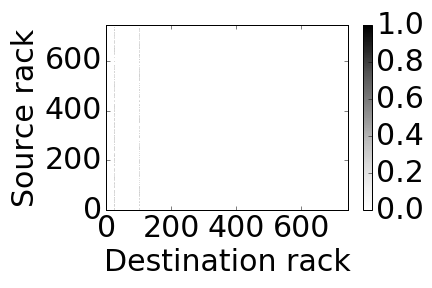
\includegraphics[width=0.3\linewidth]{pictures/ProjecToR1.png}
	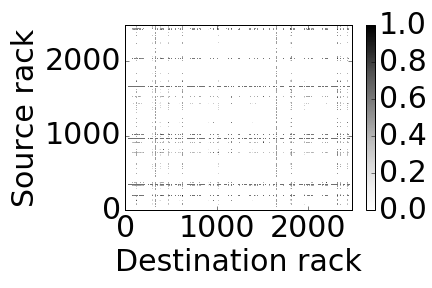
\includegraphics[width=0.3\linewidth]{pictures/ProjecToR2.png}
	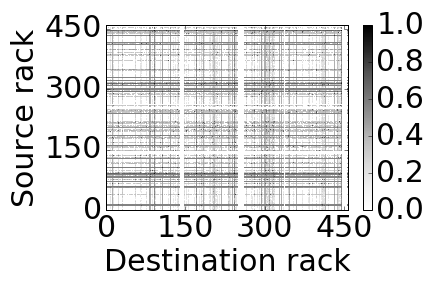
\includegraphics[width=0.3\linewidth]{pictures/ProjecToR3.png}
	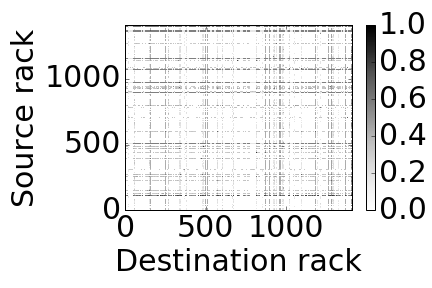
\includegraphics[width=0.3\linewidth]{pictures/ProjecToR4.png}
	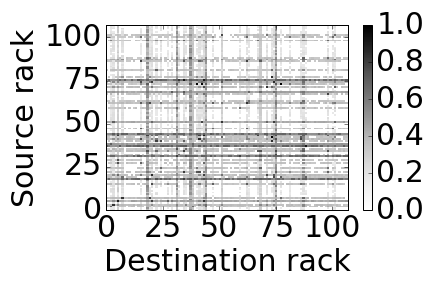
\includegraphics[width=0.3\linewidth]{pictures/ProjecToR5.png}
	\caption{Microsoft adatközpont adatok klaszterenként}
	\label{microsoft-clasters}
\end{figure}

Amint a \ref{microsoft-clasters} ábrán látható, a kommunikáció főleg megadott szerverek között történik.
Korábban már említve volt, az adatközpontok jelenleg a legrosszabb esetre vannak tervezve, hogy bármelyik két szerver tudjon kommunikálni.
Az ábrán látszik, hogy melyik szerverek között nem szükséges feltétlen direkt kapcsolatot kiépíteni, hanem elég egy már meglévő közvetett útvonalat használni, ahol kicsi a torlódás.
Az ilyen hálózat megtervezéséhez először szükségünk van arra, hogy tudjuk milyen tervezési stratégiák vannak és, hogy az adatközpontok milyen topológiával rendelkeznek jelenleg.

\subsection{Hálózat tervezési stratégiák}

A technika fejlődésével elérhetővé váltak eszközök arra, hogy egy adott hálózatot újrakonfiguráljunk, attól függően milyen terhelés éri.
Egy hálózat korábbi kommunikációs mintái tudnak adni egy jó közelítést arra, hogyan történik a kommunikáció a szerverek között.
Az előző példában láthattuk, hogy a Microsoft adatközpontban milyen a forgalomeloszlást rögzítettek, 
és ez alapján lehet majd újratervezni a hálózatot, figyelve a terheléseloszlásra.
Lehetőség szerint, periodikus újrakonfigurálással akár még nagyobb hatékonyságot is elérhetünk az adatközpontokban.

Két fő optimalizációs megközelítést fogunk megnézni a munka során, ezek a rövid úthossz és a minimális torlódás.
Rövid úthossz alatt azt értjük, hogy minél kevesebb pontok kelljen áthaladnia az adatnak mielőtt az eljut a céljába, \ref{network_strategies} ábrán az (a) eset.
A minimális torlódás alatt pedig azt értjük, ha több adatfolyam halad át egy élen, akkor az élek egyenletesen legyenek kihasználva, ezzel csökkentve a várakozási időt, \ref{network_strategies} ábra (b) pontja.
A cikk célja, egy olyan módszer bemutatása, ahol mindkét esetet figyelembe veszik és az alapján adnak egy olyan algoritmust, ami közel optimális mint úthosszra, mint torlódásra nézve, ez a \ref{network_strategies} ábra (c) esete.


\begin{figure}[h]
	\centering
	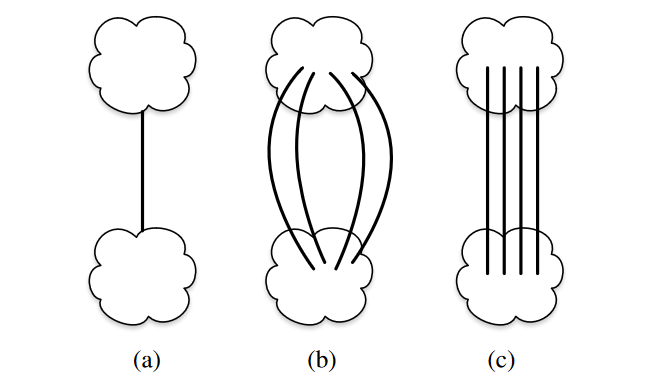
\includegraphics[width=8cm]{pictures/optimalshemes.png}
	\caption{Hálózat tervezési stratégiák, (a) rövid utakra való optimalizálás, (b) minimális torlódásra való optimalizálás, (c) mindkét esetre való optimalizálás}
	\label{network_strategies}
\end{figure}

\subsection{Adatközpontok hálózati felépítése}

\begin{figure}[h]
	\centering
	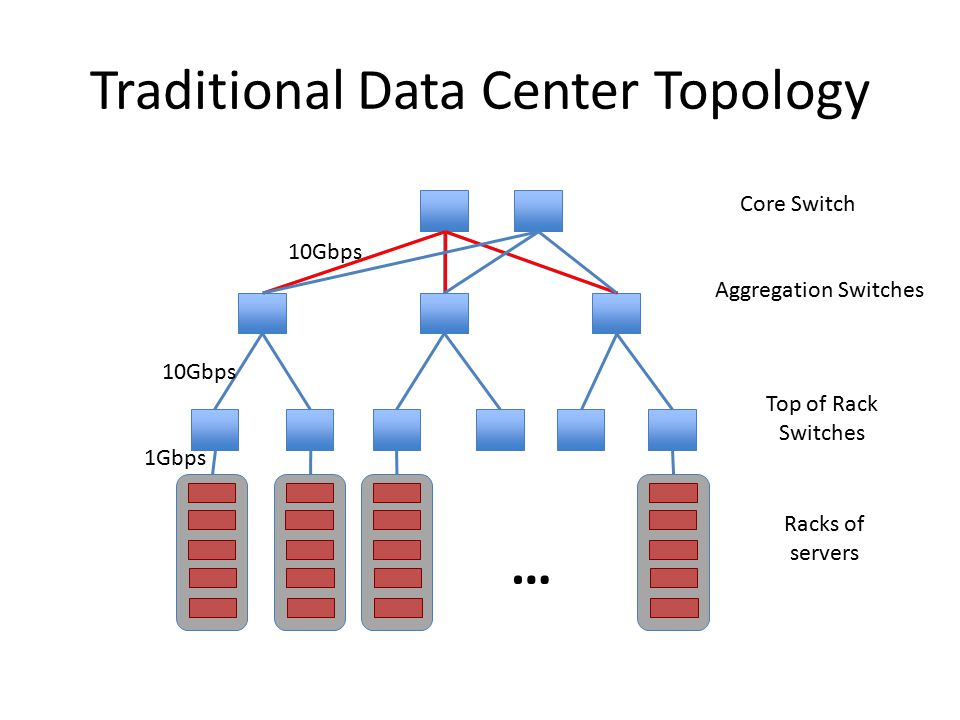
\includegraphics[width=0.7\linewidth]{pictures/Traditional+Data+Center+Topology.jpg}
	\caption{Adatközpont hálózati topológiája}
	\label{datacenter_topology}
\end{figure}

Mielőtt még bármi nemű átalakítást végeznénk az adatközpont hálózatán, először még meg kell nézni azt, hogy hogyan is épül fel az.
Az \ref{datacenter_topology} ábrán látható a felépítés, ahol három szintre tudjuk felosztani a hálózat architektúráját \cite{noauthor_you_nodate} \cite{noauthor_cisco_nodate}.
Legfelső szinten van a Core réteg, ami adja a gerincét a hálózatnak, ezen a ponton érkeznek és távoznak a csomagok az adatközpontból.
A Core réteg további szerepe még, hogy adatot szolgáltasson az alatta lévő Aggregációs rétegnek.
Ez a réteg nagyobb csoportokra osztja az adatközpontot, ezzel minimalizálva a routing táblák számát.
Az aggregációs réteg további szolgáltatásokat is tud nyújtani, az alatta lévő rétegnek, mint például fűzfal, load balancing és biztonságos csatlakozás.
A harmadik réteg pedig a Access réteg, ami Top of Rack switchek formájában nyilvánul meg.
Ezen a ponton kapcsolódnak a szerverek fizikailag a hálózathoz.
A Core rétegtől a ToR switchekig általában optikai kábellel van kiépítve a hálózat. 
ToR switchtől már hagyományos módszerekkel csatlakoznak a szerverek.
Egy rackben nagyon sok szerver van elhelyezve, ezért azok általában egy köztes, úgy nevezett In-Rack switchre kapcsolódnak, amik végül csatlakoznak a hozzájuk legközelebbi ToR switchhez.



\subsection{Újrakonfigurálás megvalósítása}

Az átlag hálózatok statikusan vannak konfigurálva, ezért nem sok lehetőség van arra annak megváltoztatására, ide tartoznak a hagyományos Ethernet switchek.
Egy kevésbé statikus megoldás az optikai swtich, ami képes megvalósítani az újrakonfigurálást, és ezt relatív gyorsan is csinálja.
Az optikai switchektől egy még gyorsabb megoldás a Microsoft Research ProjecToR. 
A \ref{projector-fig} ábrán látható eszköz szem számára láthatatlan lézer nyalábbal küld és fogad adatokat.
Az adatközpont belső kommunikációjának a gyorsítására szolgál, ezért a ToR switchek vannak lecserélve, ilyen ProjecToR eszközökre.
A rack tetejéről az eszköz a lézert mikrotükrökre irányítja, aminek a pontos beállíthatósága révén pontosan a megfelelő irányba tudja tükrözi tovább a nyalábot.
Ennek az folyamatnak köszönhetően jelentősen gyorsabb átkonfigurálási időt érhetünk el mint az optikai switch.
Váltásidő itt $12\mu s$ ami kétszázötvenezerszer gyorsabb mint az optikai switch.

\begin{figure}[h]
	\centering
	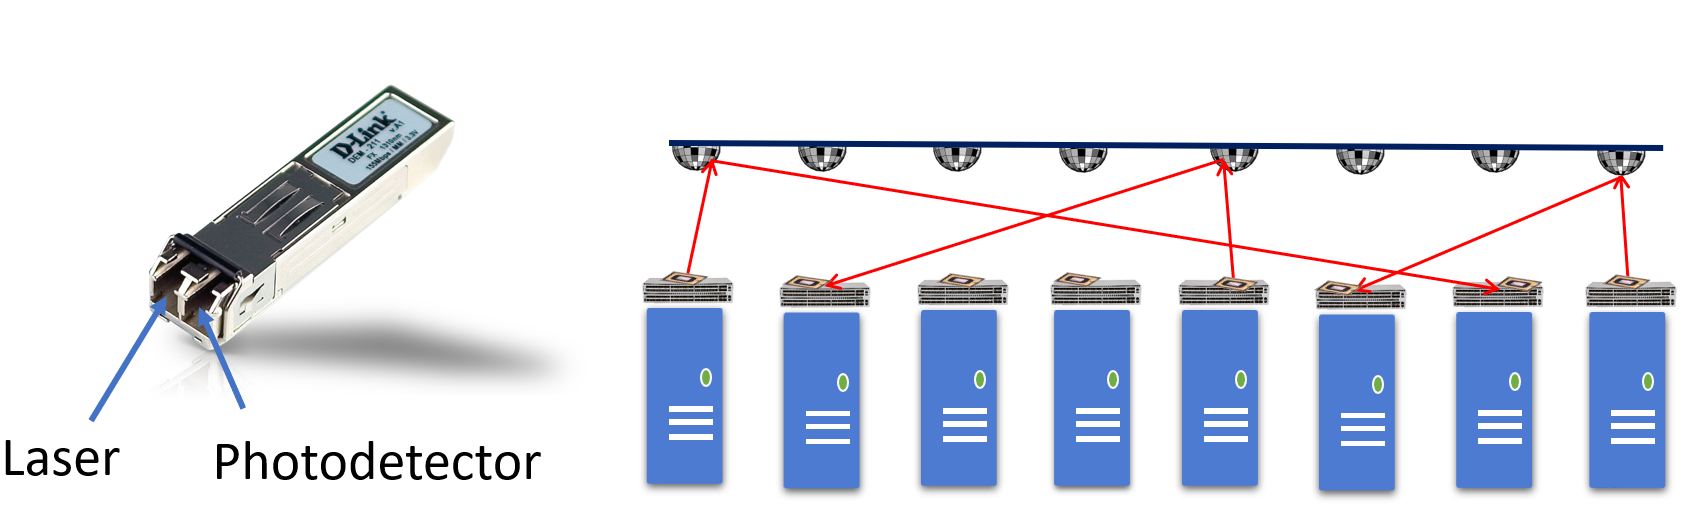
\includegraphics[width=0.9\linewidth]{pictures/laserswitch.png}
	\caption{ProjecToR}
	\label{projector-fig}
\end{figure}

\section{Diplomamunka célja}

A diplomamunka célja a cikkben \cite{avin_demand-aware_nodate} bemutatott algoritmus implementálása.
Ezt egy olyan környezetben megvalósítani, ahol empirikus módszerekkel tesztelhető az algoritmus hatékonysága.
Ez mellet a keretrendszer könnyen kiegészíthető legyen tesztelés szempontjából.
Továbbá lehetőséget biztosítson arra, hogy új algoritmust lehessen bevezetni és azt hasonlóan megvizsgálni, mint az eredetit.
A megvalósítás így több független modulból áll, amik egyként fognak működni.
Az így kapott összes eredményét összehasonlítjuk a cikkben megadott elméleti korlátokkal.

\section{Diplomamunka felépítése}

A diplomamunka felépítése több részre van bontva.
\begin{itemize}
	\item Először ismertetésre kerül az eredeti cikkben \cite{avin_demand-aware_nodate} publikált algoritmus és a hozzá tartozó szükséges háttérismeret.
	\item A második részben szó fog esni a három véletlen gráfról, ami adta az alapot a tesztelésre.
	\item Ezt folytatva ki lesz térve négy darab új algoritmusra, ami valamilyen szempontból változtat a fa építési stratégián annak érdekében, hogy jobb eredményt érjünk el.
	\item A fa építési algoritmusok után, megvizsgáljuk azt az esetet, hogy mi történik, ha már a legelső lépésben módosítjuk az algoritmust, ezzel mérlegelve azt mi kerüljön valóban átépítésre a hálózatban.
	\item Végül következik a tesztelés és annak kiértékelése, milyen teljesítményt nyújtanak a különböző algoritmusok a különböző véletlen gráfok esetén. 
\end{itemize}


\section{Diplomamunka eredménye}

A diplomamunka véletlen gráfokkal modellezte a adatközpontokban kialakulható hálózati forgalmat.
Az eredmények azt mutatják, hogy a cikkben meghatározott "optimális" eset egy határozottan magasabb felső korlát, mint amire valójában szükség van.
Az cikkben felvázolt algoritmus némi helyet hagy az megvalósítónak, mivel nem teljesen írja le pár helyzetben mi a helyes lépés.

Ez alapján született kettő algoritmus, az Eredeti és az EgoBalance, ami az egyik ilyen rész miatt más-más értelmezésben próbálta megoldani a felmerülő helyeztet.
A teljesség érdekében egy másik megközelítési módszer is vizsgálva volt, mint fa építési stratégia, ami további három algoritmust eredményezett, ezek rendere a Huffman-, Sorfolyotonos- és Véletlen fák voltak.
Ezek az algoritmusok az úthosszt vették figyelembe és itt jól is teljesítettek, de torlódás szempontjából alul múlták a cikkben szereplőt közel egy kettes szorzóval.
Ebből kifolyólag a cikkben szereplő algoritmus megfelelő a céljára, de nem zárja ki a lehetőséget egy másfajta javítási megközelítésre. 

A második javítási mód előtérbe helyezi azt a szempontot, hogy mérlegeljük a hálózatban szereplő ténylegesen leterhelt pontokat és azokat építjük át csak.
Ezzel elejét vehetjük az olyan esteknek, hol nincs szükség átépítésre.
Ezzel csökkenthetjük a számítás igényét az algoritmusnak és egyúttal még rövidebb utakat is érünk el az új hálózatban.
Ez a javítás nincs kihatással a torlódásra az esetek túlnyomó részében, de vannak elfajult esetek ahol rosszabbat eredményez.



\chapter{Modell}


A diplomamunkában a \cite{avin_demand-aware_nodate} cikkben leírt modell és definíciók lettek használva.

\section{Forgalom igény tudatos hálózat tervezés probléma}

Egy hálózat forgalomigényének nevezzük azt a mátrixot, mi leírja melyik csomópontok állnak kapcsolatban és mekkora valószínűséggel kommunikálnak.
Ez a mátrix legtöbb esetben szimmetrikus, de lehetnek esetek egy oldali kommunikációra is, például egy archiváló szerver, ami nem küld vissza információt a küldőjének.

Forgalom igény tudatos hálózat tervezés problémának nevezzük azt, mikor rendelkezésre áll egy meghatározott számú csomóponttal rendelkező hálózat és egy mátrix ami leírja a kommunikációs mintát.
A mátrix elemei súlyozott valószínűségek, hogy $i$ forrásból mekkora eséllyel lesz adat küldve $j$ célba.
A cél, hogy ezen adatból egy olyan hálózati sémát készítsünk, ami minimális torlódást és rövid utakat eredményezzen és ez mellett még skálázható is legyen nagy hálózatokra.

A \ref{network_types} ábrán látható egy demand mátrix és a két megközelítés, ami alapján vizsgálni az új hálózatot.

\begin{figure}[h]
	\centering
	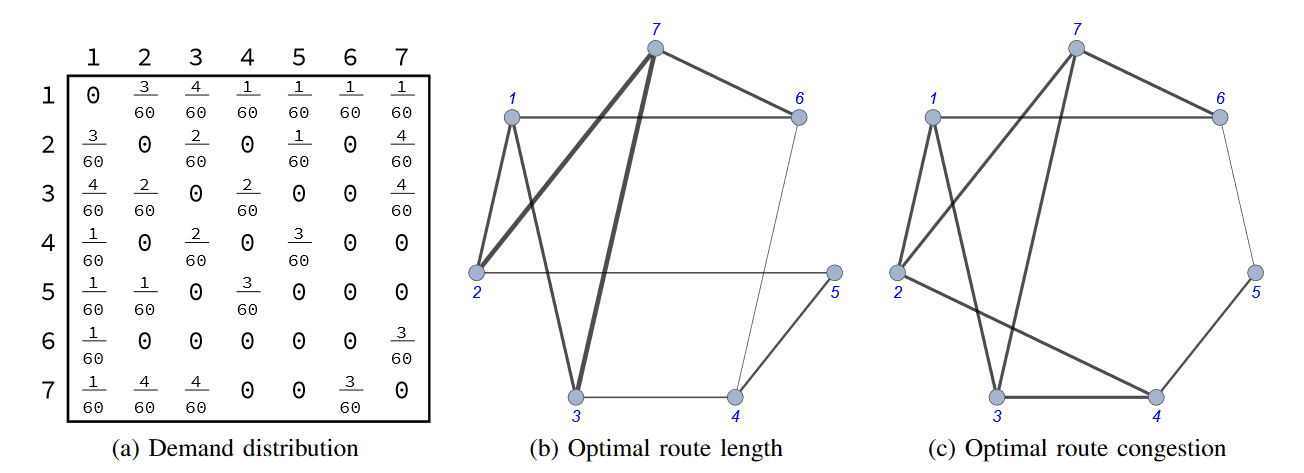
\includegraphics[width=14cm]{pictures/example.png}
	\caption{Forgalom igény tudatos hálózat tervezés probléma, (a) demand mátrix, (b) hálózat optimális úthosszra és (c) hálózat optimális torlódásra}
	\label{network_types}
\end{figure}

\section{Formális definíció}



Adott $N$ darab csúcspont  $V = \{1, ..., N\}$  és egy $M_D$ kommunikációs séma, ami egy $N\times N$ mátrix.
A mátrix $(i, j)$ eleméhez tartozik egy $p(i, j)$ valószínűség, ahol $i$ a forrás, $j$ pedig cél csomópont.
A bemeneti mátrix ábrázolható egy irányított $G_D$ gráfban, ahol az élsúlyok a két pont közötti kommunikációs valószínűséget írják le.
Az algoritmus feltétele, hogy a \(M_D\) mátrix ritka legyen.
Egy $N$ hálózatra a torlódást és az úthosszt az útválasztási sémával fogjuk definiálni.
Egy útválasztási séma az $N$ hálózatra a $\Gamma(N)$, ami $\Gamma_{uv}$ utak halmaza, ahol $(u, v)$ párok különböző utakat jelölnek.
$\Gamma_{uv}$ egy útsorozat, ami összeköti az $u$ pontot $v$ ponttal.

\subsection{Torlódás}

\begin{mydef}
	A torlódást egy \(\Gamma(N)\) útválasztási sémán a \(D\) demand mátrix segítségével írjuk fel: \[C(D, \Gamma(N)) = \max_{e \in \Gamma(N)}  \sum_{e \in \Gamma(uv)} p(u,v) \]
\end{mydef}

Szavakba foglalva, a torlódás megegyezik az útválasztási sémában szereplő legjobban leterhelt úttal.

\subsection{Úthossz}

\begin{mydef}
	Az átlag súlyozott úthosszt egy \(\Gamma(N)\) útválasztási sémán a \(D\) demand mátrix segítségével írjuk fel: \[L(D, \Gamma(N)) = \sum_{(u,v) \in D}  p(u,v)  \cdot d_{\Gamma(N)}(u, v) \] ahol a \(d_{\Gamma(N)}(u, v)\) az útvonal hosszát jelöli.
\end{mydef}

Szavakba foglalva, az átlag súlyozott úthossz, az összes út összege, ahol a csomópontok közötti utak hossza meg van szorozva a valósínűségükkel. 

\subsection{Skálázhatóság}

A hálózatot skálázhatóra kell tervezni, ezért meghatározunk egy \(\Delta\) konstans fokszámot, ami a maximális csatlakozások számát fogja meghatározni egy adott csomóponthoz.
\(N_\Delta\) jelölje az összes \(\Delta\) fokszámú gráfot, és elváruk, hogy \(N \in N_\Delta\).


\subsection{Optimális torlódás}


Az optimális torlódást egy  hálózatra, úgy határozzuk meg, hogy a csak a torlódást vesszük figyelembe számításkor: 
\[C^*(D, \Delta) = \min_{N \in N_\Delta, \Gamma(N)} C(D, \Gamma(N))\]


\subsection{Optimális úthossz}

Az optimális úthosszt egy  hálózatra, úgy határozzuk meg, hogy a csak az úthosszt vesszük figyelembe számításkor:
\[L^*(D, \Delta) = \min_{N \in N_\Delta, \Gamma(N)} L(D, \Gamma(N))\]

\section{cl-DAN hálózat tervezése}

\begin{mydef}
	Adott egy \(D\) demand mátrix, és egy \(\Delta\) maximális fokszám, az \((\alpha, \beta)\)-cl-DAN hálózat tervezési probléma:
	\begin{itemize}
		\item Hogy tervezzünk egy olyan \(N \in N_\Delta\) hálózatot, és egy hozzá tartozó \(\Gamma(N)\) útválasztási sémát, ami közel optimális torlódásra és úthosszra is?
	\end{itemize}
	
	Az algoritmus egy felső korlátot tud adni arra, hogy mennyivel fog eltérni a megoldás az optimálistól, ami a következő:
	\begin{itemize}
		\item Torlódásra: \(C(D, \Gamma(N)) \le \alpha \cdot C^*(D, \Delta) + \alpha'\)
		\item Úthosszra: \(L(D, \Gamma(N)) \le \beta \cdot L^*(D, \Delta) + \beta'\)
	\end{itemize}
	Az alfa vessző és béta vesszők olyan tényezők aki amik függetlenek a problémától.
\end{mydef}

\section{EgoTree}

Az Egófa egy torlódásra és úthosszra optimalizált fa hálózat egy csomópontra nézve.
Az Egófát a következő módon definiáljuk:
	
\begin{mydef}
	Az \(EgoTree(s, \bar{p}, \Delta) \) egy fa hálózat, ahol
	\begin{itemize}
		\item \(s\) a forrás csomópont
		\item \(\bar{p}\) a szomszédainak eloszlásai
		\item \(\Delta\) fokszám
	\end{itemize}
\end{mydef}

Ez közel optimális megoldást ad torlódásra és úthosszra.


\begin{mytetel}
	Adott egy  \(\bar{p}\) frekvencia eloszlás az \(s\) forrás ponthoz, és adott egy \(\Delta\) fokszám, ekkor az \(EgoTree(s, \bar{p}, \Delta)\) egy \((\alpha, \beta)\)-cl-DAN a következő paraméterekkel:
	\begin{itemize}
		\item \(\alpha = \frac{4}{3}\)
		\item \(\beta = log^2(\Delta + 1)\)
	\end{itemize}
\end{mytetel}

\subsection{EgoTree algoritmus}

Az Egófa megépítésére a következő algoritmust használjuk:

\begin{enumerate}
	\item \(s\) a gyökér elem, \(\Delta\) fokszámmal, kezdetben üres fa.
	\item Rendezzük csökkenő sorrendbe a \(\bar{p} = \{p1, p2, ..., p_k\}\) valószínűségeket 
	\item Kezdjük a gyökér elemre csatolni a csomópontokat, legfeljebb \(\Delta\) kapcsolat állhat fent a gyökérrel.
	\item Mikor elértük a \(\Delta\) kapcsolatot a gyökér elemnél, a következő csomópontokat mindig a legkisebb összesített súlyú levélre kapcsolok rá, itt már legfeljebb két levele lehet minden fának.
\end{enumerate}

\begin{figure}[H]
	\begin{center}
		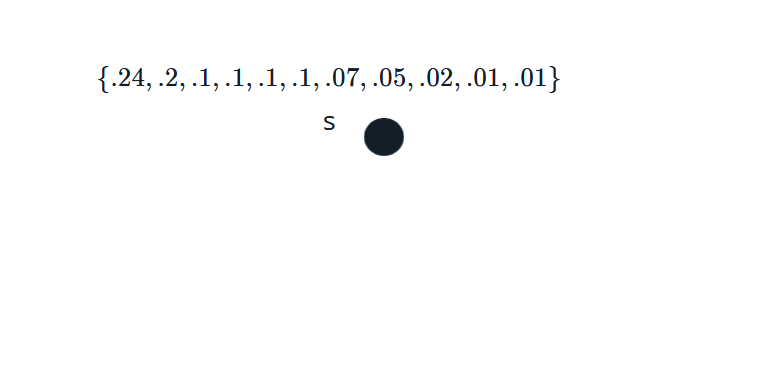
\includegraphics[width=0.49\linewidth]{pictures/egofa1.png}
		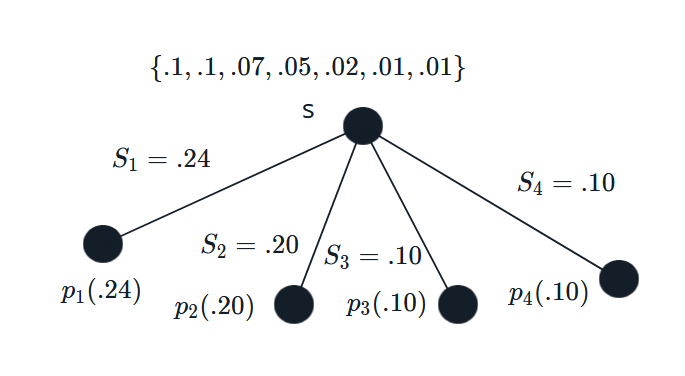
\includegraphics[width=0.49\linewidth]{pictures/egofa2.png}
		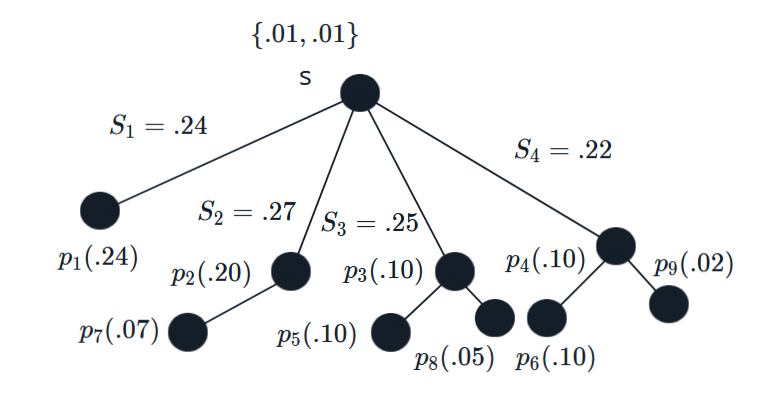
\includegraphics[width=0.49\linewidth]{pictures/egofa3.png}
		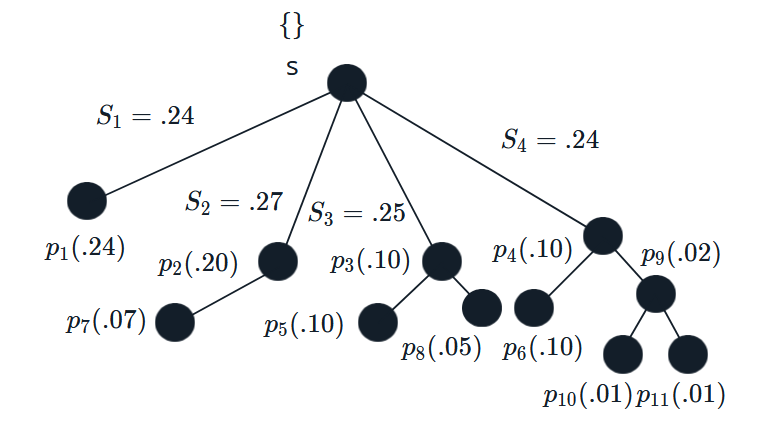
\includegraphics[width=0.49\linewidth]{pictures/egofa4.png}
		\caption{Egófa algoritmus lépéseinek vizualizációja a következő valószínűségekre: 
			\( \{.24, .2, .1, .1, .1, .1, .07, .05, .02, .01, .01\}\)}
		\label{egotree-algorithm}
	\end{center}
\end{figure}


\subsection{Algoritmus elemzése}

A kapott eredményben látható, hogy a maximális torlódás a legnagyobb súlyú élen van.
Minimalizálni ezt, lényegében egy időzítés probléma, hogy osszuk ki a munkákat \(\Delta\) processzornak, hogy a munka a leghamarabb kész legyen.
Erre az optimális algoritmus NP-nehéz, de van közelítő módszer.

\subsection{Longest Processing Time (LPT)}

A Longest Processing Time algoritmus a következő:

\begin{itemize}
	\item Először rendezzük sorba a feladatokat hossz szerint csökkenő sorrendbe.
	\item Ha van szabad processzor, akkor rendeljük hozzá a leghosszabb munkát
	\item Ha nincs szabad processzor, akkor ahhoz a processzorhoz rendeljük hozzá a következő munkát, ahol a legkevesebb ideig tart a munka.
\end{itemize}

\begin{mytetel}
	Legyen \(\omega_L\) a maximum idő, mielőtt egy processzor befejezi az összes munkát a mohó LPT algoritmus szerint, és \(\omega_0\) az optimális, ekkor \[\frac{\omega_L}{\omega_0} \le \frac{4}{3} - \frac{1}{3\Delta}\]
\end{mytetel}

Ez az algoritmus polinom időben lefut.

\begin{mylemma}
	Az \(EgoTree(s, \bar{p}, \Delta)\) ad egy \(\frac{4}{3}\) szorzóval nagyobb közelítést a minimális torlódásra az optimális \(\Delta\) fokú fához képest, ami kiszolgál \(\bar{p}\) frekvencia eloszlást egy adott \(s\) forrás csomópontra.
\end{mylemma}

\begin{mylemma}
	Az \(EgoTree(s, \bar{p}, \Delta)\) ad egy \(log^2(\Delta + 1)\) szorzóval nagyobb közelítést a minimális úthosszra az optimális \(\Delta\) fokú fához képest, ami kiszolgál \(\bar{p}\) frekvencia eloszlást egy adott \(s\) forrás csomópontra.
\end{mylemma}

\section{cl-DAN algoritmus}

\begin{mytetel}
	Legyen \(D\) egy szimmetrikus kommunikáció kéréseloszlás , ahol az átlag csúcs fokszáma \(\rho\), (azaz az élek száma \(\rho \cdot \frac{n}{2}\). Ekkor a maximum fokszám \(\Delta = 12\rho\), ehhez lehetséges generálni egy \((\alpha, \beta)\)-cl-DAN hálózatot, ahol:
	\begin{itemize}
		\item \(\alpha = 1 + (\frac{8}{9})\Delta\)
		\item \(\beta = 1 + 4log^2(\Delta + 1)\)
	\end{itemize}
\end{mytetel}
Konstans \(\rho\) esetén ez konstans közelítést ad a minimális torlódásra és az optimális úthosszra

\begin{enumerate}
	\item Felosszuk a hálózat csúcsait két halmazra, \(H\) - magas és \(L\) - alacsony fokszámúakra fele-fele arányban
	\begin{itemize}
		\item Az alacsony fokszámú csúcsok fokszáma legfeljebb \(2\rho\)
	\end{itemize}
	\item Megkeressük az összes olyan \((u, v)\) élt, ahol \(u\) és \(v\) is a magas fokszámú halmazba tartozik
	\item Az ilyen éleket a gráfban kiegészítjük egy segítő csomóponttal, \(l \in L\), az eredeti csomópontok között megszüntetjük az élt, és felveszünk két új élt \((u, l)\) és \((v, l)\)
	\begin{itemize}
		\item Minden segítő \(l\) csúcs választásakor egy még nem felhasználtat válasszunk az \(L\) halmazból
	\end{itemize}
	\item Meghatározunk egy mátrixot, ami első lépésben az eredeti
	\begin{itemize}
		\item Ahol segítő csomópontot vettünk fel, ott az útvonal hosszúhoz hozzá kell még adni az \(l\)-el való áthaladást is, és törölni kell az eredeti pontok közti élt
		\item Ezután elkészítjük a magas halmaz csúcsaira a \(T_u\) fát, ahol a valószínűségeket a mátrixból kiolvassuk, \(\Delta = 12\rho\) fokszámmal, ez közel optimális megoldást ad mindkét fel
	\end{itemize}
	\item Mivel \(u\) és \(v\) pontok közt egy \(l\) segítő csomópont van használva ezért \(T_u\) és \(T_v\) módosításra szorul. Alakítsuk át először \(T_u\)-t \(T'_u\)-ra
	\begin{itemize}
		\item Ha \(l \notin T_u\), \((p(u, l) = 0)\), akkor \(l\) átveszi \(v\) helyét \(T'_u\)-ban
		\item Ha \(l \in T_u\), \((p(u, l) > 0)\), akkor két lehetőségünk van:
		\begin{itemize}
			\item Ha \((p(u, l) > (p(u, v))\), akkor töröljük \(v\)-t a fából
			\item Ha \((p(u, l) \le (p(u, v))\), akkor \(l\) átveszi \(v\) helyét \(T'_u\)-ban
		\end{itemize}
		\item \(T'_v\) hasonlóan számítjuk ki, ezzel garantálva, hogy \(T'_u\) és \(T'_v\) közötti kommunikáció az \(l\) csomóponton keresztül fog áthaladni
	\end{itemize}
	\item Konstruáljuk meg az új N hálózatot, vegyük az előbb készített egófákat és vegyük az uniójukat, azaz húzzuk be az összes olyan élet amik szerepeltek a fákban
	\begin{itemize}
		\item     De mivel nem csak magas fokú csomópontok közt történhetett adatforgalom, ezért még vegyük hozzá az N hálózathoz azokat az éleket is, ahol mindkét csomópont alacsony fokszámú volt
	\end{itemize}
\end{enumerate}

\chapter{Kiterjesztett modell}

\section{Véletlen gráfok}

A hálózat tesztelésnek céljából több különböző típusú véletlen gráfon lett tesztelve az algoritmus hatékonysága.
A következő alfejezetekben ezek lesznek bemutatva.

\subsection{Barabási-Albert modell}

A Barabási-Albert modell \cite{RevModPhys.74.47} a komplex hálózatok egy modellje. 
A \(G(n, m)\) gráf felépítése az úgy nevezett "preferential attachment" mechanizmust használja, ami kimondja, hogy az újonnan becsatlakozó csomópontnak \(m\) már a hálózatban szereplő csomópontra kell kapcsolódnia. A \ref{barabasi} ábrán látható a gráf eredménye, attól függően, hogyan választjuk meg az \(m\) értéket.

\begin{figure}[H]
	\begin{center}
		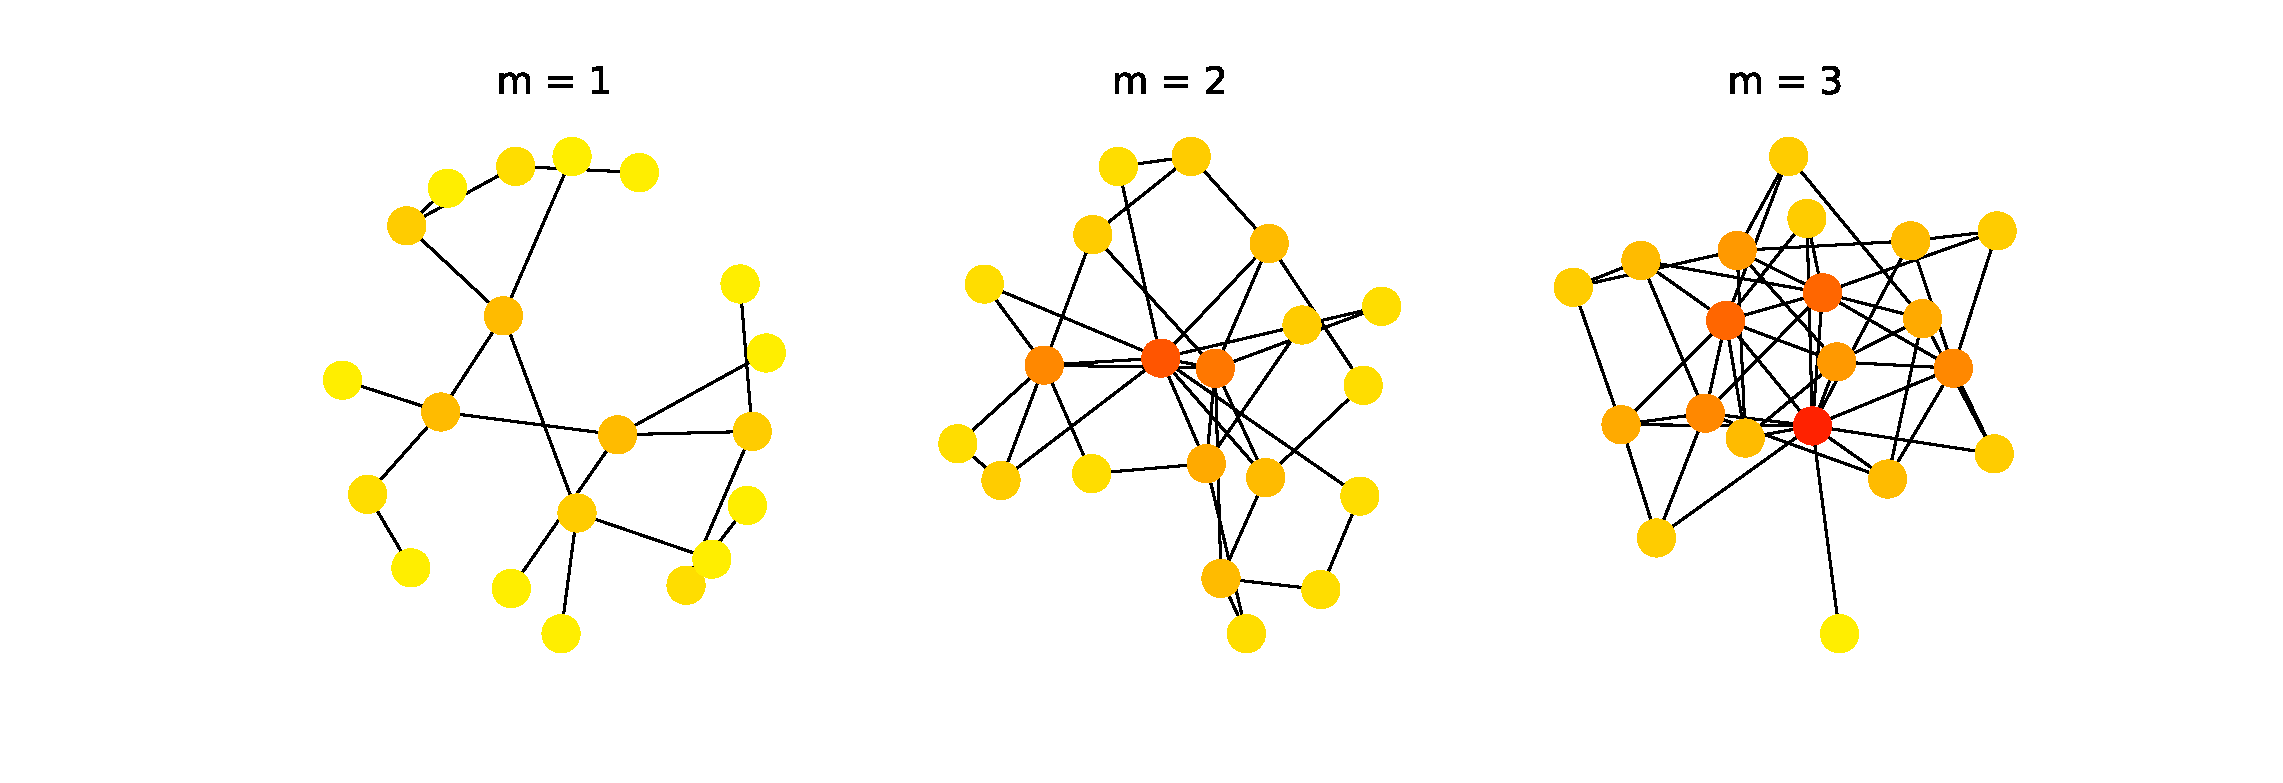
\includegraphics[width=0.9\linewidth]{pictures/Barabasi_albert_graph.eps}
		\caption{Barabási-Albert gráf \cite{wikipedia_barabasi}}
		\label{barabasi}
	\end{center}
\end{figure}

\pagebreak

\subsection{Erdős-Rényi modell}

Az Erdős-Rényi modell \cite{erdos59a} a véletlen gráfok előállítására szolgáló modell.
A modellnek két változata van, amik szorosan összefüggenek.
\begin{itemize}
	\item A \(G(n, M)\) modellben egyenletes eloszlás szerint választunk egyet az összes lehetséges \(n\) csúcsú gráf közül, ahol az élek száma \(M\).
	\item A \(G(n, p)\) modellben az \(n\) csúcsú gráf éleit \(p\) valószínűséggel húzunk be bármely két csúcs között, egymástól függetlenül.
\end{itemize}

A \ref{erdos} ábrán látható egy lehetséges véletlen gráf \(p=0.01\) valószínűséggel.

\begin{figure}[H]
	\begin{center}
		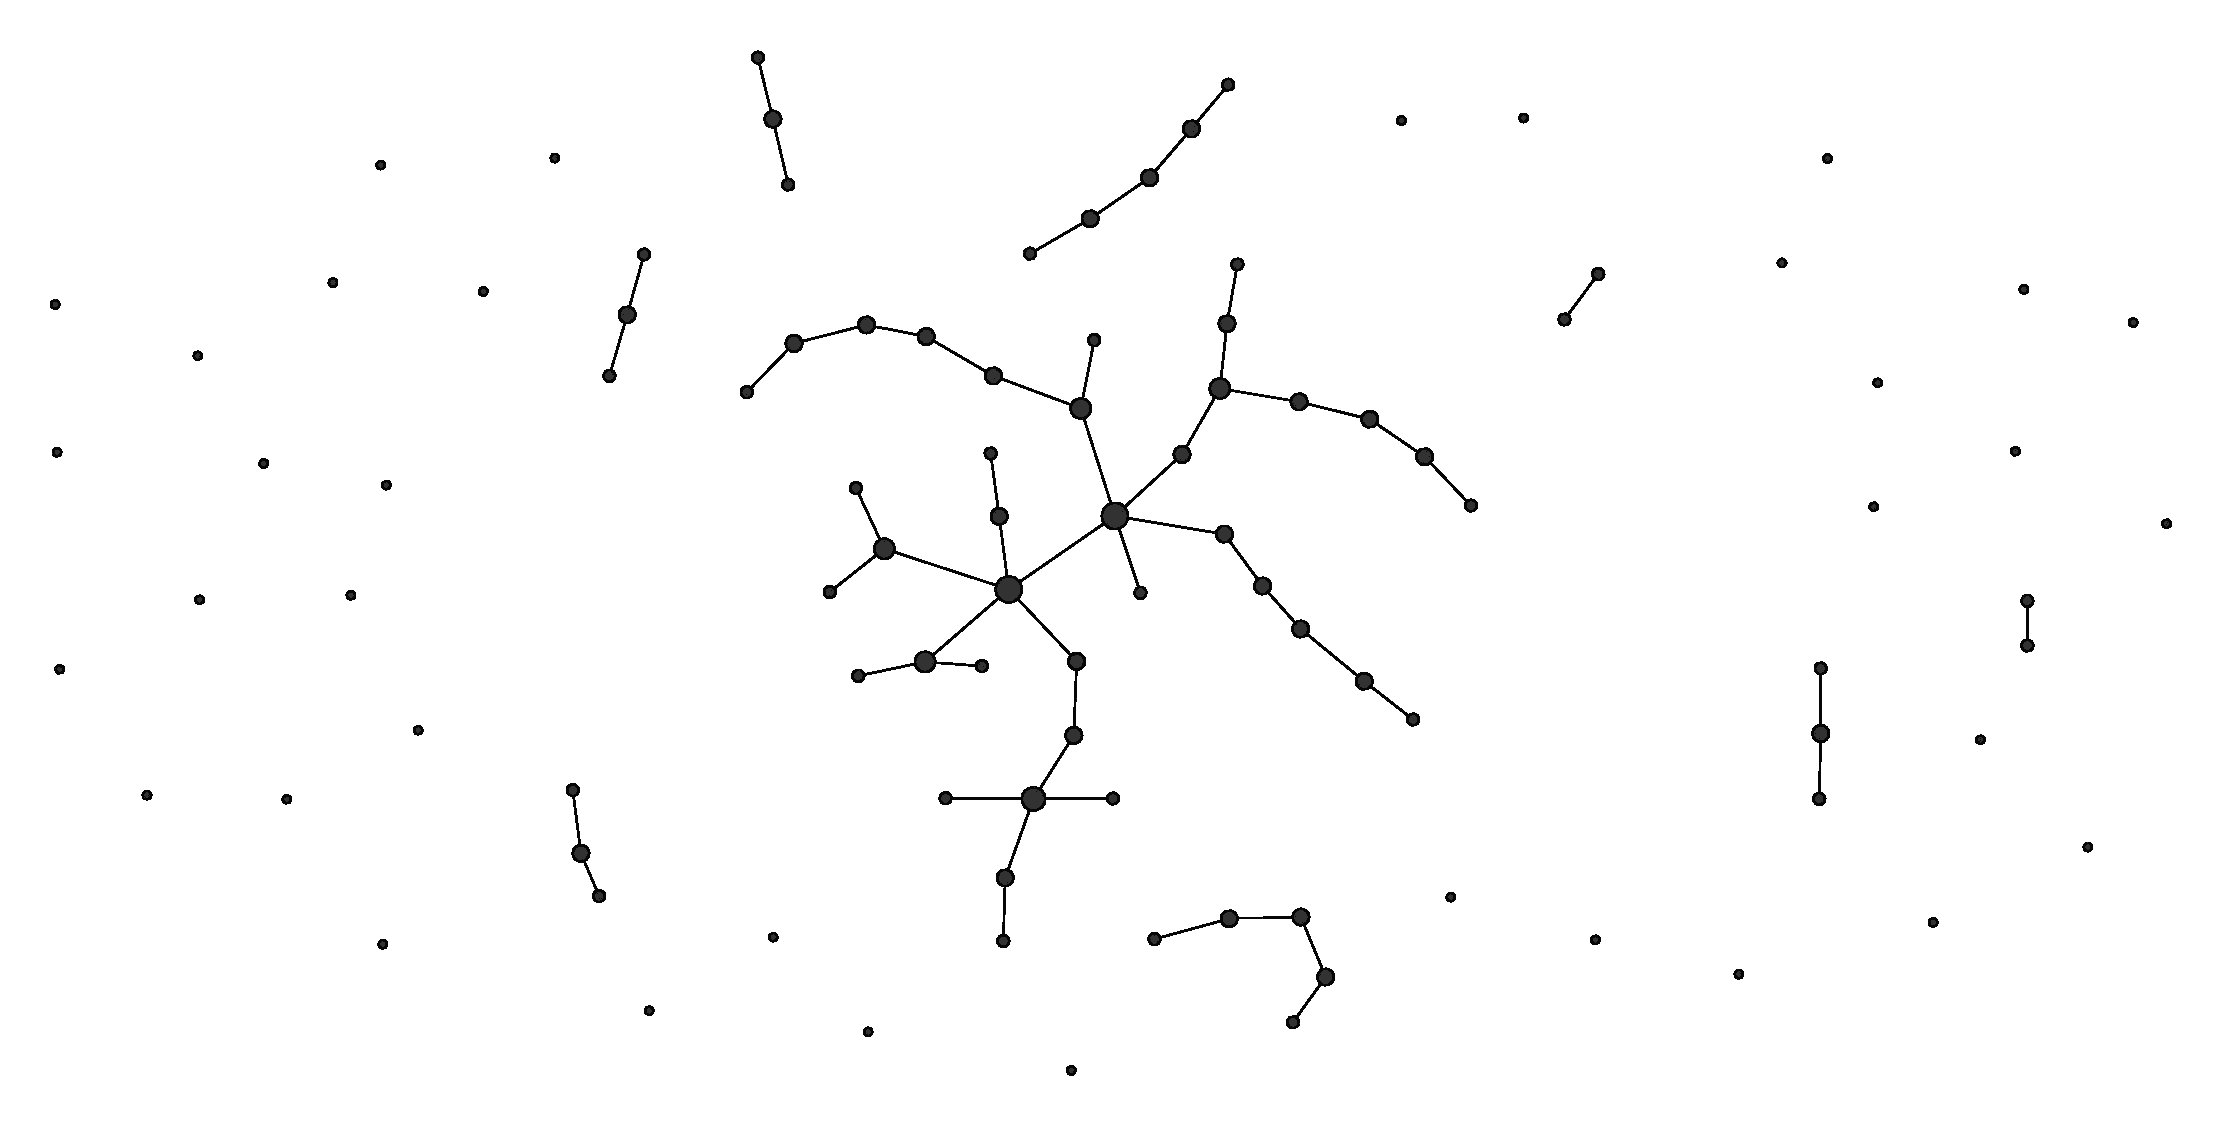
\includegraphics[width=0.9\linewidth]{pictures/Erdos_generated_network-p001.jpg}
		\caption{Erdős-Rényi gráf \(p=0.01\) valószínűséggel \cite{wikipedia_erdos}}
		\label{erdos}
	\end{center}
\end{figure}

A munka során a második megközelítést volt használva a véletlen gráfok generálására.

\subsection{Csillaggráf}

A csillaggráf vagy röviden csillag, egy olyan gráf, ahol \(n\) csúcs esetén, van egy központi csúcs a gráfban amivel a maradék \(n-1\) csúcs kapcsolatban áll.
Bármely két csúcs, amelyek közül egyik sem a csillag közepe, nem áll kapcsolatban.
A \ref{star} ábrán látható egy példa a nyolc csúcs gráfra ahol egy csillag van.
A munka során használt véletlen csillaggráfokban a csillagok számát lehet megadni.

\begin{figure}[H]
	\begin{center}
		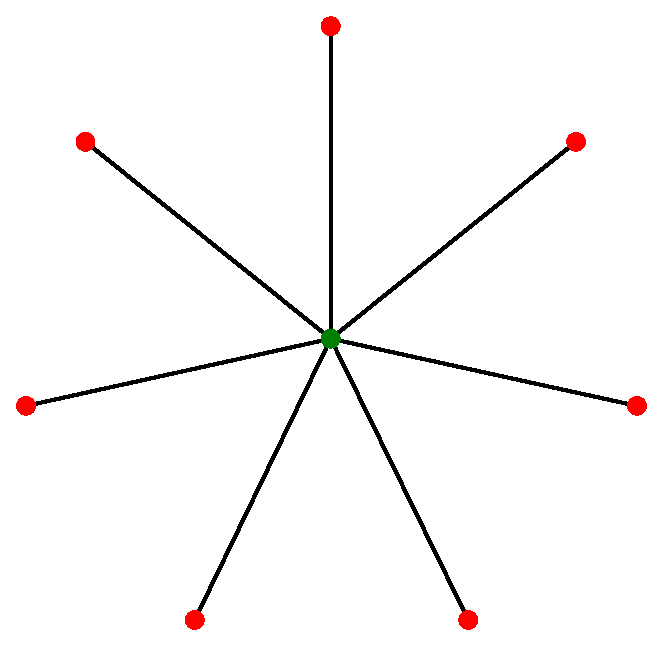
\includegraphics[width=0.4\linewidth]{pictures/Star_network_7.eps}
		\caption{Csillaggráf hét fokszámmal, \(S_7\) \cite{wikipedia_csillag}}
		\label{star}
	\end{center}
\end{figure}

\section{Fa építési stratégiák}

A cikkben \cite{avin_demand-aware_nodate} már szereplő Egófa algoritmusából kiindulva több különböző fa építési stratégia is meg lett valósítva.
A különböző fa építési stratégiák más-más szempontból közelítik meg a problémát.

\subsection{EgoBalance}

Az EgoBalance algoritmus majdnem teljes mértékben megegyezik az eredetivel.
A cikk szerzői a cl-Dan algoritmus vázlatos összefoglalásában használtak egy csere lépést.
A csere lépés lényege, hogy mikor megépítettük a fát egy magas csúcsra, akkor a fában minden szomszédja megjelenik.
A szomszédok között megtalálhatók a magas-magas fokszámú kapcsolatok, amiket ki kell cserélni a segítő csúcsokra.
Három esetet különböztetünk meg itt, attól függően hol helyezkedik el a segítő csúcs a fában.
Első eset, mikor a segítő csúcs nem szerepel a fában, ilyenkor a magas csúcsot ki kell cserélni a segítőre. Ebben az esetben nem kell semmi kiegészítő lépést csinálni, mivel a gyerekeket átveszi a segítő.
A következő két eset, mikor a segítő is része a fának. 
Attól függően mennyire közel vannak az érintett csúcsok a fa gyökeréhez más-más gyerek csúcsokat kell újra elhelyezni.
Mikor a segítő csúcs közelebb van a gyökérhez, akkor töröljük a magas pontot a fából, ha voltak gyerekei a törölt pontnak, akkor azoknak új szülő csúcsot kell találni.
Ellenkező esetben, mikor magas pont helyezkedik el közelebb a forráshoz, akkor a segítő csúcs átveszi a helyét és gyerekeit, majd a segítő leveleinek kell új szülő csúcsot találni. 
Ezt úgy oldja meg az eredeti algoritmus, hogy a nehezebb levél csúcs lesz az új szülő és a könnyebb csomópontnak ő lesz a szülője.

\pagebreak

Egy lehetséges eset ilyenkor, hogy az új szülő csúcsnak már ki van töltve mindkét levele, ekkor a szülő könnyebb levele fog egyel lejjebb szintre kerülni.
Ezt a folyamatot addig ismételjük, még minden levél nem kerül egy megfelelő helyre.

Az Egobalance algoritmus a függő pontok újra elhelyezését az Egófára bízza, azaz újra elosztásra kerülnek.
Ezzel elméletben mindig arra törekszik az algoritmus, hogy optimális legyen torlódásra nézve az új fa.
Lényegi különbség úthossznál jelentkezik az eredetivel szemben.

\subsubsection{EgoBalance algoritmus}
\begin{enumerate}
	\item Végezzük el a csere lépésig a cl-Dan algoritmust
	\item Mikor csere lépés történik a szülő nélküli csúcsokat kapcsoljuk vissza a fába az Egófa algoritmussal
\end{enumerate}

\subsection{Huffman fa}

A eddigi két algoritmus az Egófát \cite{avin_demand-aware_nodate} használta, ami optimális torlódásra nézve, de mivel a hálózat nem csak torlódás szempontjából van vizsgálva, ezért meg kell vizsgálni a másik aspektust is, az optimális úthosszt.
A Huffman kódolásnál \cite{huf52} használt fa tulajdonsága, hogy átlagosan rövidek legyenek az utak attól függően milyen gyakori egy elem.
A cl-Dan probléma is ezt a tényezőt használja, ezért kitűnően lehet használni ezt a fát a hálózat alapjának.
Egyetlen probléma a Huffman fával az, hogy a belső csomópontok nem tartalmaznak számunkra hasznos információt.
Ezért szükséges egy kiegészítő lépés, ami segítségével belső pontok is ki lesznek töltve, azaz esetünkben csomópontokat fognak reprezentálni, mint a levelek.

Az algoritmus első része teljesen megegyezik a Huffman kódolással.
Rendezzük sorba növekedően a valószínűségeket, és kettesével vonjuk össze őket, még nem kapunk egy teljes fát.
Mint az Egófáknál, úgy a Huffman fánál is a legfelső szinten \(n\) darab csúcsot tudunk a forrás pontra kapcsolni.
Az összes többi alacsonyabb pont pedig marad bináris.

A belső csúcsok kitöltésére a gyökér ágain a következő algoritmust végezzük el:
\begin{enumerate}
	\item Gyűjtsük össze a levelet az ágon, a levelek tartalmazzák a számunkra hasznos pontokat 
	\item Az ág gyökerétől indulva sorfolytonosan helyezzük el a leveleket, ahol a valószínűségek csökkenő sorrendben vannak rendezve
\end{enumerate}

Felmerülhet a kérdés, hogy miért nem a legnehezebb levél jön fel mindig?
Ez azért van, mert a Huffman kódolásnál megtörténik az eset, hogy két csomópont összesített értéke megegyezik egy harmadikkal.
Ez egy olyan fát eredményez, ahol az egyik oldalon egy nehéz csúcs, a másik oldalon pedig két könnyű csúcs szerepel.
A naiv megoldás azt eredményezi, hogy az a nehéz pont lesz a belső csúcs és az ág ahonnan jött megüresedik.
A könnyebb fa levelei nem fognak ágat változtatni, annak ellenére, hogy megüresedett az ág feljebb, ezért hosszú egyenes utak jöhetnek létre.
Ennek kiküszöbölésére van a sorfolytonos algoritmus, ahol garantálni lehet, hogy fa egyik belső pontja sem marad kitöltetlen.

\subsubsection{Huffman fa algoritmus}
\begin{itemize}
	\item Végezzük el a fa építés lépésig a cl-Dan algoritmust, demand mátrix itt már a megváltozott állapotban van, nincs két magas csomópont között direkt kapcsolat
	\item Építsük meg a fákat a következő módon:
	\begin{enumerate}
		\item Vegyük a gyökérhez kapcsolódó csúcsok valószínűségét egy vektorba
		\item Rendezzük a vektort növekvő sorrendbe
		\item Vonjuk össze a vektor legelső két elemét, majd helyezzük vissza a vektorba és rendezzük újra a növekvő sorrendbe
		\item Ezt addig csináljuk elemek száma nem éri el a maximális fokszámot, $\Delta$-át
	\end{enumerate}
	\item Itt megépítettük a Huffman fát, ahol még nincsenek kitöltve a belső csomópontok
	\item A köztes csomópontok kitöltése a következő módon történik:
	\begin{enumerate}
		\item A gyökérre kapcsolódó ágakon gyűjtsük össze az összes levelet
		\item Rendezzük sorba a leveleket nehézség szerint csökkenő sorrendbe
		\item Építsünk teljes fát az ágon 
	\end{enumerate} 
\end{itemize}

\begin{figure}[H]
	\begin{center}
		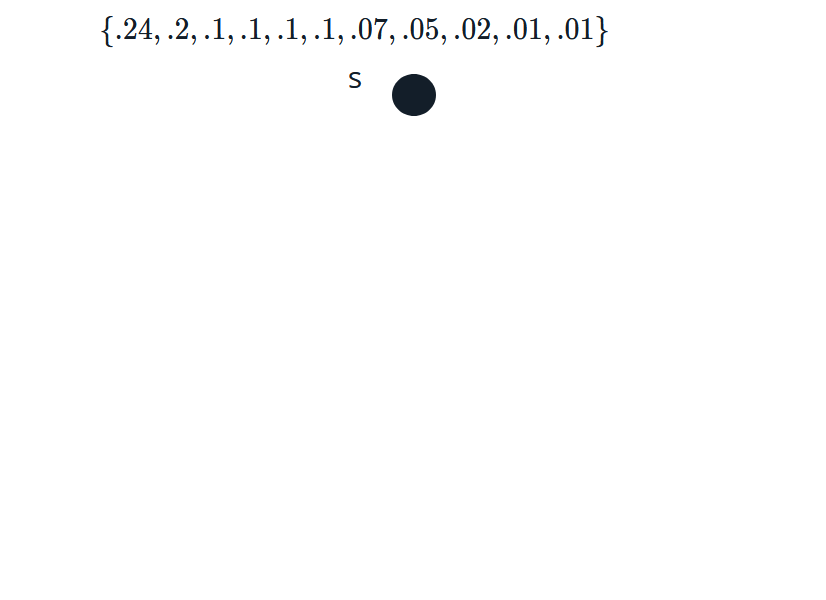
\includegraphics[width=0.49\linewidth]{pictures/huffman1.png}
		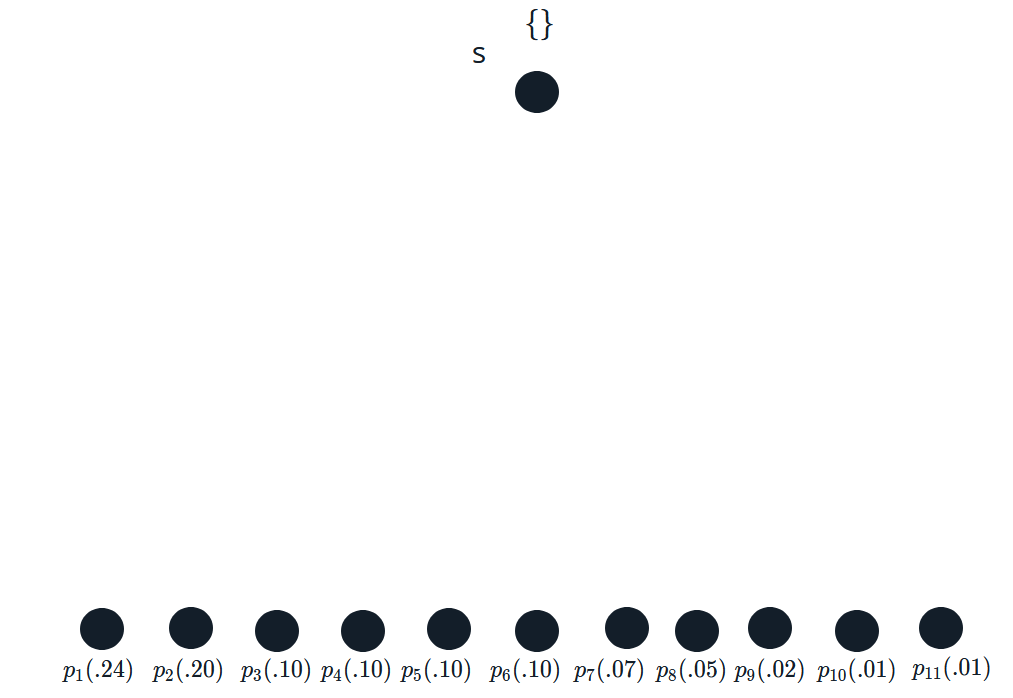
\includegraphics[width=0.49\linewidth]{pictures/huffman2.png}
		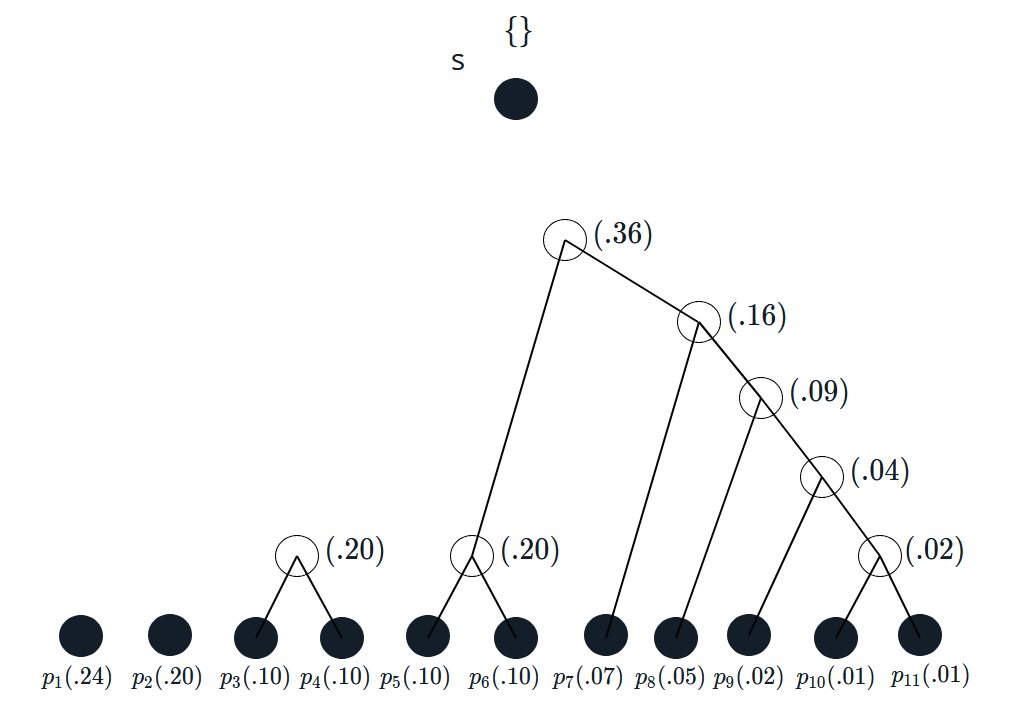
\includegraphics[width=0.49\linewidth]{pictures/huffman3.png}
		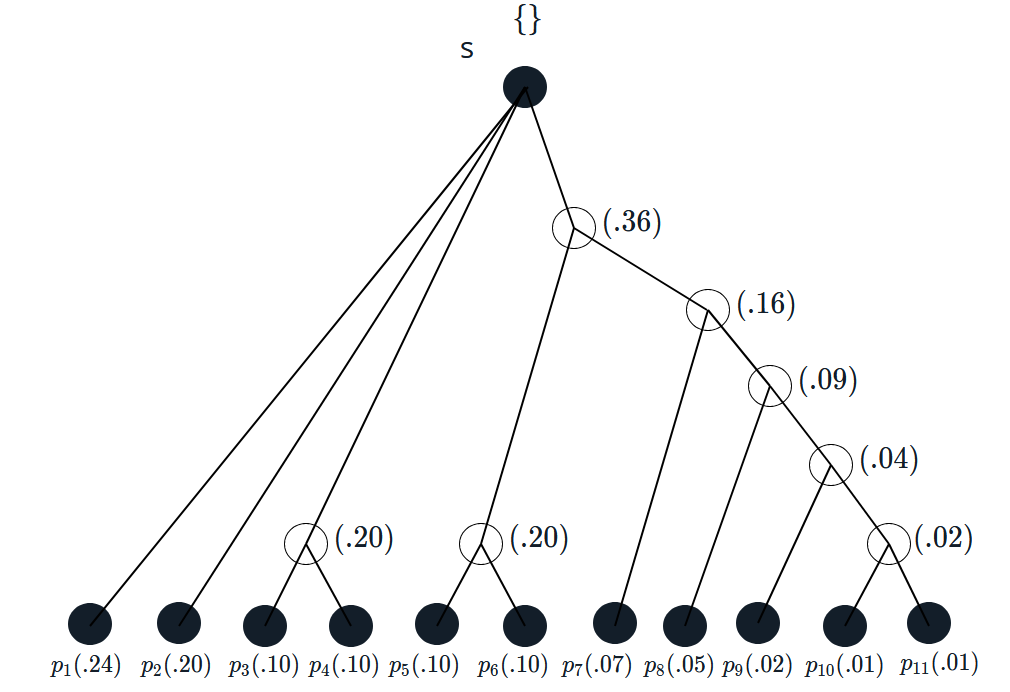
\includegraphics[width=0.49\linewidth]{pictures/huffman4.png}
		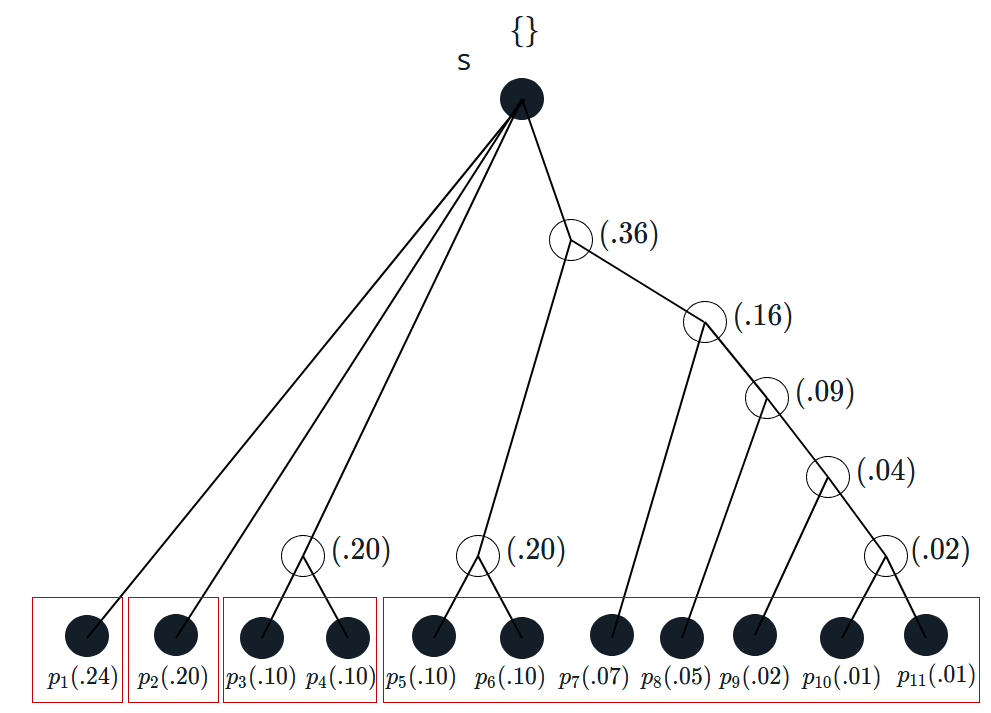
\includegraphics[width=0.49\linewidth]{pictures/huffman5.png}
		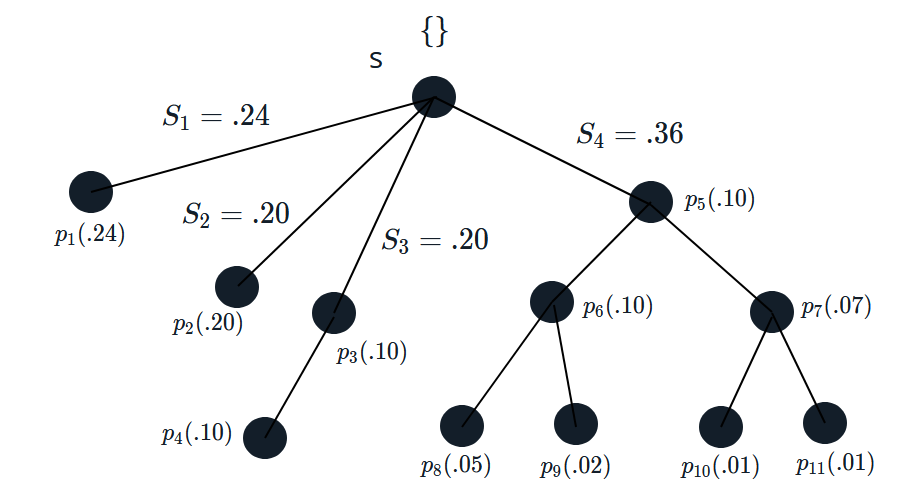
\includegraphics[width=0.49\linewidth]{pictures/huffman6.png}
		\caption{Huffman fa algoritmus lépéseinek vizualizációja a következő valószínűségekre: 
			 \( \{.24, .2, .1, .1, .1, .1, .07, .05, .02, .01, .01\}\) }
		\label{huffman-algorithm}
	\end{center}
\end{figure}


\subsection{Sorfolytonos fa}

Mint láthattuk korábban a Huffman fa alapú algoritmusnál, a levelek felfelé mozgatását sorfolytonosan valósítottuk meg. A sorfolyonos fa is hasonló elvet követ.
Lényegi különbség a kettő fa között, hogy a Huffman kódolási algoritmust kihagyjuk, és egyenest sorfolytonosan rakjuk fel csúcsokat a fa építésekor.
Ezzel mindig a legkisebb fákat kapjuk, de ez a torlódást egyáltalán nem veszi figyelembe.

\subsubsection{Sorfolytonos fa algoritmus}
\begin{itemize}
	\item Végezzük el a fa építés lépésig a cl-Dan algoritmust, demand mátrix itt már a megváltozott állapotban van, nincs két magas csomópont között direkt kapcsolat
	\item Építsük meg a fákat a következő módon:
	\begin{enumerate}
		\item Vegyük a gyökérhez kapcsolódó csúcsok valószínűségét egy vektorba
		\item Rendezzük a vektort csökkenő sorrendbe
		\item Építsünk teljes fát, ahol $\Delta$ csomópont kapcsolódik a gyökér elemre
	\end{enumerate}
\end{itemize}

\begin{figure}[H]
	\begin{center}
		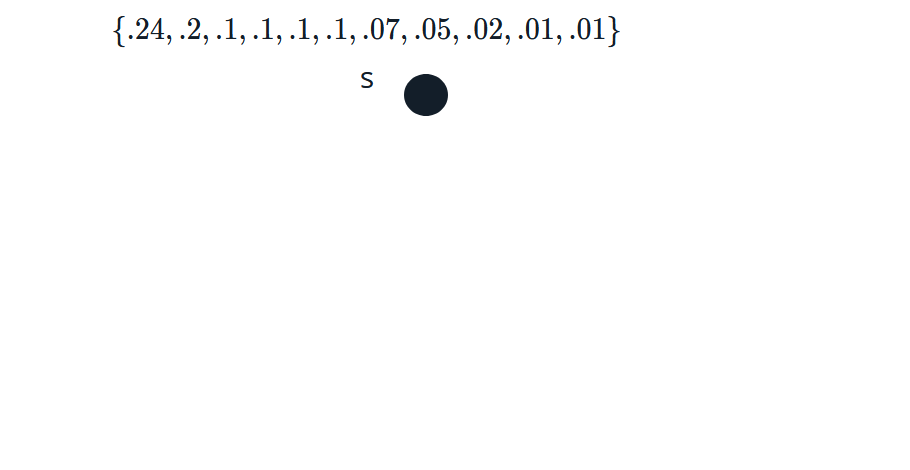
\includegraphics[width=0.49\linewidth]{pictures/bfs1.png}
		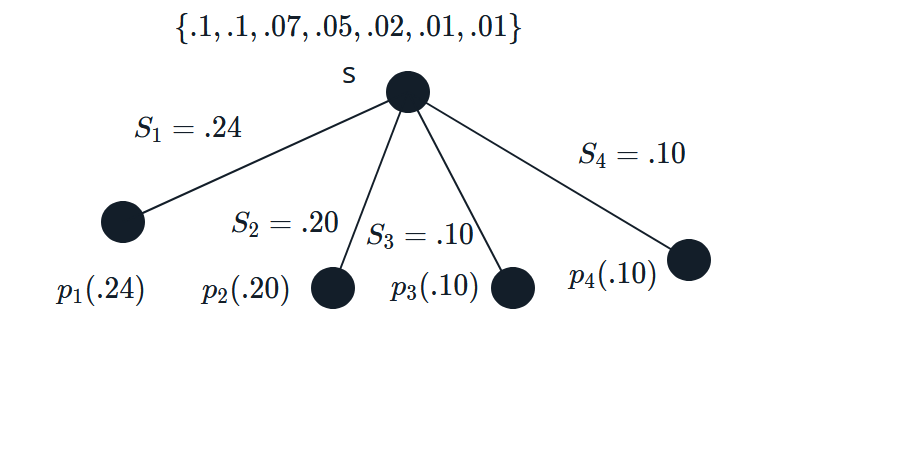
\includegraphics[width=0.49\linewidth]{pictures/bfs2.png}
		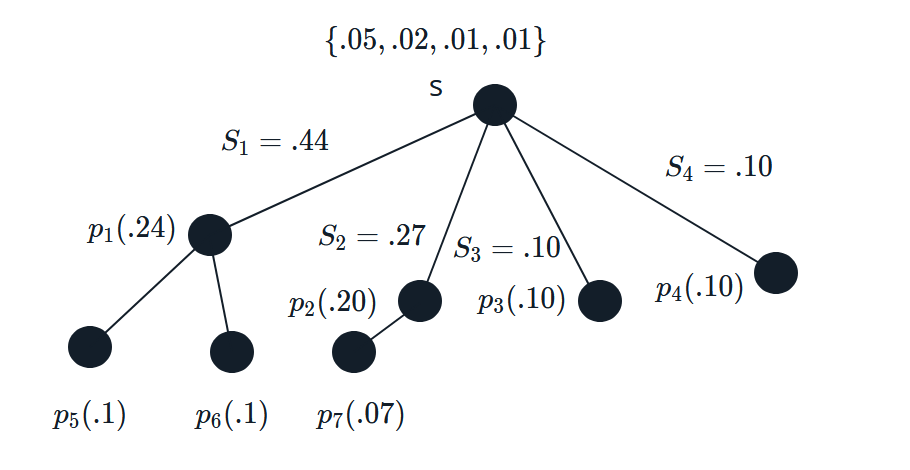
\includegraphics[width=0.49\linewidth]{pictures/bfs3.png}
		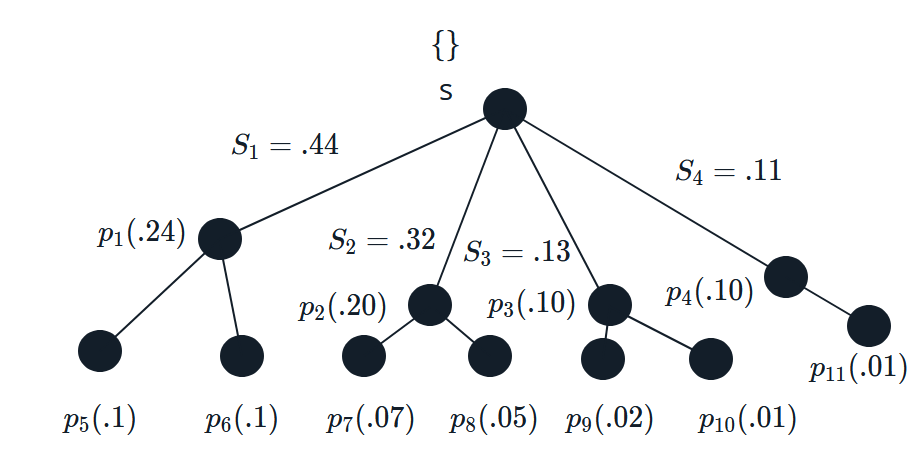
\includegraphics[width=0.49\linewidth]{pictures/bfs4.png}
		\caption{Sorfolytonos algoritmus lépéseinek vizualizációja a következő valószínűségekre: 
			\( \{.24, .2, .1, .1, .1, .1, .07, .05, .02, .01, .01\}\)}
		\label{bfs-algorithm}
	\end{center}
\end{figure}



\subsection{Random fa}

Az eddigi fa építési stratégiák mindegyike valamilyen szempontból próbált egy jobb fát eredményezni.
A Random fa olyan megközelítést használ, hogy szimulálja azt, ha valaki véletlenszerűen kötögetné össze a csomópontokat.
Az így létrehozott fá nem használ semmi olyan információt ami hatékonyabb eredményhez vezetne.
Az algoritmus a már korábban használt Sorfolytonos fára épít, azaz a csomópontokat sorfolytonosan helyezzük el.
Egyetlen változás az algoritmusban, a fához tartozó vektor ami tartalmazza a kommunikációs valószínűségeket nincs sorba rendezve, hanem ötször meg vannak benne keverve az elemek. 

\subsubsection{Random fa algoritmus}
\begin{itemize}
	\item Végezzük el a fa építés lépésig a cl-Dan algoritmust, demand mátrix itt már a megváltozott állapotban van, nincs két magas csomópont között direkt kapcsolat
	\item Építsük meg a fákat a következő módon:
	\begin{enumerate}
		\item Vegyük a gyökérhez kapcsolódó csúcsok valószínűségét egy vektorba
		\item Keverjük össze a vektor elemeit
		\item Építsünk teljes fát, ahol $\Delta$ csomópont kapcsolódik a gyökér elemre
	\end{enumerate}
\end{itemize}

\section{Módosított fa építés}


A cikkben \cite{avin_demand-aware_nodate} szereplő cl-DAN algoritmus első lépése a csomópontok besorolása magas és alacsony halmazokba a fokszámuk alapján. 
A szerzők itt fele-fele arányban osztják el a pontokat és egy hozzáadott feltételként megnézik, hogy az alacsony fokszámúak között szerepel-e olyan csomópont, aminek a fokszáma meghaladja \(2\rho\)-t, azaz a kétszeres átlag fokszámot.

A általam módosított cl-DAN algoritmus ezt a kiegészítő szabályt veszi alapul.
Mi lenne ha, nem szabályosan fele-fele arányba lenne elosztva, hanem magán a \(2\rho\) feltételen?

Nézzünk egy példát, ahol ez jelentőséggel bír.
Tegyük fel, hogy van egy 25 csúcsú csillaggráfunk két csillaggal.
A csillaggráfban a csillag közepére kapcsolódik rá az összes másik csomópont, így van kettő 24 fokú csomópontunk, és huszonhárom darab 2 fokú csomópont. 
Az átlag fokszám így \(\rho=23\cdot2+2\cdot23=3.68\), ennek a kétszerese \(2\rho=7.36\).

Az eredeti esetben a nagy fokú csomópontokhoz a csillagok közepei fog tartozni és további tizenegy darab 2 fokú csomópont. 
Így legalább $\lceil\frac{n}{2}\rceil$ fát fogunk építeni, ahol a pontok nagy része olyan kapcsolatban van, hogy két 2 fokszámú között egy segítő csúcs van, ami hasonló hozzájuk és eredetileg 2 fokszámú volt. 
Ezzel a módszerrel jelentősen növeltük meg a torlódást a gráfban.

A módosított algoritmus az eredetivel ellenben a magas halmazban csak két darab csúcsot tartalmaz, a középpontokat.
Ezen esetben ténylegesen magas csomópontok közé helyezünk egy kisegítőt, ami bármelyik lehet a maradék 2 fokszámú csúcsok közül, ezzel redukáltuk is az épített fák számát.
%A torlódásra tekintette, meg azt tapasztalhatjuk, hogy kevesebb lesz, mintha az eredeti módszer segítségével csináltuk volna. 

A módosított algoritmus nem lesz rosszabb mint az eredeti algoritmus, mivel ott mit kiegészítő feltétel szerepel a fokszám ellenőrzés, még itt az alapot adja, így legrosszabb esetben is visszatérünk az eredetihez. 

\chapter{Megvalósítás}


\section{Keretrendszer}

A keretrendszer Python 3 \cite{noauthor_python_nodate} nyelven íródott és a Networkx \cite{noauthor_networkx_nodate} külső csomag volt használva a véletlen gráfok generálására.
A példakód megtalálható futtatható hagyományos Python programként és Jupyter notebookban \cite{noauthor_jupyter_nodate}.  
Networkx csomag továbbá biztosít számunkra egy megjelenítési lehetőséget, amit a Jupyter notebookban tudunk legjobban kihasználni.
Az adatok feldolgozása és kiértékelése is Jupyter notebookban történt. 

\section{Adatszerkezetek}

A modell alapját pár egyszerű alaptípus adja. Ezek rendre a következők:
\begin{itemize}
	\item \textbf{Vertex} - az általános gráf csúcs
	\item \textbf{Node} - az \textit{Egófák} készítésekor használt csúcs, ami tartalmazza a valószínűségét annak, hogy a forrás csomópont mekkora valószínűséggel fog kommunikálni a másik \textit{Node} csúccsal
	\item \textbf{HuffmanDanNode} - a Huffman fa csomópontjait reprezentáló osztály, minden tulajdonsága megvan mint a Node-nak, csak még kiegészül egy útvonallal, ami a Huffman fa építése után lesz meghatározva
	\item \textbf{Edge} - a gráf pontjait összekötő él reprezentációja, ami \textit{Vertexet} vár paraméterként, és tartalmazza a kommunikációs valószínűséget, hasonlóan mint a \textit{Node}
	\item \textbf{Tree} - ami adja az alapját majd a útvonal tervezési sémának. A fának két fajtája van megvalósítva:
	\begin{itemize}
		\item \textbf{EgoTree} - a $\Delta$ fokú Egófa, ahol a gyökérnek legfeljebb $\Delta$ levele lehet
		\item \textbf{HuffmanDanTree} - a $\Delta$ fokú Huffman fa, ahol a gyökérnek legfeljebb $\Delta$ levele lehet és a belső csúcsok állhatnak üresen
	\end{itemize}
	
	
\end{itemize}

\section{Hálózat modell}

A \textbf{Network} osztály valósítja meg az algoritmus legnagyobb részét, de magában nem használható, mivel nem tartalmazza a fa építési stratégiát.
Ahhoz, hogy a teljes legyen az osztály, le kell származtatni és meg kell valósítani milyen algoritmussal építse meg a fákat.
Ennek segítségével nagyon egyszerűen lehet új algoritmust illeszteni a már meglévő rendszerhez.

A Network osztály bemenete a demand mátrix, kimenete egy útválasztási séma.
Az algoritmus futtatásához szükség van még egy paraméterre, ahol megadjuk a maximális fokszámot a rendszernek, ami alapján elkészülnek a fák.
Itt kettő lehetőségünk van, kötött és dinamikus fokszám, attól függően mit szeretnénk elérni.
A dinamikus fokszám esetén az átlag fokszám függvényében lehet megadni a maximális fokszámot.
Erre egy példa a "6d", ahol azt fejezzük ki, hogy az átlag fokszám hatszorosát szeretnénk használni az adott gráfban, mint maximális fokszám a megépítendő fák esetén.
Az útválasztási séma létrehozásakor a csere lépéssorozatot követően megváltozik a demand mátrix, ezért fontos, hogy a \(\Delta\) fokszámot ne haladjuk meg, de ez nem garantált.
Az algoritmus kimenete mellett további metaadatok tartalmazzák a kiszámított maximális $\Delta$ fokszámot és a valós fokszámot.
A valós fokszám adja azt a fokszámot amire algoritmusnak tényleg szüksége volt.  
Ezekből az adatból lehet következtetést levonni, hogy valóban megfelelő-e a felső korlátja az algoritmusnak, amit a szerzők adtak és lehetőséget ad egy jobb felső korlát becslésre. 


Az algoritmushoz szükséges bemeneti demand mátrix több módos is megadható konfiguráción keresztül.
A konfigurációk egy  \textit{JSON} fájl tartalmazza, amiben egyszerre több konfiguráció is megadható. 
A lehetséges konfigurációk pedig a következők módon adhatók meg.

Először is, van lehetőségünk egy konkrét mátrixra elkészíteni az útválasztási sémát.
Egy így megadott helyes konfiguráció pedig a következő:

\pagebreak

\begin{mintedJson}
	{
		"config": [
		{ 
			"graph": "manual",
			"dan": 3,
			"demand": [
			[0, 3, 4, 1, 1, 1, 1],
			[3, 0, 2, 0, 1, 0, 4],
			[4, 2, 0, 2, 0, 0, 4],
			[1, 0, 2, 0, 3, 0, 0],
			[1, 1, 0, 3, 0, 0, 0],
			[1, 0, 0, 0, 0, 0, 3],
			[1, 4, 4, 0, 0, 3, 0]]	
		} ]
	}
\end{mintedJson}

Fontos paraméterek az ilyen konfiguráció esetén a következők:
\begin{itemize}
	\item $graph$ - itt adjuk meg a bemeneti gráf típusát, esetünkben ez $"manual"$, azaz ezt a megadott mátrixot fogja használni az algoritmus.
	\item $dan$ - ez a paraméter határozza meg a maximum fokszámot a magas fokú csomópontokra, itt megadható konkrét érték pl. 3, dinamikus érték pl. $"6d"$ vagy $null$ ami ekvivalens a $"12d"$ értékkel, ami a cikkben \cite{avin_demand-aware_nodate} meghatározott felső korlát.
	\item $demand$ - maga a demand mátrix, listák listájaként egy négyzetes mátrix, ahol a diagonális elemek értéke $0$, mivel önmagával való kommunikáció nem befolyásolja a hálózatot
\end{itemize}

A konkrét demand mátrix megadás mellett van még lehetőség generálni véletlen gráfot.
A program három fajta véletlen gráf típust tud generálni, amik rendre: Barabási-Albert gráf, Erdős-Rényi gráf és csillaggráf.

A véletlen gráfok konfigurációit meg lehet adni hasonló módon mint az előző esetben.
Több konfiguráció megadása a $config$ tömbben vesszővel elválasztva történik.
A véletlen gráfok konfigurációja megegyezik, és a gráf típusától függően változik a konstans jelentése. 
Egy példa erre a következő kód részlet:

\pagebreak

\begin{mintedJson}
{
	"graph": "star",
	"vertex_num": 25,
	"constant": 1,
	"dan": 10
}
\end{mintedJson}


A paraméterek rendre a következők:

\begin{itemize}
	\item $graph$ - véletlen gráf típusa, aminek a lehetséges értékei:
	\begin{itemize}
		\item $"barabasai-albert"$ - Barabási-Albert gráf
		\item $"erdos-renyi"$ - Erdős-Rényi gráf
		\item $"star"$ - Csillaggráf
	\end{itemize}
	
	\item $vertex\_num$ - Csomópontok száma
	\item $dan$ - A maximális fokszám a magas fokú csúcsokra, megegyezik az előző esettel
	\item $constant$ - Konstans érték ami a megadott gráf paraméterét adja, ezek rendre a következők:
	\begin{itemize}
		\item Barabási-Albert gráf esetén a "preferential attachment" számát adja meg
		\item Erdős-Rényi gráf esetén az él valószínűségét határozza meg a következő képlet segítségével:  \[p = \frac{constant}{vertex\_num}\]
		\item Csillaggráf esetén pedig a csillagok számát adjuk meg
	\end{itemize}
\end{itemize}


\section{Kimenet}

Az program kimenete, az algoritmus által kiszámolt metrikák köztük az átlag súlyozott úthossz és a torlódás. 
Ha a rajzolás opció be van kapcsolva, akkor a kiindulási hálózat, az egófák és az új hálózat 
útválasztási sémája lesz kirajzolva.

\begin{figure}[H]
	\begin{center}
		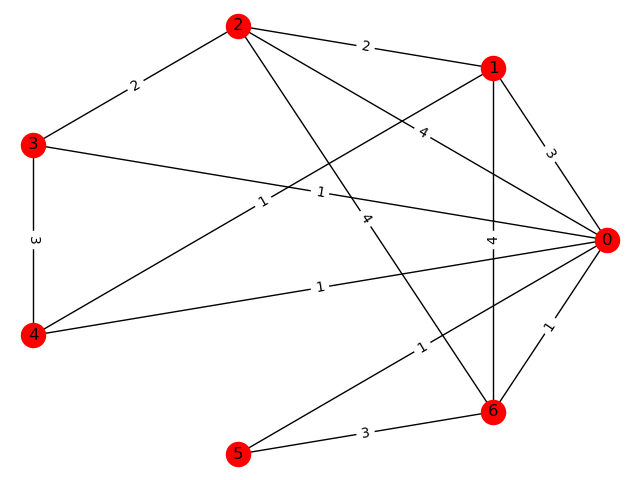
\includegraphics[width=0.49\linewidth]{pictures/starting_network.png}
		\caption{Kiindulási hálózat}
		\label{starting-network}
	\end{center}
\end{figure}

A \ref{starting-network} ábrán látható a bemeneti hálózat, aminek a demand mátrixa már a korábban fel lett írva. Az algoritmus ezek után a cl-DAN algoritmust használva, először elkészíti az egófákat \ref{ego-trees} ábra, majd végül az új hálózat választási sémát ami a \ref{routing-scheme} ábrán látható.

\begin{figure}[H]
	\begin{center}
		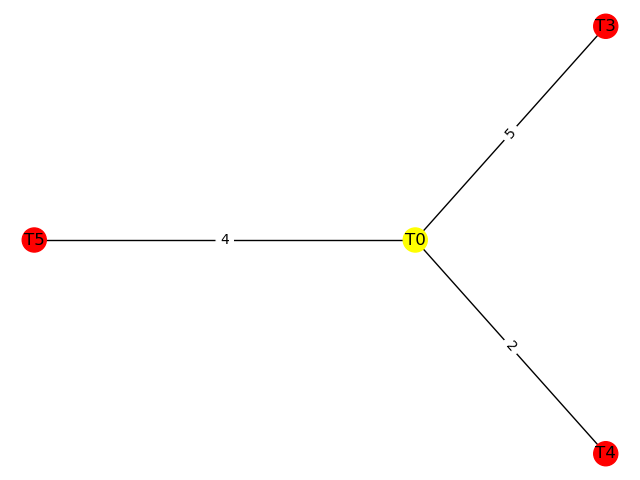
\includegraphics[width=0.40\linewidth]{pictures/egotree1.png}
		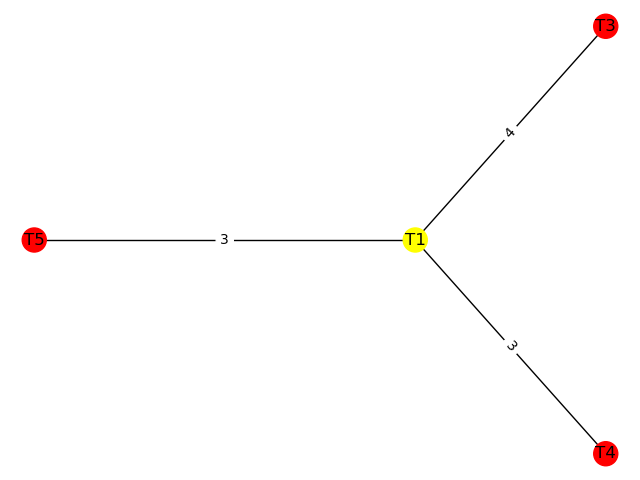
\includegraphics[width=0.40\linewidth]{pictures/egotree2.png}
		%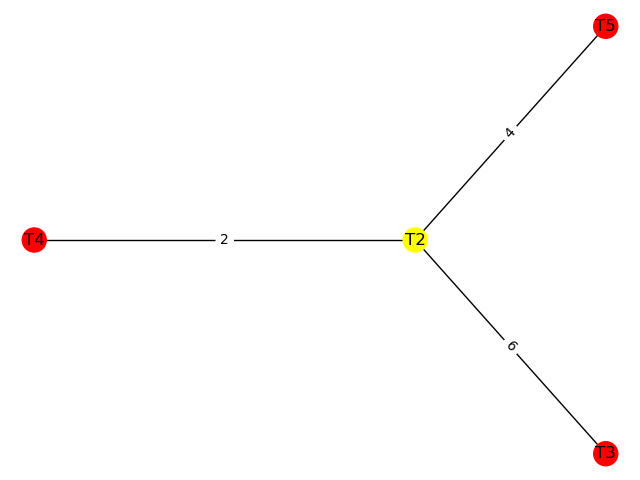
\includegraphics[width=0.40\linewidth]{pictures/egotree3.png}
		%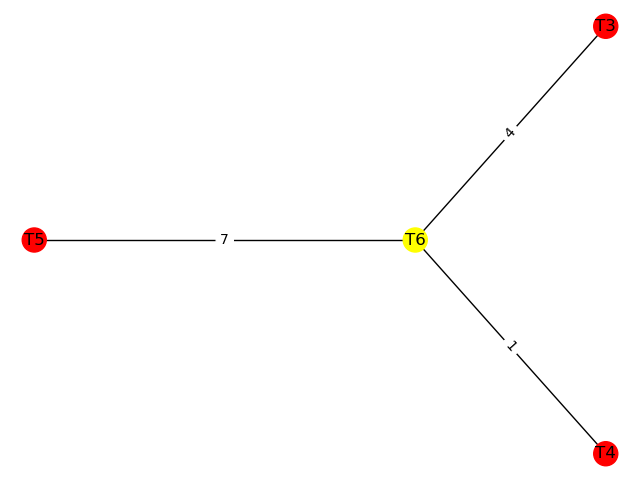
\includegraphics[width=0.40\linewidth]{pictures/egotree4.png}
		\caption{Egófák}
		\label{ego-trees}
	\end{center}
\end{figure}

A \ref{routing-scheme} ábrán látható gráfon pár extra információ megfigyelhető. 
Pirosra vannak festve a magas fokszámú csúcsok és zöldre az alacsony fokszámúak.
Az algoritmus fő célja az volt, hogy ne legyen egymással közvetlen kapcsolatban két magas fokszámú csúcs, azaz ne legyen két piros csúcs összekötve, és ez maradéktalanul teljesül is.
Két magas fokszú csúcs csak egy alacsony fokszámú segítő csúcson keresztül tud kommunikálni.
Fokszámok szempontjából a csúcsok rendben vannak, mivel nem haladják meg $\Delta$ fokszámot. 
A gráf esetén a delta \(\Delta = 12\rho = 12 \cdot \lceil\frac{25}{7}\rceil = 43  \).

\begin{figure}[H]
	\begin{center}
		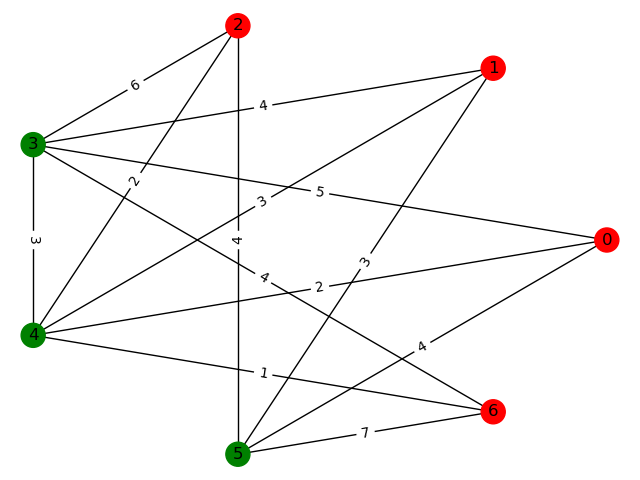
\includegraphics[width=0.49\linewidth]{pictures/new_network.png}
		\caption{Új hálózat}
		\label{routing-scheme}
	\end{center}
\end{figure}

Egy érdekes tény még megfigyelhető a \ref{routing-scheme} gráfon, mint a konfigurációnál is említve volt, azoknak a csomópontoknak adjuk meg a maximális fokszámát, ami a magas fokszámúak halmazába fog kerülni. 
Mivel a cl-DAN utolsó lépésében meg van említve, hogy nem csak magas-magas és magas-alacsony kapcsolatok között van él, hanem az alacsony-alacsony között is.
Ez annyiban hat ki a végső útválasztási sémára, hogy ha van két telített segítő pontunk, akkor ellenőrzés nélkül be kell húzni az alacsony-alacsony kapcsolatot, ezzel megszegve azt a feltételt, hogy egy csomópontnak csak meghatározott $\Delta$ fokszáma lehet.
Ha $\Delta$ nagyon kicsi, akkor ez a probléma hatványozottan érvényesül, de ha választunk egy megfelelően nagy és reális fokszámot, akkor ez a probléma nagy valószínűséggel nem fog fellépni.
	


\chapter{Tesztelés}


\section{Tesztelés menete}

A megfelelő teszt mennyiség eléréséhez véletlen gráfok lettek generálva. 
Mind a három gráf típus lett tesztelésre használva, ezek paramétere pedig változott egy és tíz között.

A különböző kapacitás szimulálására a maximum fokszám meg lett határozva, hogy a 
következő halmaz elemit veheti fel $\Delta\in[10, 16, 24, 48]$.
A tesztek segítségével ki lett mutatva, hogy egy ponton túl, már annyira nagy lesz a $\Delta$ értéke dinamikus esetben, hogy minden csúcs a gyökérre kapcsolódik.
Ezzel teljesen értelmét vesztve, hogy milyen fa építési stratégia volt használva, mivel a fa nem éri azt az elemszámot, hogy legyen nem direkt csatlakozó csomópont a gyökérhez. 
A \ref{delta} ábrán látható ez:  

\begin{figure}[H]
	\begin{center}
		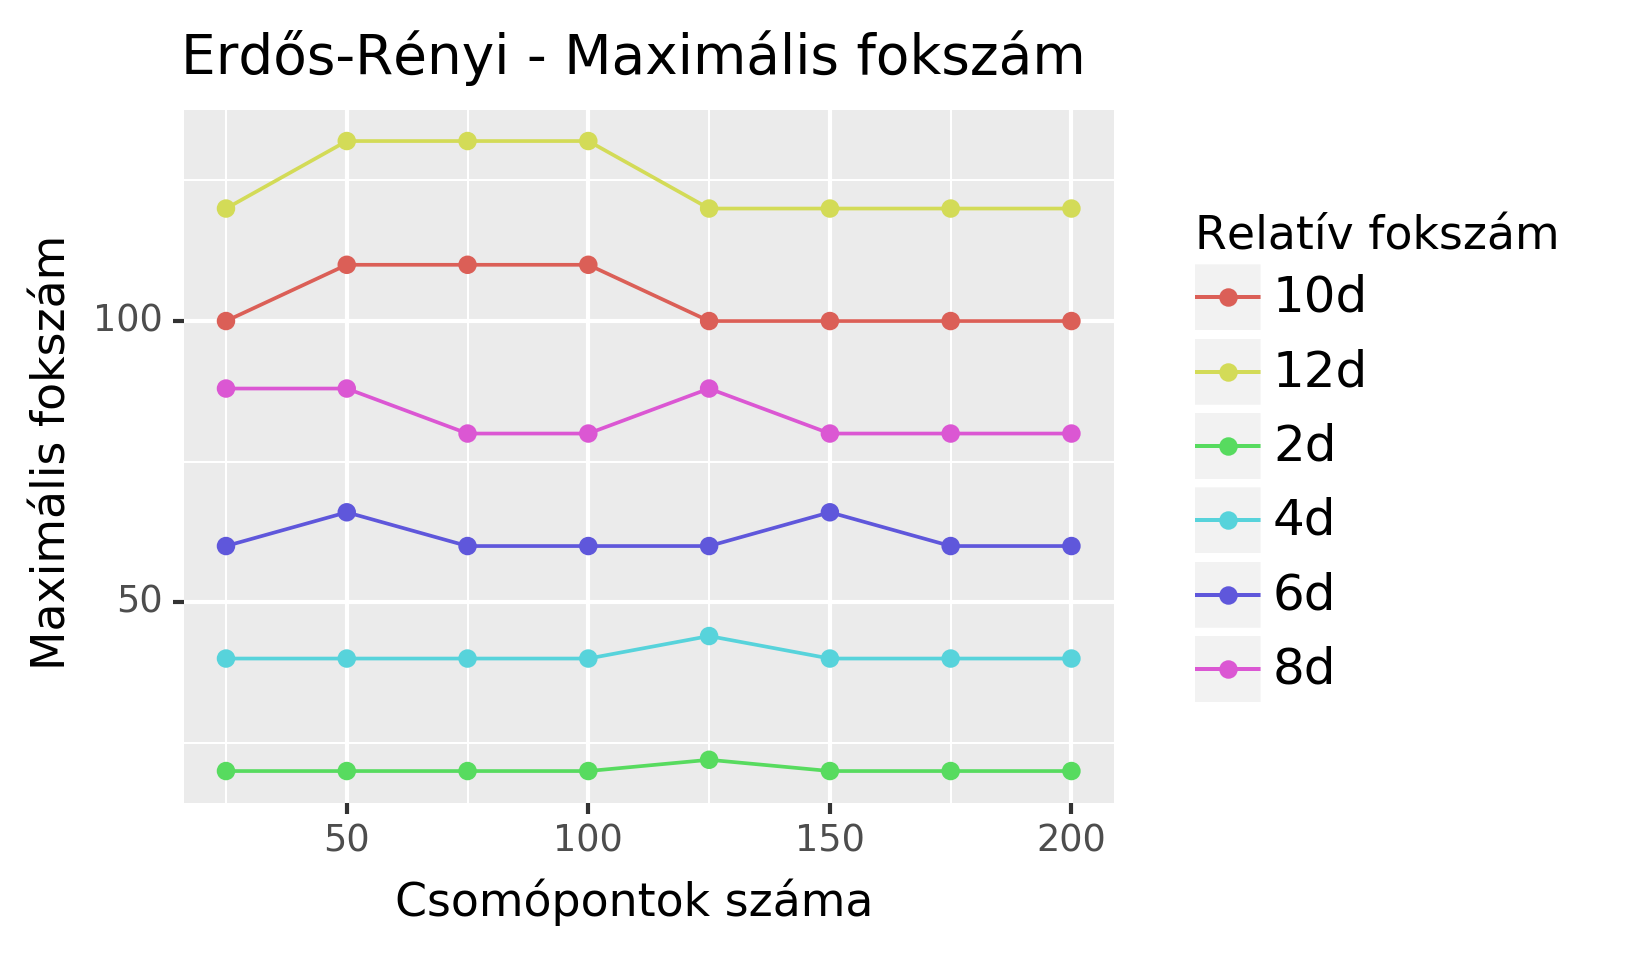
\includegraphics[width=0.49\linewidth]{pictures/delta_max.png}
		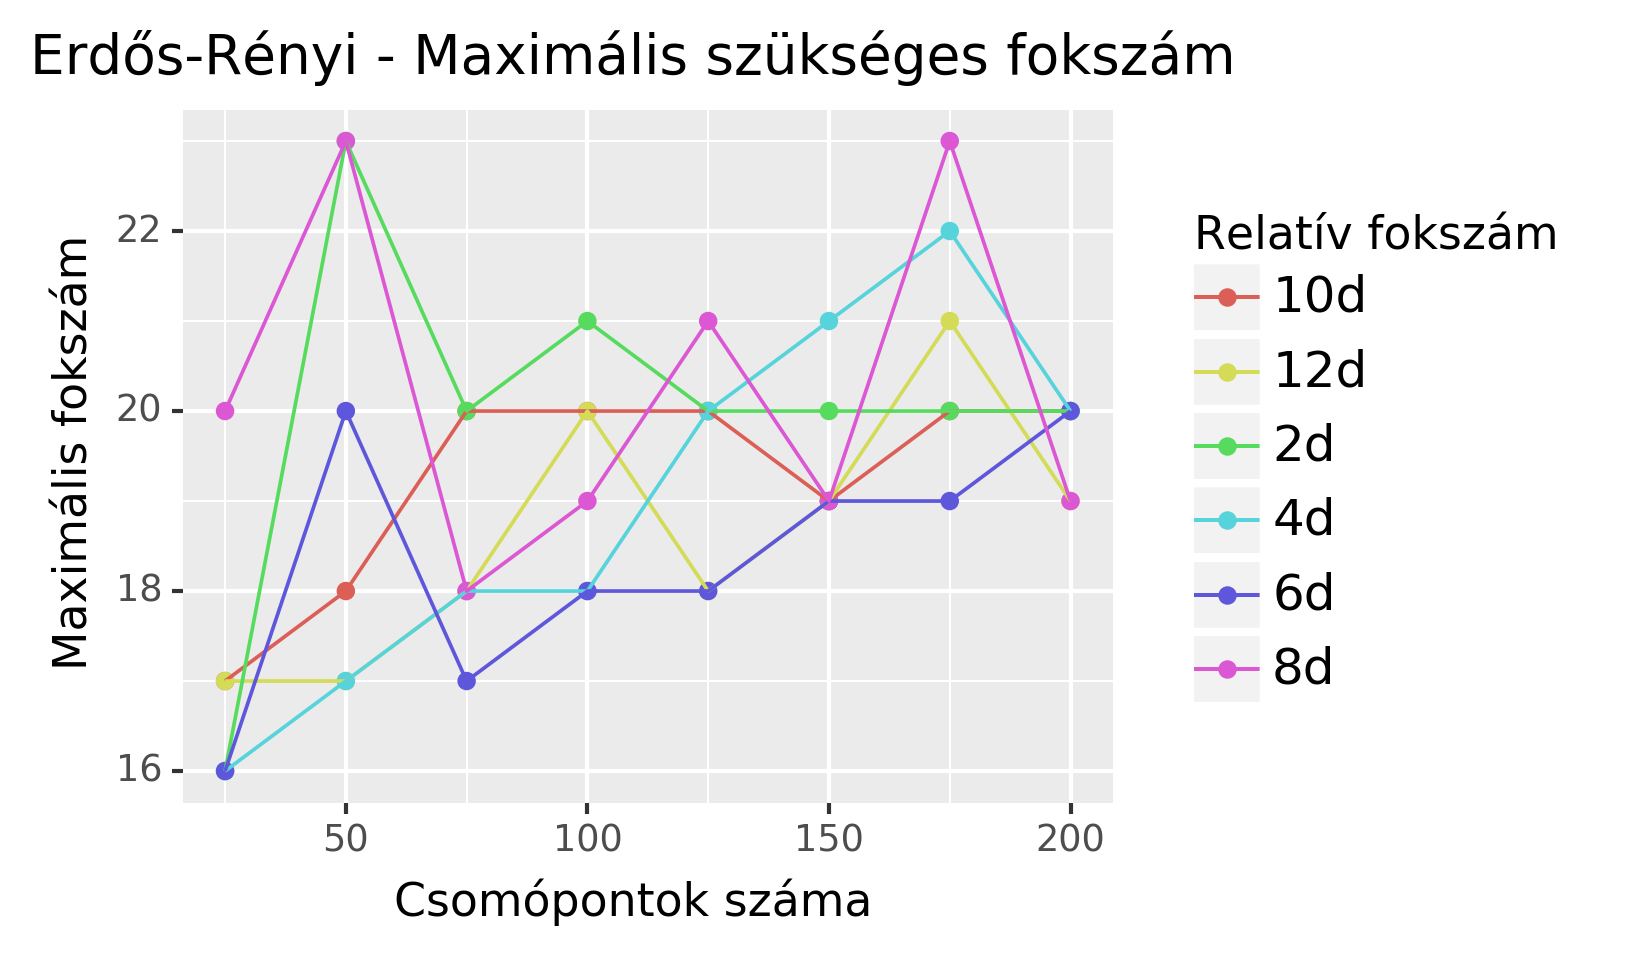
\includegraphics[width=0.49\linewidth]{pictures/delta_req.png}
		\caption{Erdős-Rényi gráf - Fa mennyiség összehasonlítás}
		\label{delta}
	\end{center}
\end{figure}

A következő szempont amiben változtak a gráfok, hogy mekkora terhelés legyen az éleken.
Itt két csoportba lehet sorolni a teszteket, ahol egytől tízig véletlenszerűen volt kiválasztva, a második esetben pedig minden él egységesen egy terhelést kapott.

Következő szempont amit figyelve volt az maga az algoritmus változtatása, hogy mennyi fa készüljön el, és hogy milyen stratégiával.

Végül pedig, hogy a mérési hiba minimalizálásának érdekében az fent említett paraméterek összes kombinációjára húsz teszt futott le. 
Összességében 384.000 teszt készült le, amit meg lehet találni a projekt GitHub oldalán.

\section{Metrikák}

Tesztek különböző metrikák alapján lettek kiértékelve, amik a következők:

\begin{itemize}
	\item $graph$ - gráf típusa 
	\item $vertex\_num$ - csúcsok száma a gráfban
	\item $constant$ - a gráfhoz tartozó konstans paraméter 
	\item $congestion$ - torlódás az eredeti értékekkel
	\item $real\_congestion$ - a torlódás normalizálva egyre
	\item $avg\_route\_len$ - átlag úthossz
	\item $delta$ - fa $\Delta$ fokszáma
	\item $max\_delta$ - a maximális $\Delta$ fokszám
	\item $dan$ - a $\Delta$ megadott fokszám, ami lehet relatív is
	\item $most\_congested\_route$ - a legnagyobb torlódással rendelkező él
	\item $max\_route\_len$ - a maximális úthossz
	\item $avg\_tree\_weight$ - az átlag fa súlya
	\item $most\_tree\_ratio$ - a legnagyobb arány fa átlag ágsúlya és a legnehezebb ág között
	\item $tree\_count$ - az épített fák száma
	\item $type$ - a fa építései algoritmus típusa
	\item $start\_entropy$ - a kezdeti költség mátrix entrópiája
\end{itemize}
	

\chapter{Teszt eredmények kiértékelése}

\section{Entrópia}

A különböző gráf típusok különböző entrópiával rendelkeznek.
Az entrópia diszkrét valószínűségi változóra felírható a következő képlettel \cite{DBLP:journals/corr/AvinMS17}:  

\[H(X) = \sum_{i=1}^{n} p(x_i) \cdot log_2\frac{1}{p(x_i)}; \; \forall i\in[1, ..., n] \land x_i = \sum_{1}^{n} demaind\_matix[i][n]\] 

Megjegyzés: mikor \(0\cdot log_2\frac{1}{0}\) értéket vesz fel az \(x_i\) változó, akkor legyen \(x_i=0\). 
Legyen \(\bar{p}\) a demand mátrix, ekkor \(H(\bar{p})\) megegyezik a következővel \(H(p_1, p_2, ..., p_n)\), ahol \(p_i\) a mátrix egy sorában szereplő valószínűségek összege.
Ha teljesül, hogy \(p_i > 0\) és $\sum_{i}p_i = 1$ és a \(\bar{p}\) egyenletes eloszlást követ, akkor a véletlen gráfban az entrópiára felső korlátja \(H(\bar{p}) = \log n\), ahol $n$ a csomópontok száma.

A fenti képlet segítségével ki lehet számolni az entrópiát a különböző véletlen gráfokra.
A következő grafikon mutatja, hogy a tesztek során használt véletlen gráfoknak mennyi az entrópiájuk.
Eredmény a \ref{entropy} ábrán.

\begin{figure}[H]
	\begin{center}
		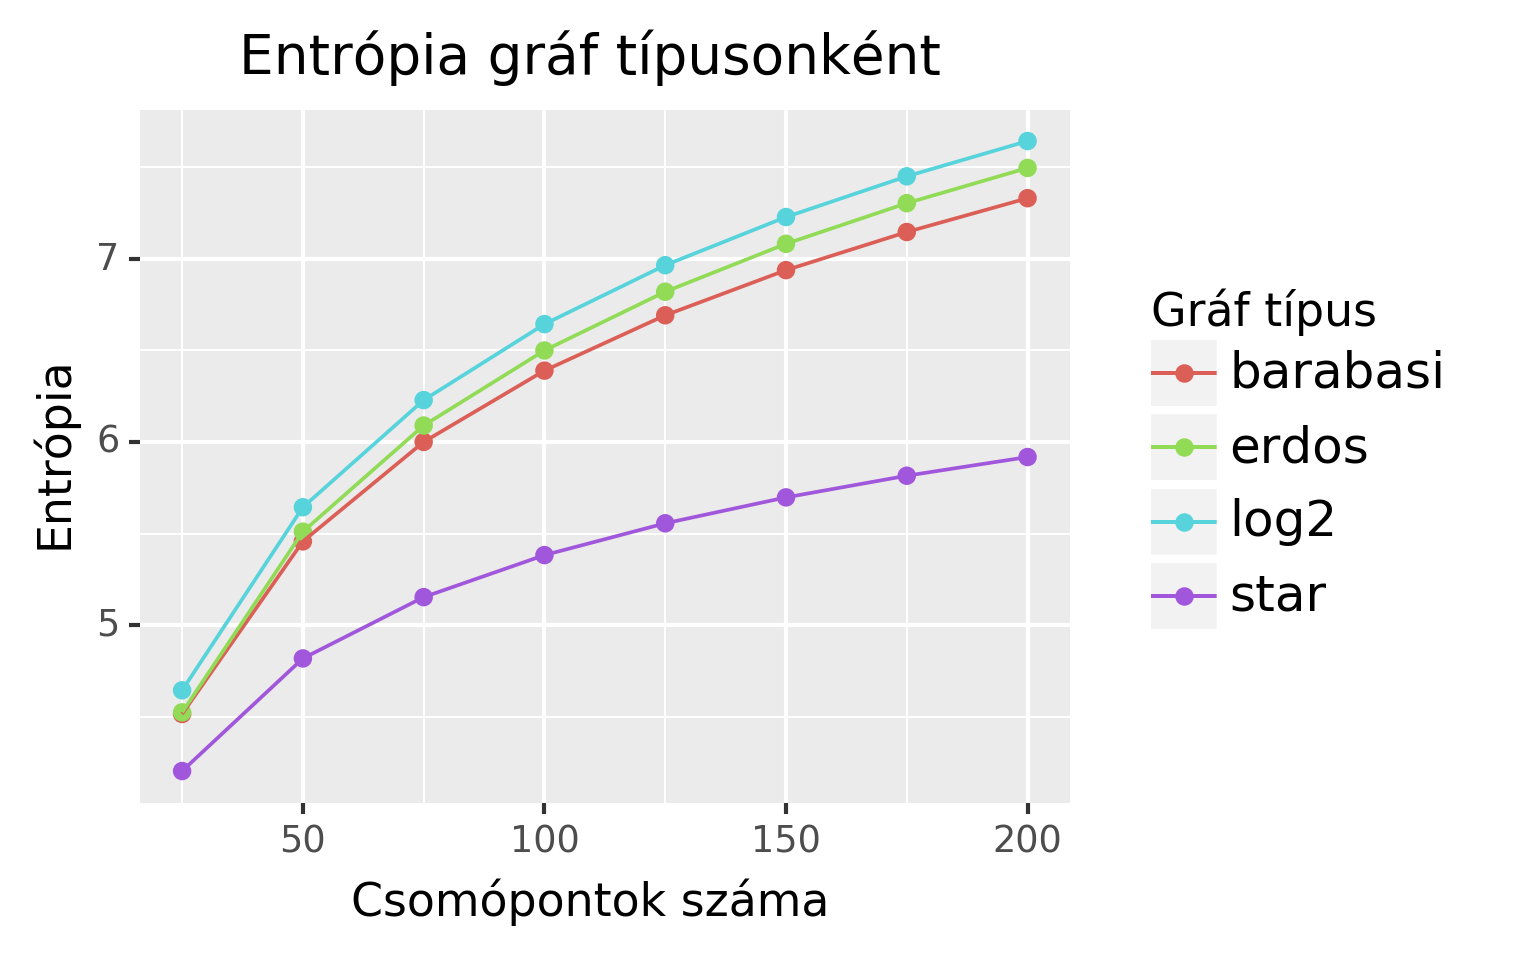
\includegraphics[width=0.9\linewidth]{pictures/entropy.png}
		\caption{Entrópia}
		\label{entropy}
	\end{center}
\end{figure}

A grafikonon látható, hogy az Erdős-Rényi gráfnak van a legnagyobb entrópiája, itt egy valószínűség változó határozza meg mennyi éle lesz a gráfnak.
Ezt követi a Barabási-Albert gráf, ahol tudjuk mennyi élt várunk, annak függvényében mennyi régi csomópontra kell kapcsolódnia az új csomópontnak.
Majd végül a legkisebb entrópiát a csillag eredményezte, mivel a csúcsok csak a csillag középpontokhoz csatlakoznak, máshova nem.
A $\log_2n$ pedig az elméleti felső korlát.
\section{Úthossz}

\subsection{Általános eset}

A tesztek során a konstans érték határozta meg, hogy mennyire volt kitöltve a demand mátrix.
Ezért először nézzük meg mennyire van kihatással a mátrix kitöltöttsége az eredményekre.

Eredmény a \ref{density-len} ábrán.

\begin{figure}[H]
	\begin{center}
		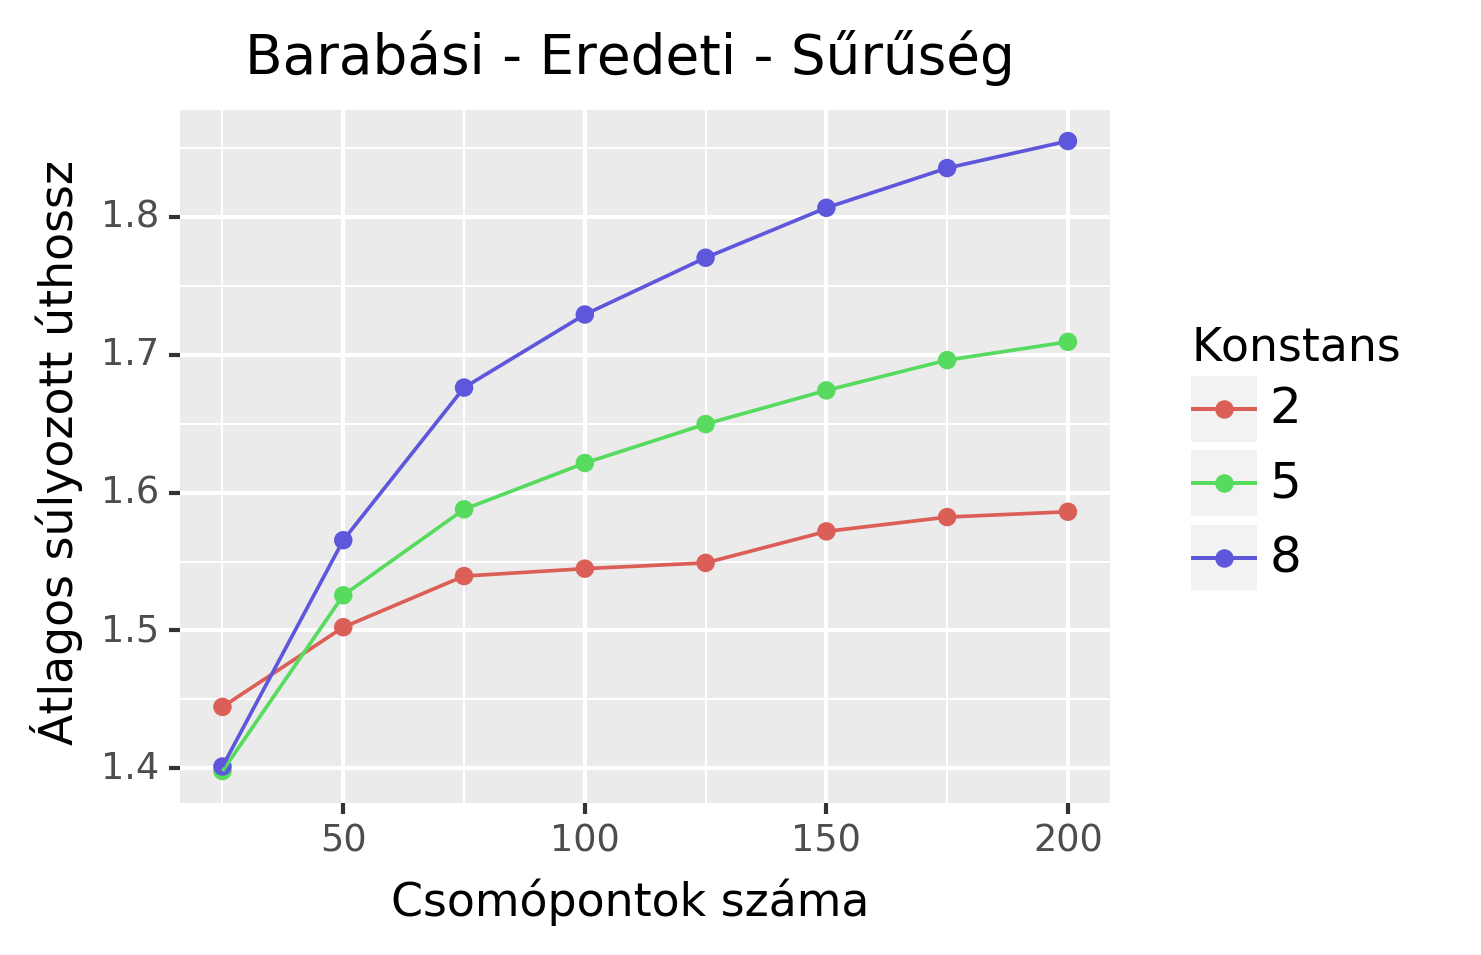
\includegraphics[width=0.9\linewidth]{pictures/density_len.png}
		\caption{Átlagos súlyozott úthossz és demand mátrix kitöltöttségének kapcsolata}
		\label{density-len}
	\end{center}
\end{figure}

A grafikonon a Barabási-Albert gráf eredményei látható, az eredeti mennyiségű fa megépítésével, azaz legalább minden második csúcsponthoz elkészült, és a fák pedig az eredeti algoritmussal készültek el.
A hálózatban az összes szereplő él súlya 1, normalizálás után pedig
\(\frac{1}{|E|}\).
Mint látható a grafikonon, minél ritkább a mátrix, annál rövidebbek az úthosszak is.
A további grafikonoknál már csak a konstans 5 értékű eredményeket fogom vizsgálni, mivel az ad egy jó közelítést az átlagra.

\subsection{A fa építő algoritmusok összehasonlítása}

\subsubsection{Eredeti megépített fa mennyiség}

Az általános esetben csak egy véletlen gráfnak a konkrét esetét néztük meg, most vizsgáljuk meg, hogy a különböző fa építési stratégiák, hogy befolyásolják az úthosszt.

Első véletlen gráf típus a Barabási-Albert gráf, ahol az eredeti számú fát építettük meg. 
Eredmény a \ref{barabasi-len} ábrán.

\begin{figure}[H]
	\begin{center}
		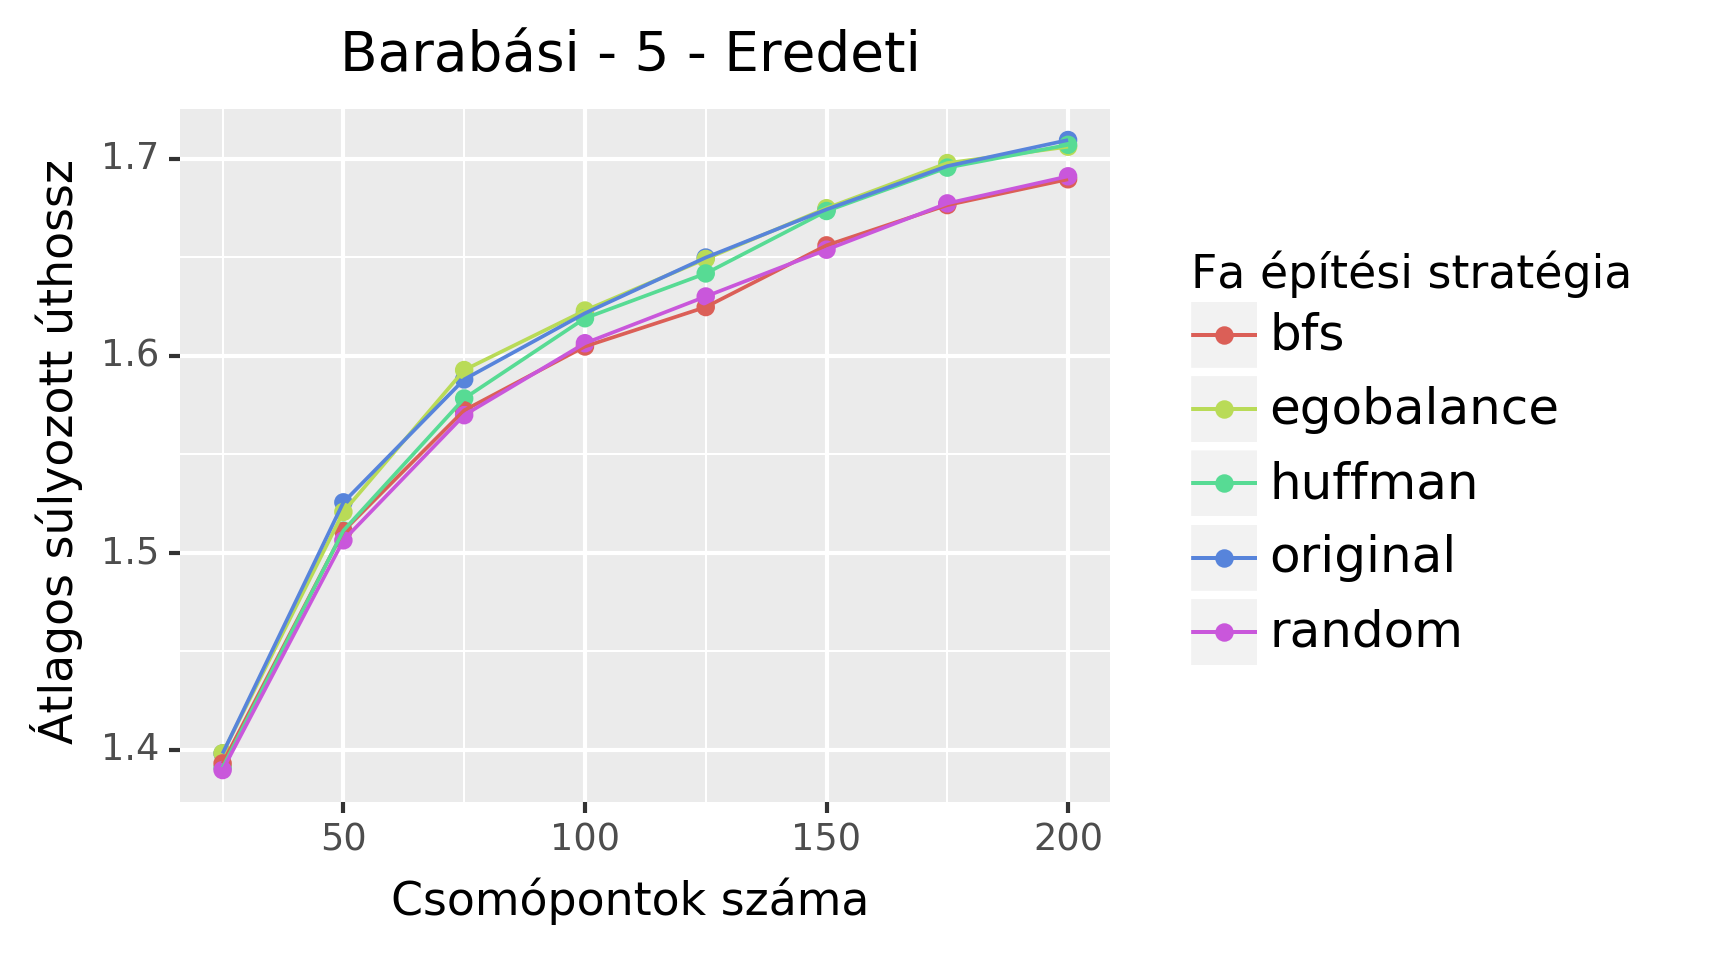
\includegraphics[width=0.9\linewidth]{pictures/barabasi_len_e.png}
		\caption{Barabási-Albert gráf - Úthossz}
		\label{barabasi-len}
	\end{center}
\end{figure}

A grafikonon látható, hogy három csoportba lehet besorolni az algoritmusokat. 
Az elsőbe tartozik az EgoBalance és az Eredeti algoritmus.
Ezek rendelkeznek a legnagyobb átlagos úthosszal és szinte ugyanazt az eredmény adják, mérési hiba különbséggel.
A következő a sorban a Huffman fa alapú algoritmus, ami kezdetben alacsonyabbról indul, de végül csatlakozik az első kettőhöz.
Legjobb két algoritmus pedig a Sorfolytonos fa és a Random fa.
Ez várható volt, mivel mindkettő ugyanazt az algoritmust használja, csak az értékekben különböznek.
Úthossz szempontjából ez a kettő adja mindig legkisebb fát, mivel egy teljes fát épít az algoritmus.


Következő véletlen gráf típus amit vizsgálunk az az Erdős-Rényi gráf, itt is az eredeti számú fát építjük meg.
Eredmény a \ref{erdos-len} ábrán.

\begin{figure}[H]
	\begin{center}
		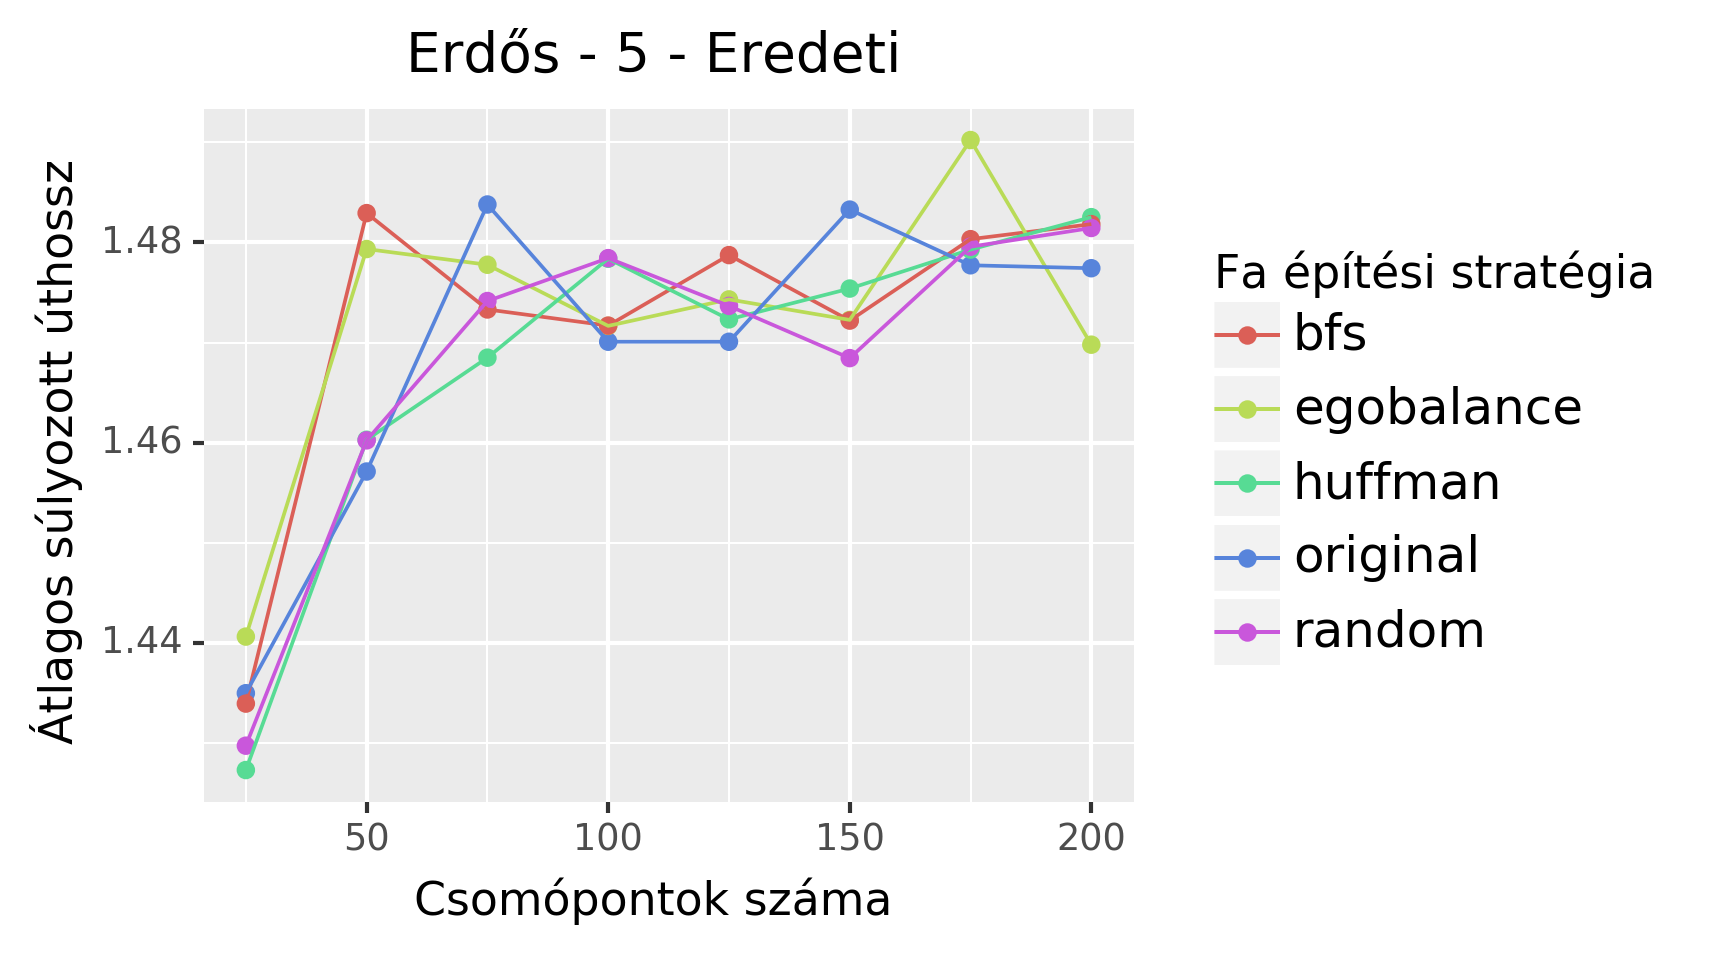
\includegraphics[width=0.9\linewidth]{pictures/erdos_len_e.png}
		\caption{Erdős-Rényi gráf - Úthossz}
		\label{erdos-len}
	\end{center}
\end{figure}

A grafikon itt már kicsit érdekesebb, mivel kicsit nagyobb mozgása van az értékeknek, de ha megnézzük, legfeljebb kettő százalékos eltérés mérhető.
Az összes algoritmus hasonlóan teljesít.   

Végül pedig nézzük meg a csillaggráfot az eredeti számú fa mennyiséggel a \ref{star-len} ábrán.

\begin{figure}[H]
	\begin{center}
		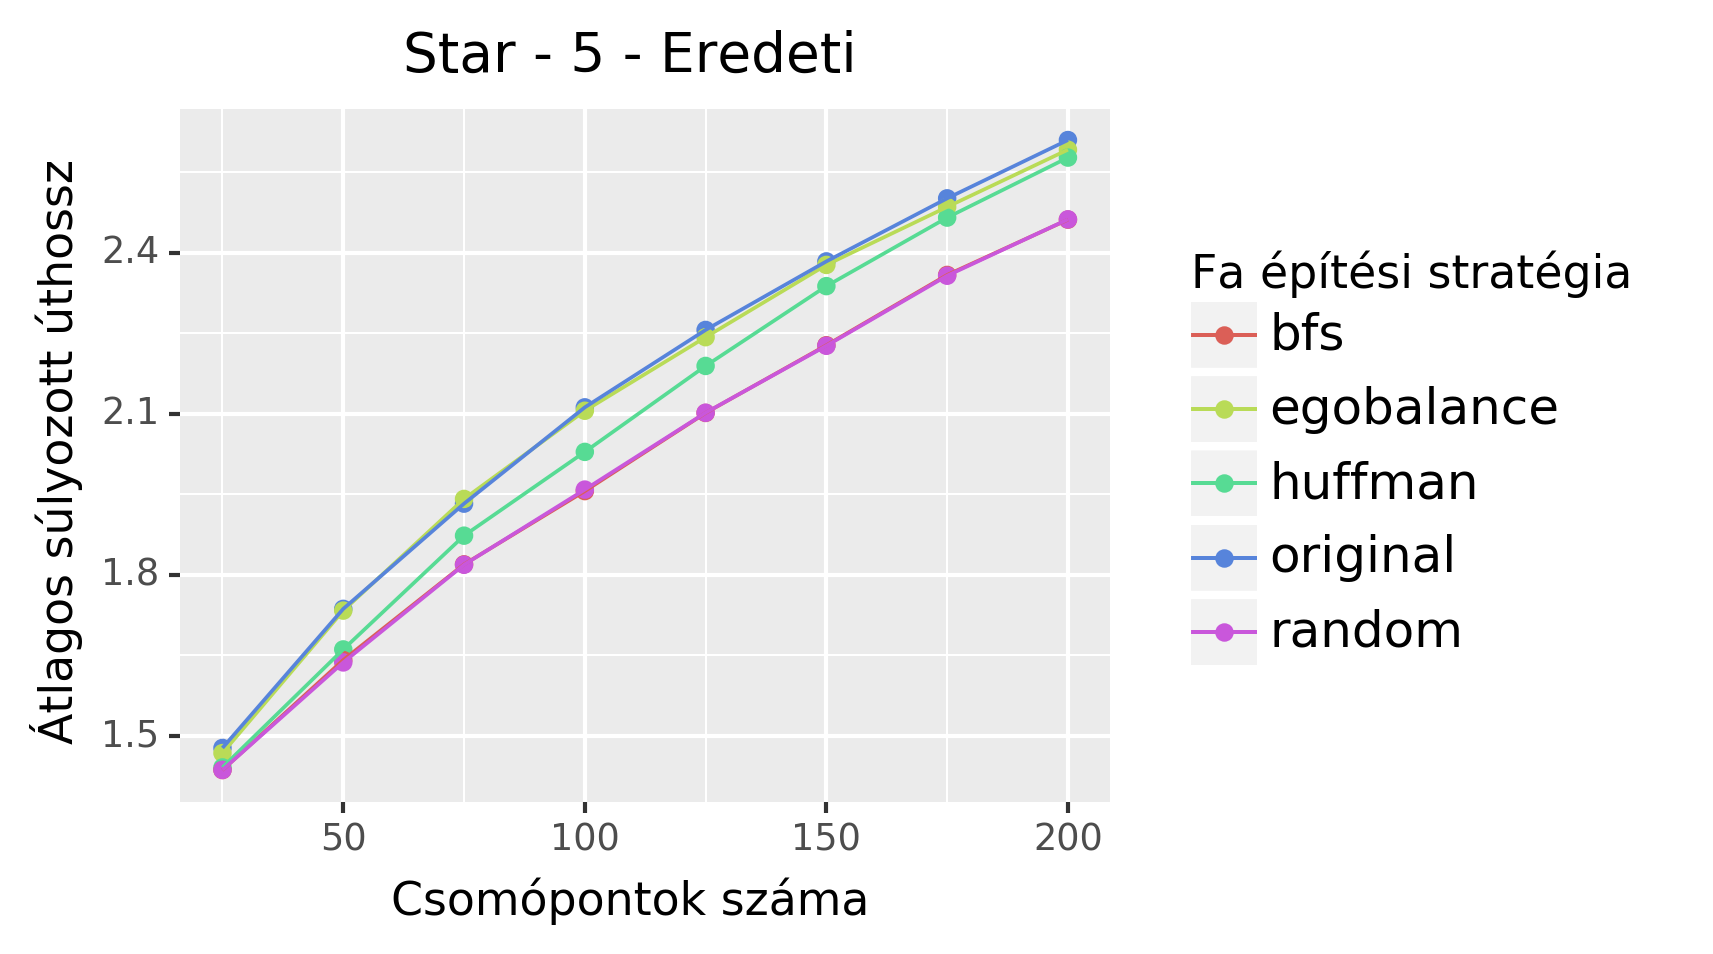
\includegraphics[width=0.9\linewidth]{pictures/star_len_e.png}
		\caption{Csillaggráf - Úthossz}
		\label{star-len}
	\end{center}
\end{figure}

Mint már láttuk a Barabási-Albert gráf esetében, itt is megvan a három egyértelmű kategória, ami teljesen megegyezik az előzővel.

\subsubsection{Módosított megépített fa mennyiség}

Az előző részben láthattuk milyen eredményeket adnak az eredeti feltétel alapján a különböző algoritmusaink.
Most nézzük meg, hogyan változik az úthossz a megépített fák számának függvényében. 
Azokat a fákat építjük meg amit ténylegesen nagyfokú, teljesül a magas fokszámú pontokra, hogy a fokszámuk legalább kétszerese az átlag fokszámnak.

Hasonlítsuk össze a Barabási-Albert gráf eredményeit a \ref{barabasi-tree-difference-len} ábrán.

\begin{figure}[H]
	\begin{center}
		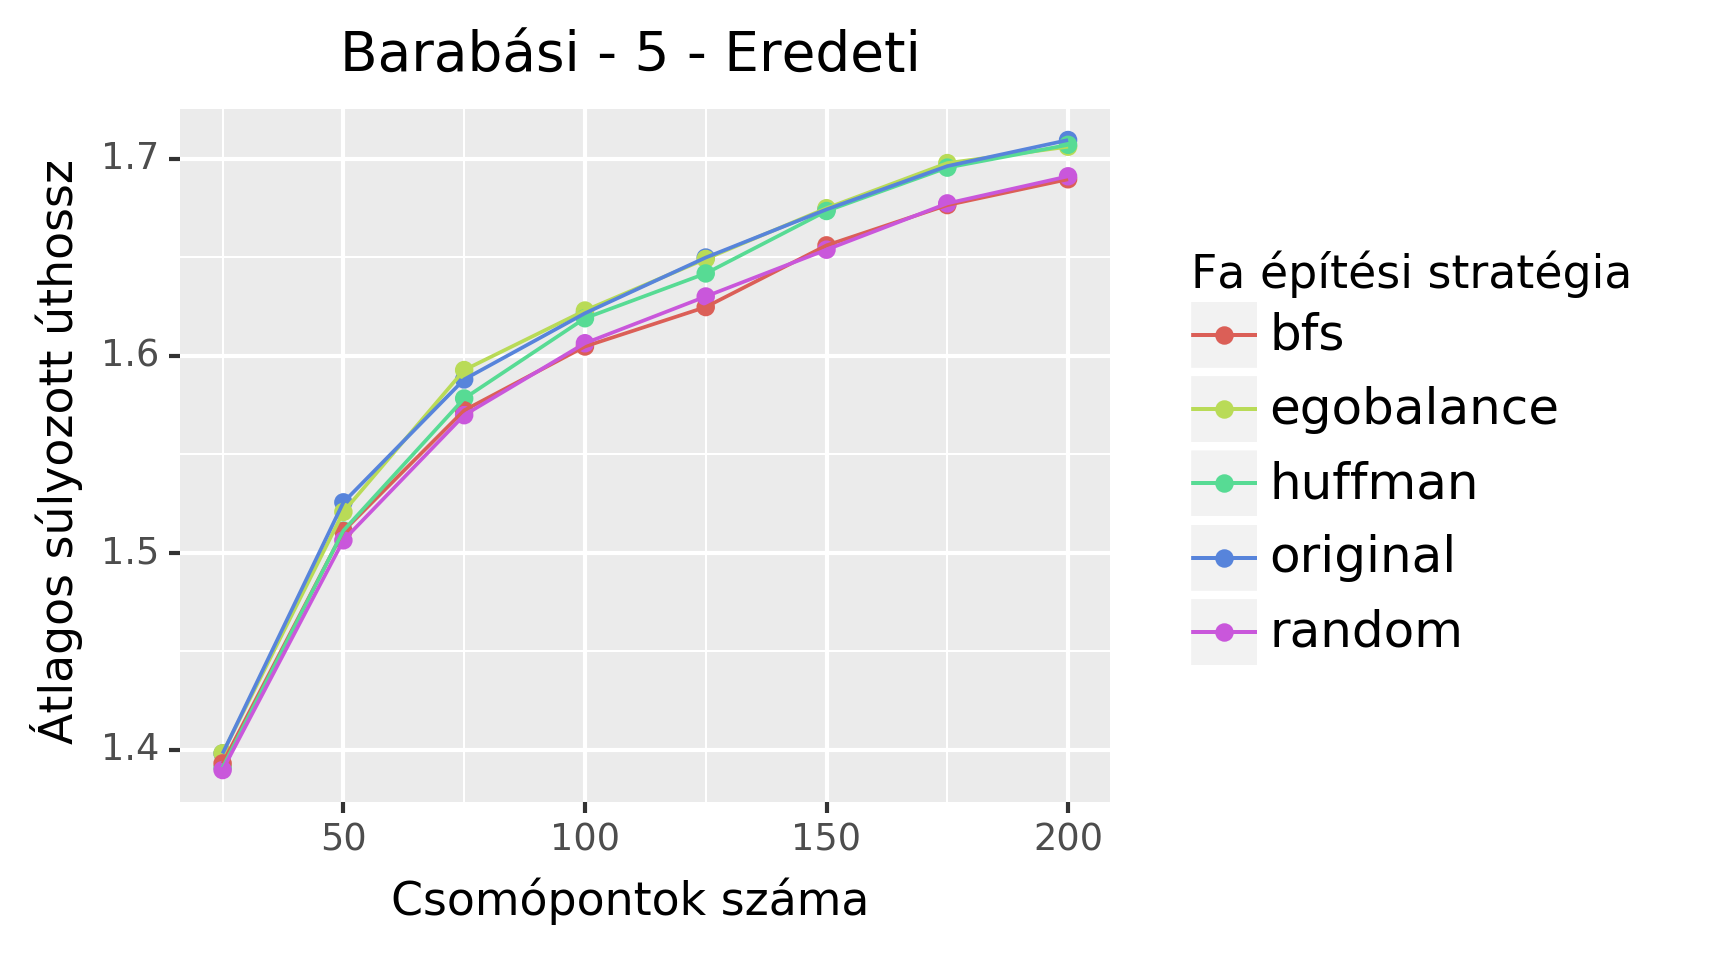
\includegraphics[width=0.49\linewidth]{pictures/barabasi_len_e.png}
		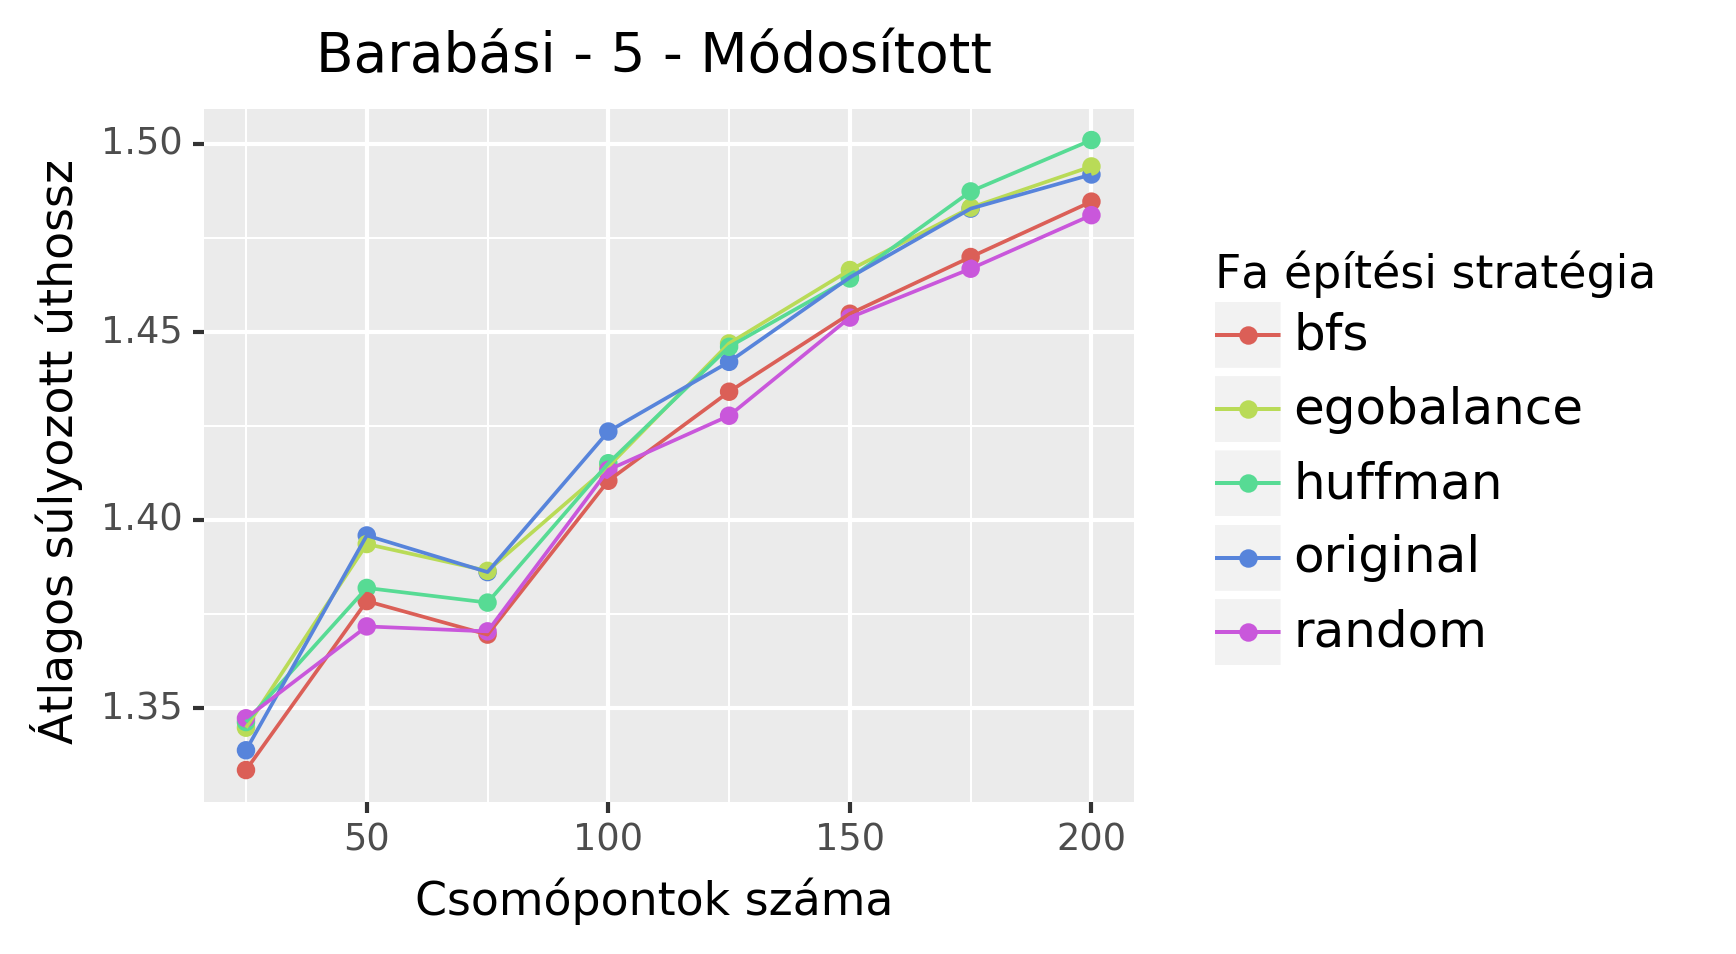
\includegraphics[width=0.49\linewidth]{pictures/barabasi_len_m.png}
		\caption{Barabási-Albert gráf - Megépített fa számosságának összehasonlítása}
		\label{barabasi-tree-difference-len}
	\end{center}
\end{figure}

Első jelentős különbség, hogy csökken az átlag úthossz.
Az gráf iránya továbbra is tartja az eredeti trendjét, egy kis beeséssel a 75 csúcsú gráfnál, de látható, hogy javít a módosítás az eredeti algoritmushoz képest.

Következő gráfunk az Erdős-Rényi gráf a \ref{erdos-tree-difference-len} ábrán.

\begin{figure}[H]
	\begin{center}
		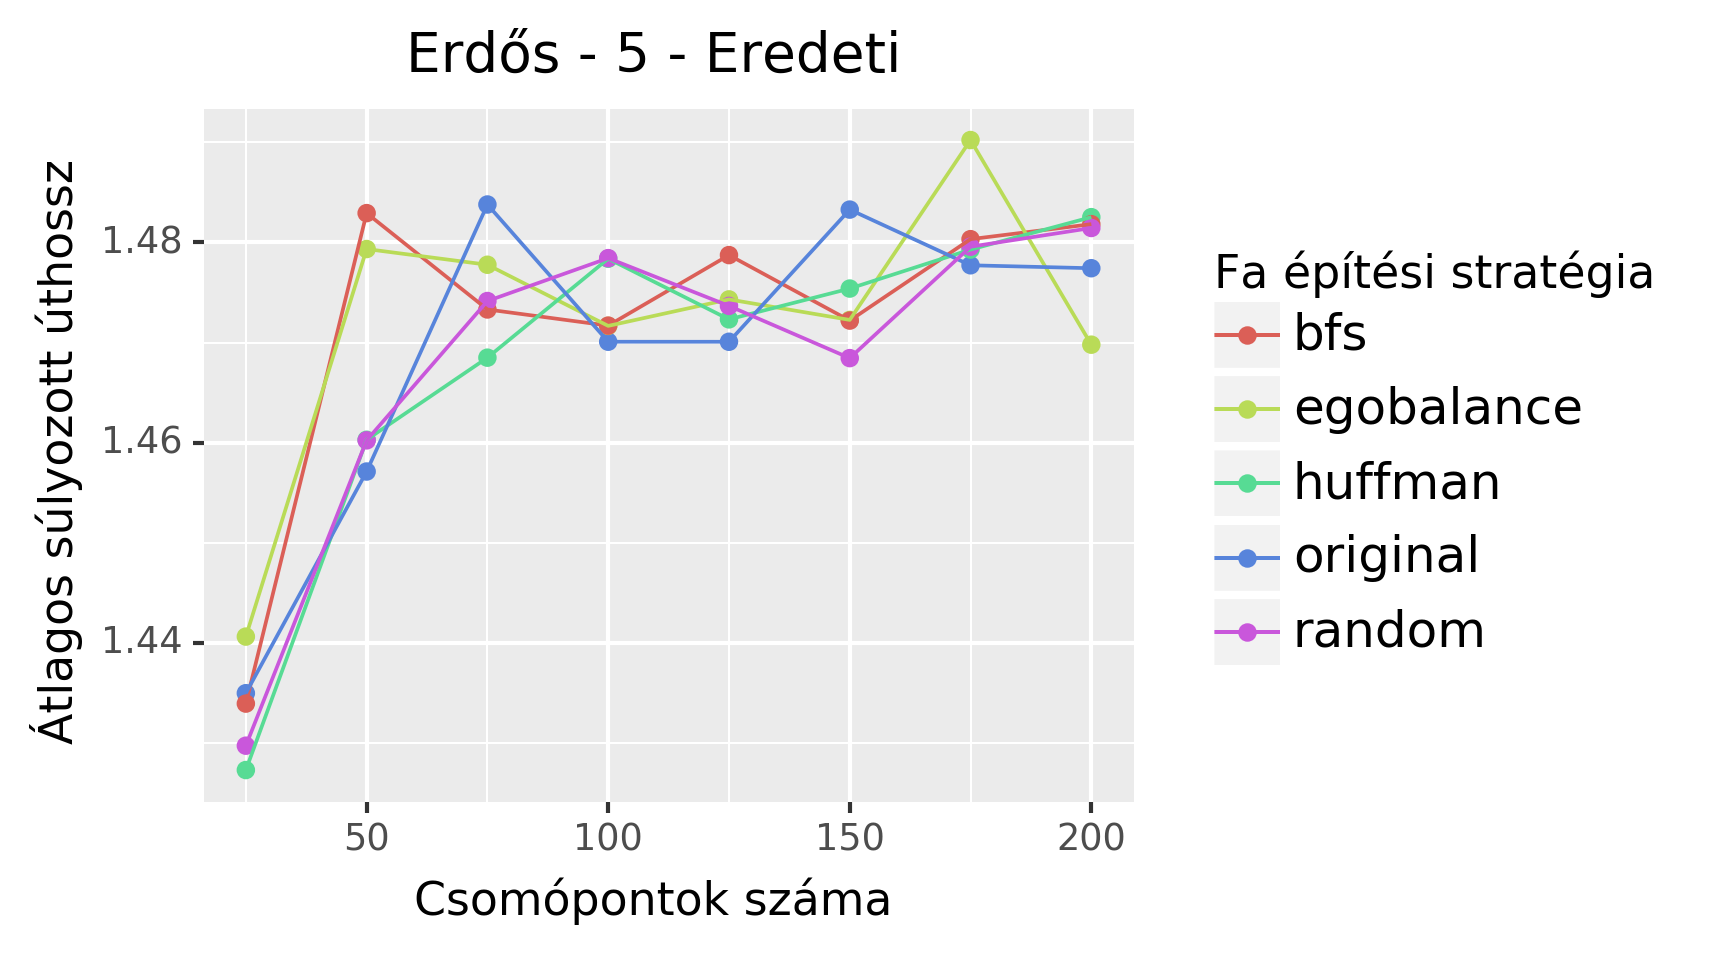
\includegraphics[width=0.49\linewidth]{pictures/erdos_len_e.png}
		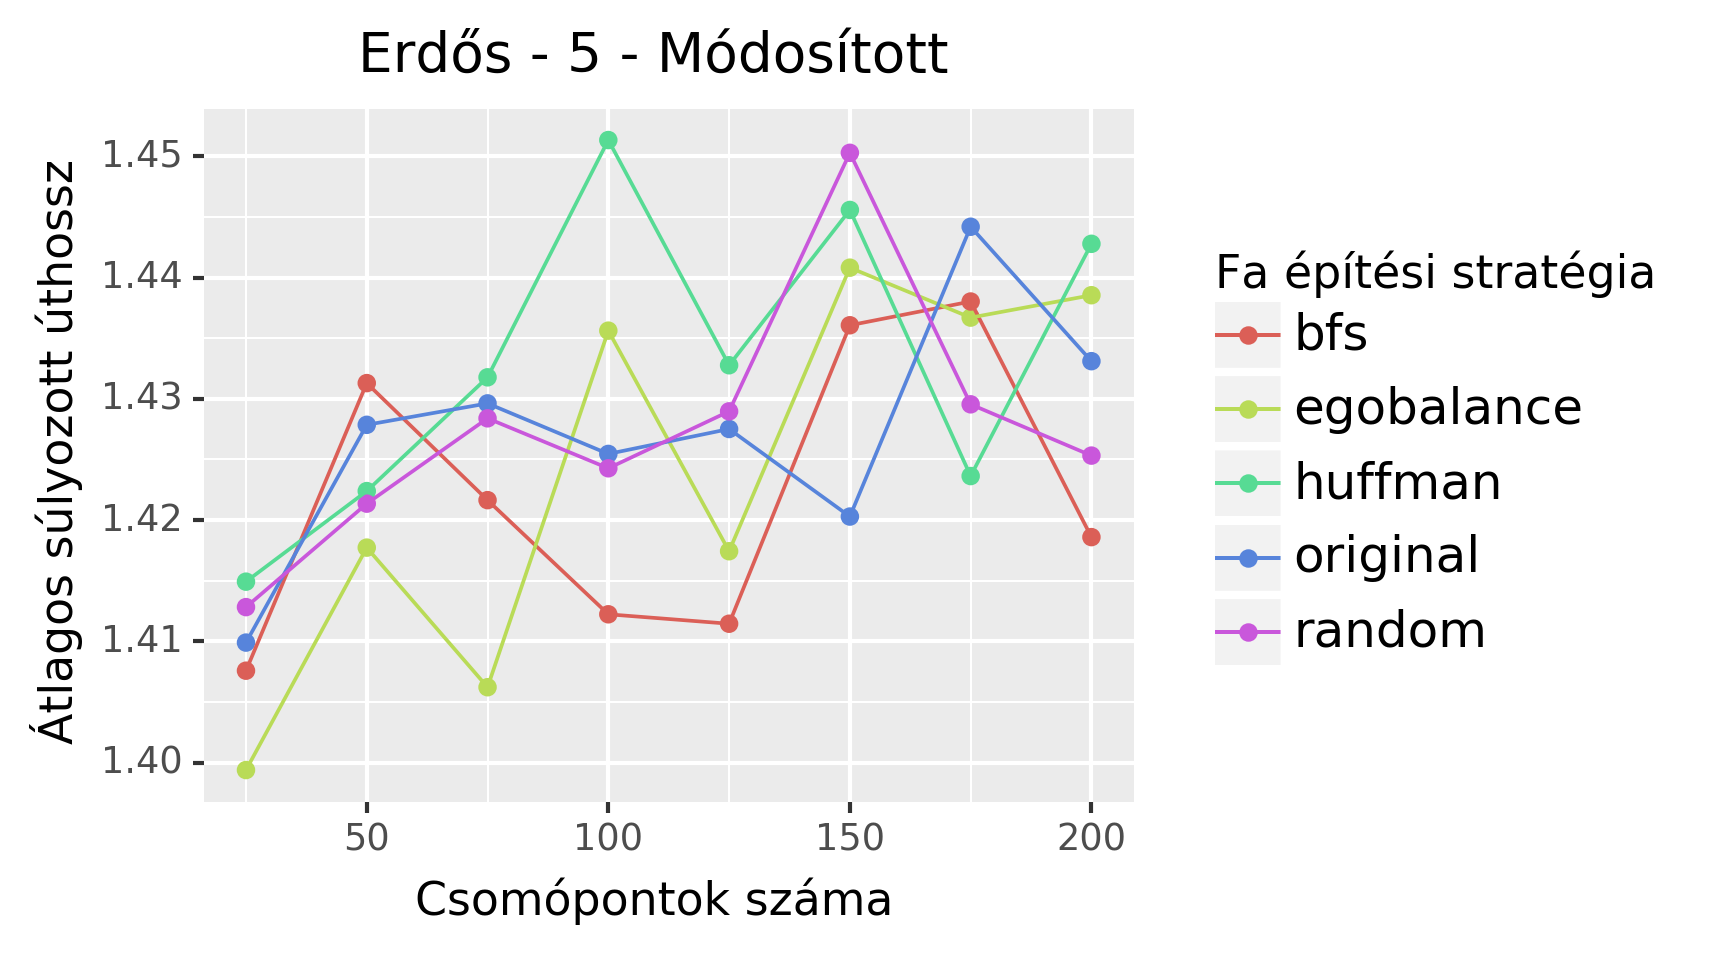
\includegraphics[width=0.49\linewidth]{pictures/erdos_len_m.png}
		\caption{Erdős-Rényi gráf - Megépített fa számosságának összehasonlítása}
		\label{erdos-tree-difference-len}
	\end{center}
\end{figure}

Amint látható, a grafikonon ismét megjelenik egy szórás, kicsit nagyobb is mint az eredetinél, de még mindig a pár százalékos határon belül. 
Az eredetihez képest az értékek kisebbek, ezzel elérve célunk a módosítás bevezetésével.

Végül nézzük meg a csillaggráfot a \ref{star-tree-difference-len} ábrán. 

\begin{figure}[H]
	\begin{center}
		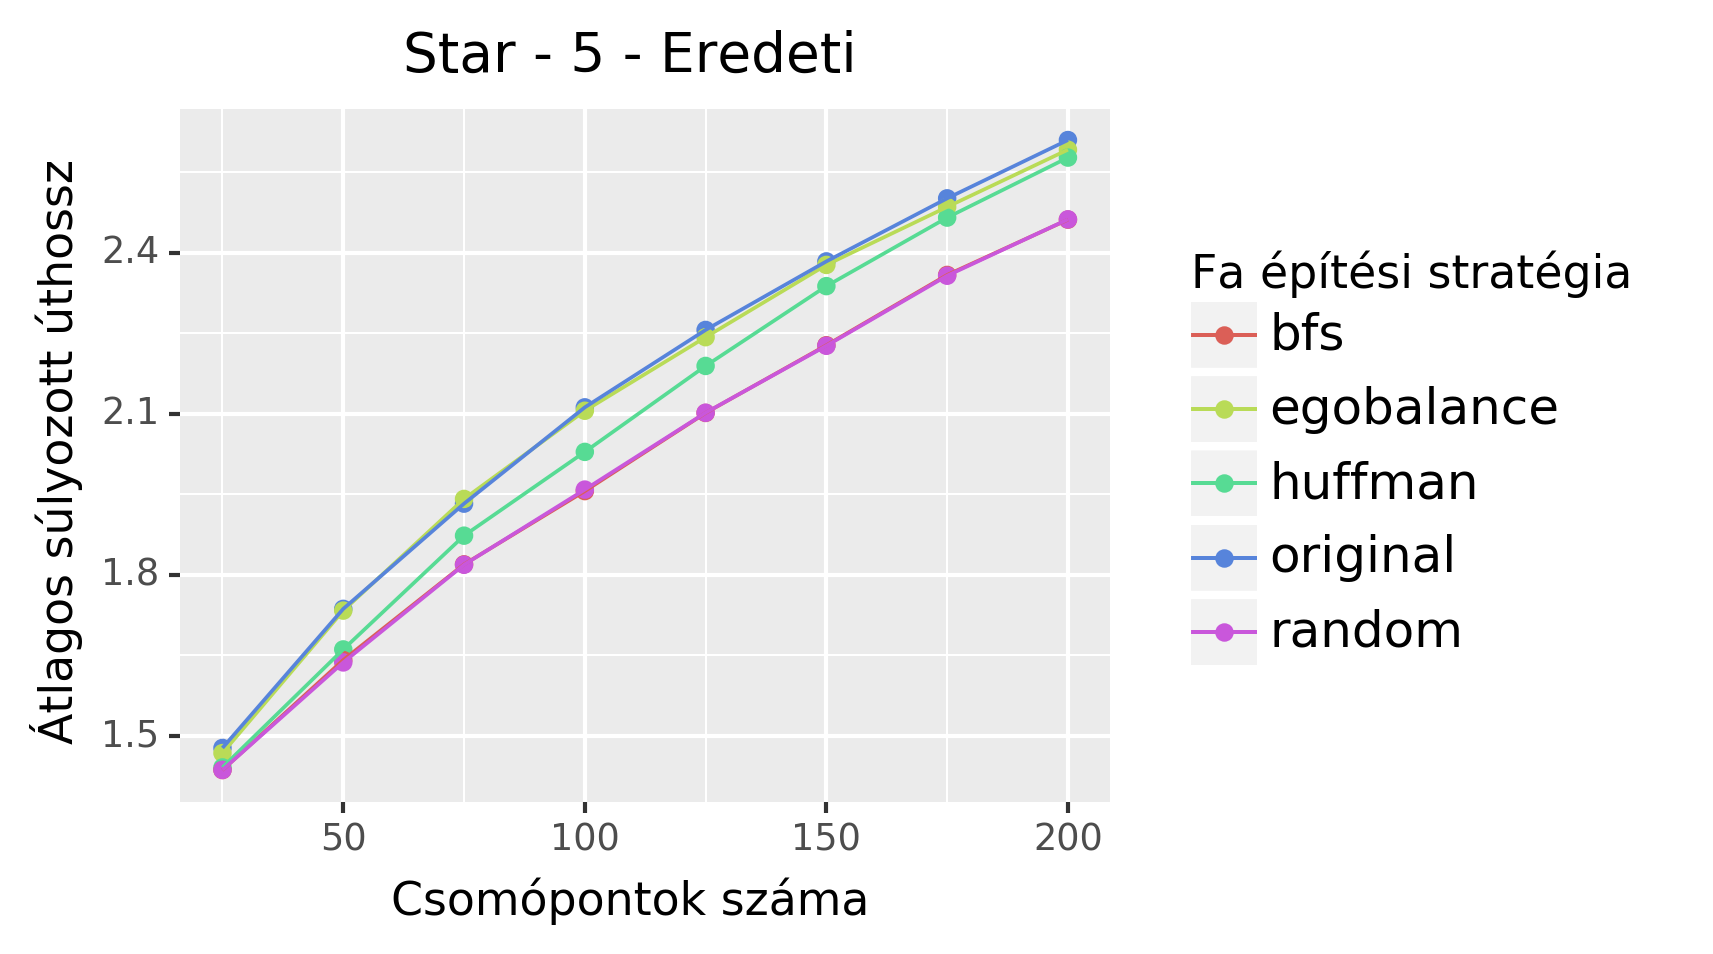
\includegraphics[width=0.49\linewidth]{pictures/star_len_e.png}
		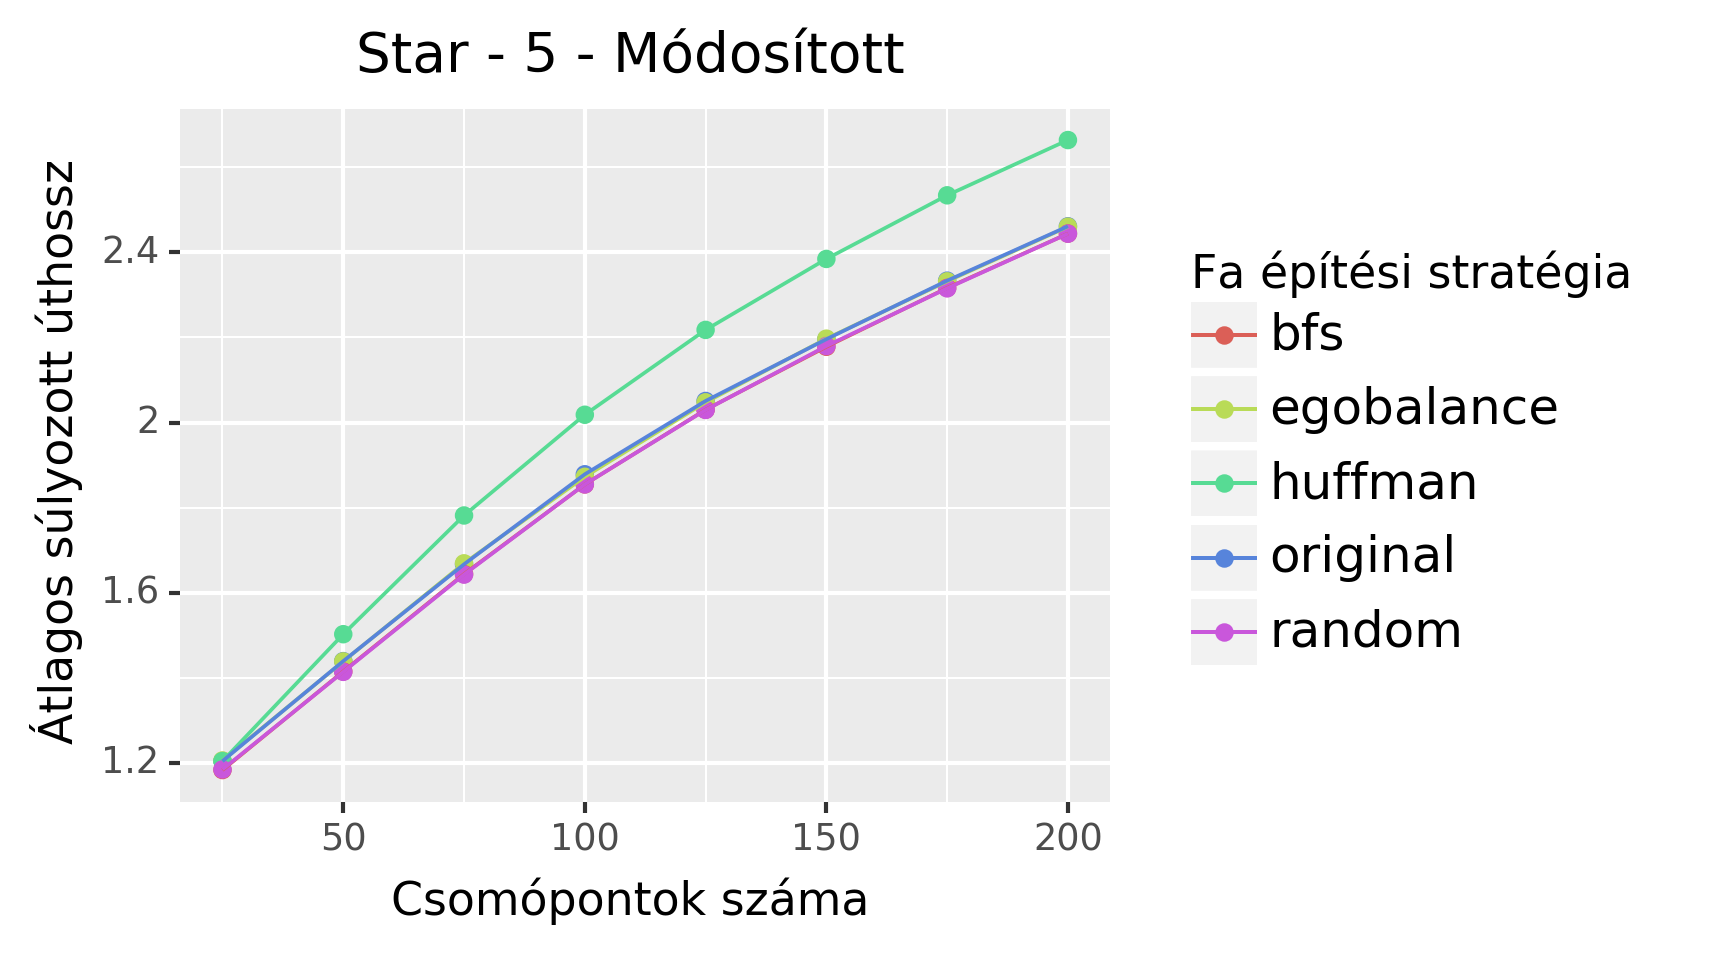
\includegraphics[width=0.49\linewidth]{pictures/star_len_m.png}
		\caption{Csillaggráf - Megépített fa számosságának összehasonlítása}
		\label{star-tree-difference-len}
	\end{center}
\end{figure}

Itt történt egy fordulat a grafikonon, először is amíg a Huffman fa alapú stratégia a közép értéket adta a két másik csoport között, itt most jelentősen rosszabb eredmény produkált.
A másik négy algoritmus meg javult az úthosszara nézve és megmaradt a relatív pozíciójuk.

\section{Torlódás}

\subsection{Általános eset}

Az úthosszhoz hasonlóan először nézzük meg, hogy az eredeti algoritmus milyen eredményt ad, attól függően mennyire sűrű a gráf.
Eredmény a \ref{density-con} ábrán.

\begin{figure}[H]
	\begin{center}
		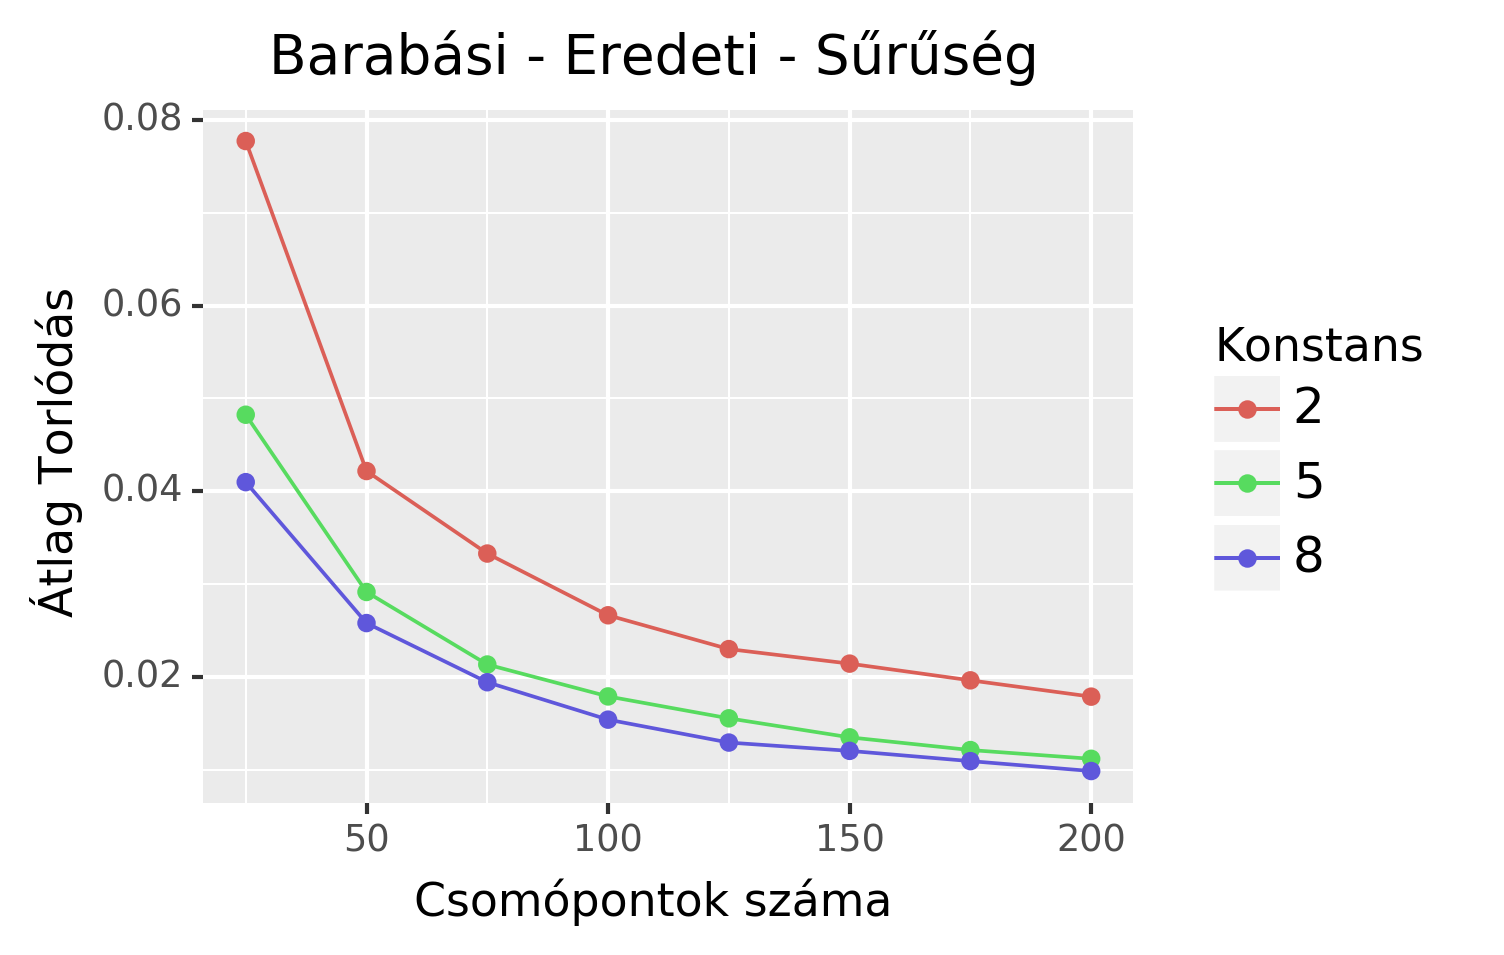
\includegraphics[width=0.9\linewidth]{pictures/density_con.png}
		\caption{Torlódás és demand mátrix kitöltöttségének kapcsolata }
		\label{density-con}
	\end{center}
\end{figure}

A grafikonon a Barabási-Albert gráf eredményei látható, az eredeti számú megépített fa mennyiséggel és a fák pedig az eredeti algoritmussal készültek el.
A hálózatban szereplő összes él súlya 1.
Mint látható a grafikonon, minél ritkább a mátrix, annál nagyobb a torlódás. 
Egy fontos észrevétel a két metrika között, még az úthossz átlagosan az egész mátrixra nézve adta meg az eredményt, addig a torlódás az egyértelműen a legnagyobb torlódás az útválasztási sémán.
Ezért ha kevés éllel rendelkezik a gráf, annál kevesebb lehetősége van olyan élt választani az algoritmusnak, ahol még alacsony a torlódás.
A további grafikonoknál már csak a konstans 5 értékű eredményeket fogom vizsgálni, mivel az ad egy jó közelítést az átlagos torlódása.

\subsection{A fa építő algoritmusok összehasonlítása}

\subsubsection{Eredeti megépített fa mennyiség}

Az általános eset után, most vizsgáljuk meg, hogy a különböző fa építési stratégiák, hogy befolyásolják a torlódást.

Első véletlen gráf ismét a Barabási-Albert gráf, ahol az eredeti mennyiségű fát építjük meg. 
Eredmény a \ref{barabasi-con} ábrán.

\begin{figure}[H]
	\begin{center}
		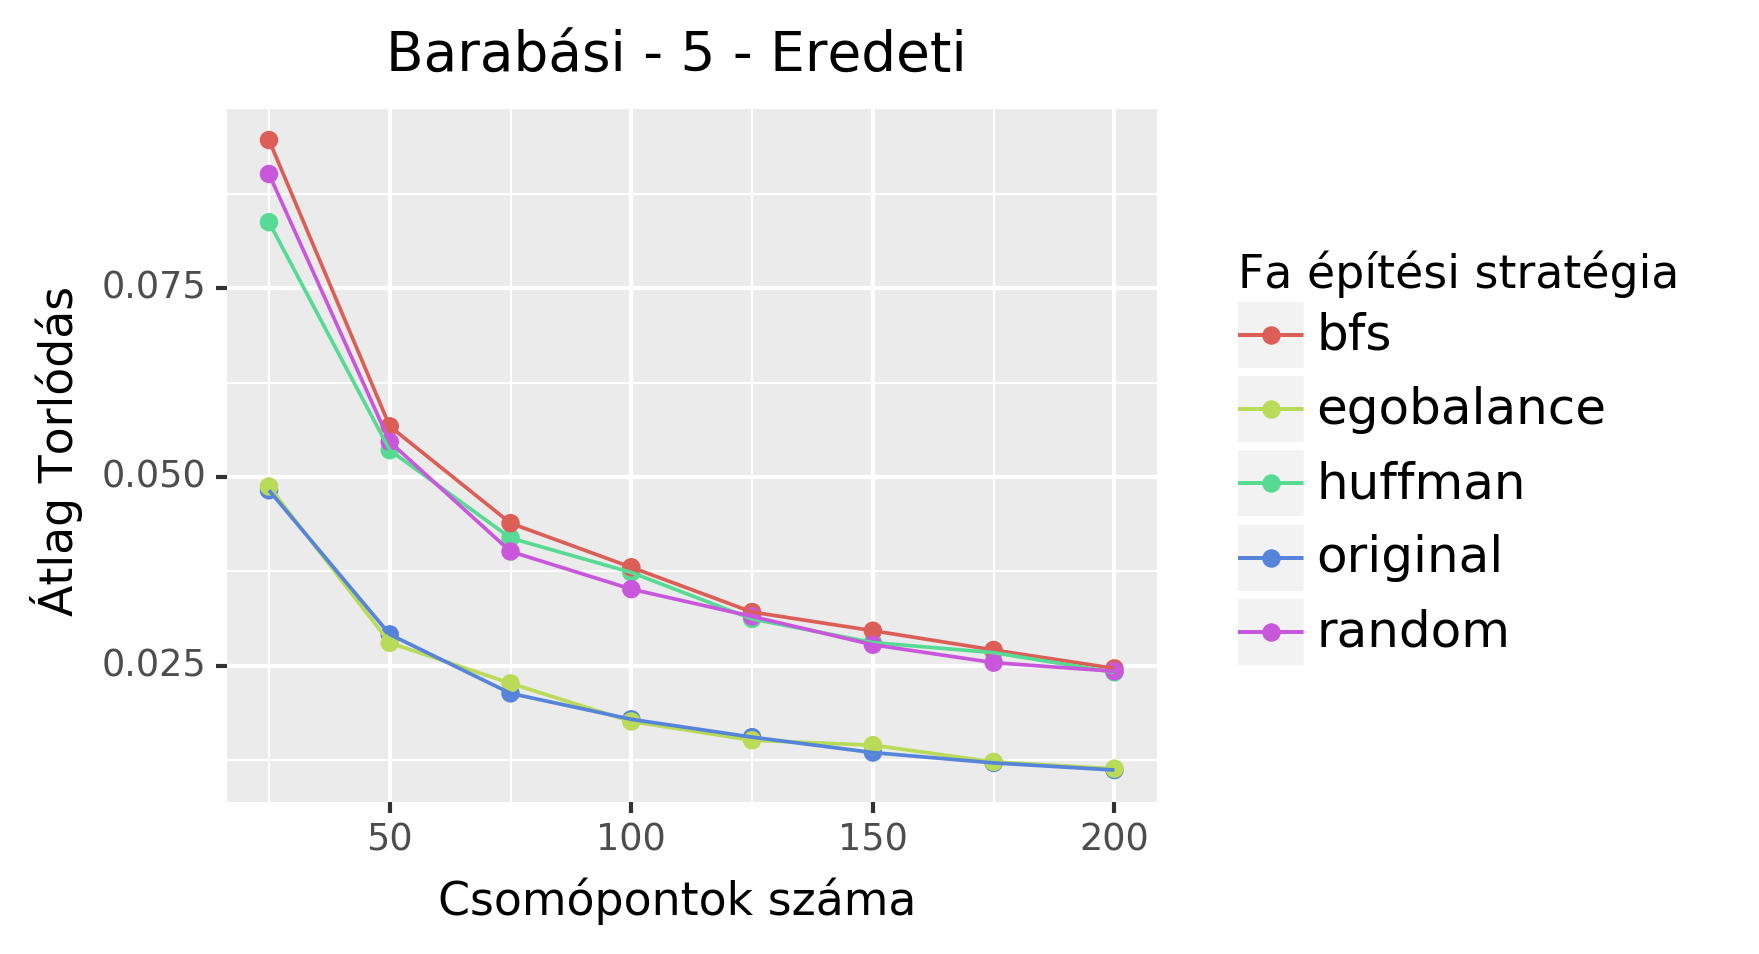
\includegraphics[width=0.9\linewidth]{pictures/barabasi_con_e.png}
		\caption{Barabási-Albert gráf - Torlódás}
		\label{barabasi-con}
	\end{center}
\end{figure}

A grafikonon látható, hogy két csoportba lehet besorolni az algoritmusokat. 
Az elsőbe tartozik az EgoBalance és az Eredeti algoritmus.
Ezek adják a legjobb eredményt és szinte azonosak.
A másik csoportba tartozik a maradék három algoritmus, a Sorfolytonos-, a Random- és a Huffman fa.
Itt egyértelmű miért jött ki ez az eredmény, mivel ez a három algoritmus egyáltalán nem veszi figyelembe a tényezőt, hogy mekkora a torlódás.

Következő véletlen gráf típus az Erdős-Rényi gráf, itt is az eredeti számú fát építjük meg. 
Eredmény a \ref{erdos-con} ábrán.

\begin{figure}[H]
	\begin{center}
		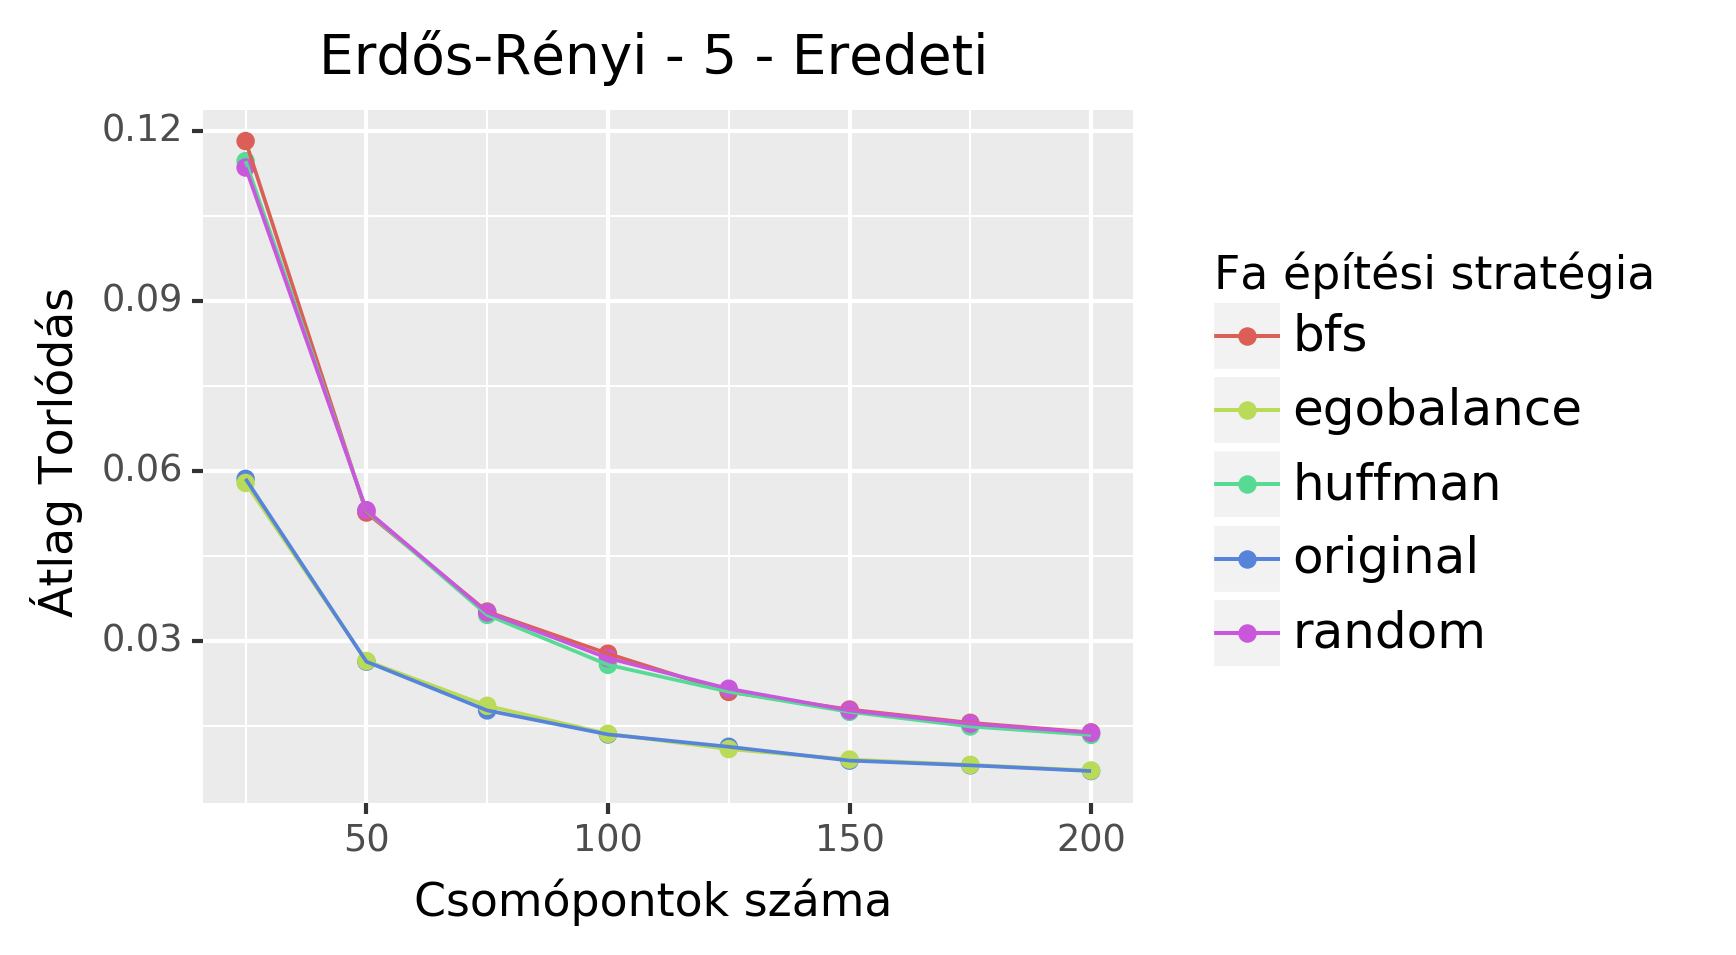
\includegraphics[width=0.9\linewidth]{pictures/erdos_con_e.png}
		\caption{Erdős-Rényi gráf - Torlódás}
		\label{erdos-con}
	\end{center}
\end{figure}

A grafikon szinte megegyezően ugyanazt az eredmény mutatja mint a Barabási-Albert gráf esetén.
Két csoport, ahol még mindig az Eredeti és az EgoBalance teljesítenek a legjobban.

Végül pedig nézzük meg a csillaggráfot az eredeti fa mennyiséggel a \ref{star-con} ábrán.

\begin{figure}[H]
	\begin{center}
		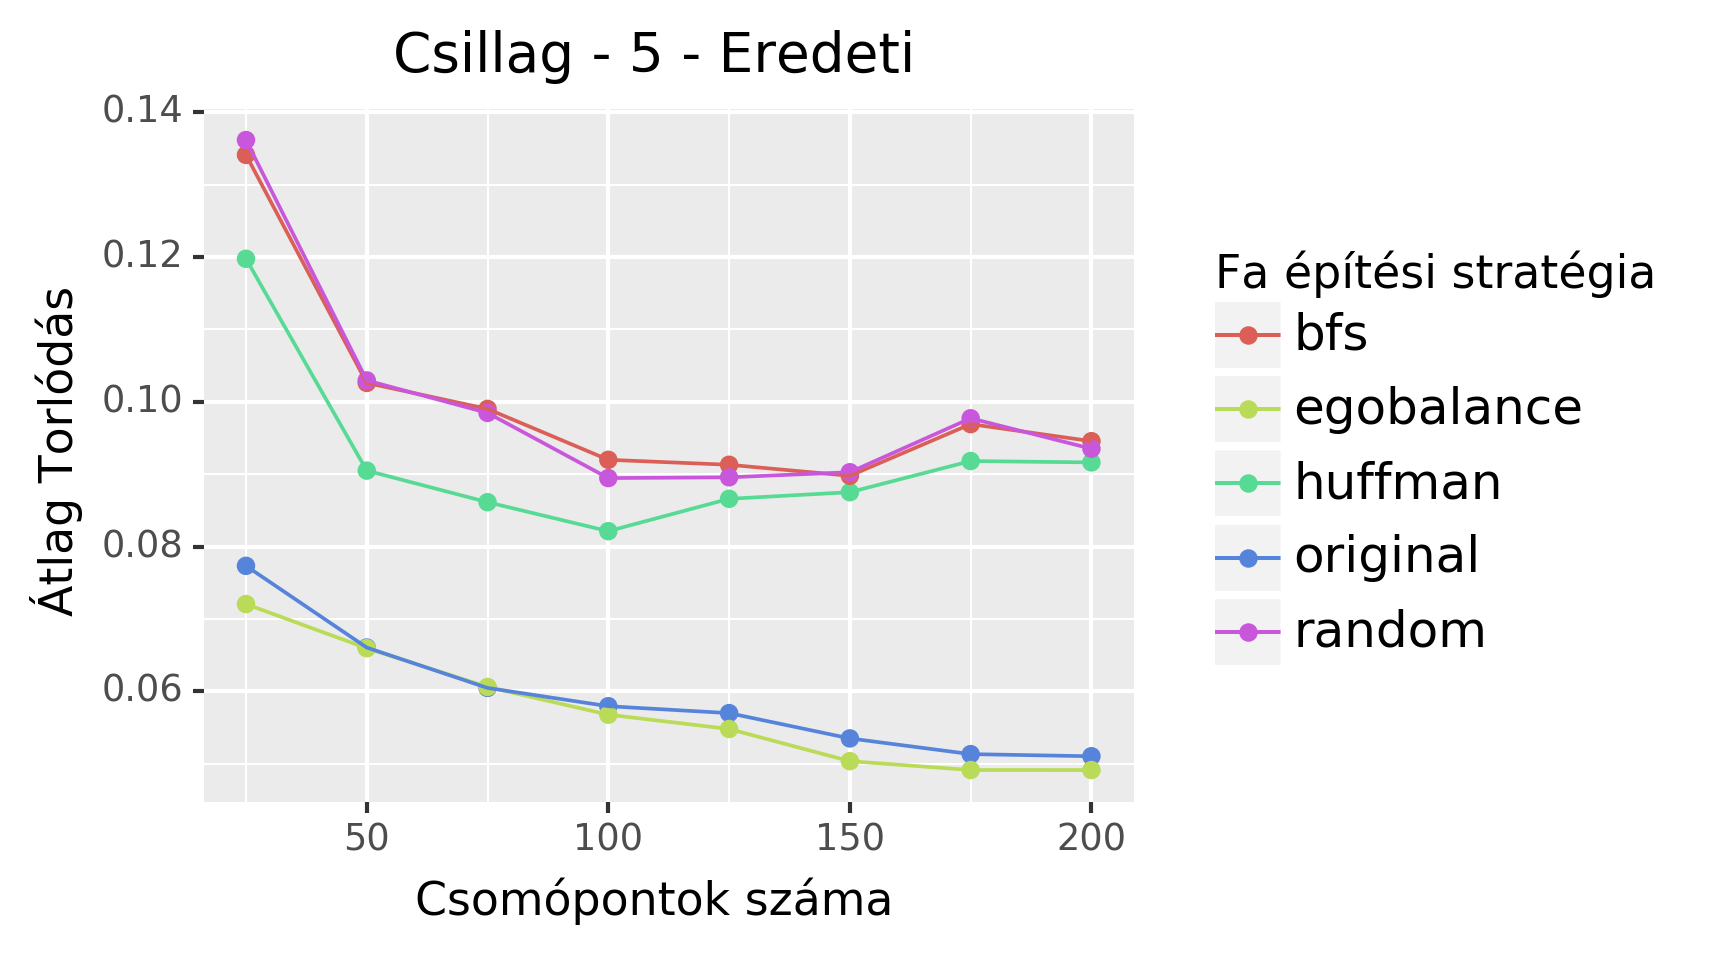
\includegraphics[width=0.9\linewidth]{pictures/star_con_e.png}
		\caption{Csillaggráf - Torlódás}
		\label{star-con}
	\end{center}
\end{figure}

Itt már elhatárolódik a Huffman fa a Sorfolytonos és Random fáktól, de nem eléggé, hogy megközelítse az Eredetit vagy az EgoBalance-ot.

\subsubsection{Módosított megépített fa mennyiség}

Az előző részben láthattuk milyen eredményeket adnak az eredeti feltétel alapján a különböző algoritmusaink.
Most nézzük meg, ha változik a torlódás a megépített fák mennyiségének függvényében. 
Azokat a fákat építjük meg amit ténylegesen nagyfokúak.

Hasonlítsuk össze a Barabási-Albert gráf eredményeit a \ref{barabasi-tree-difference-con} ábrán.

\begin{figure}[H]
	\begin{center}
		\includegraphics[width=0.49\linewidth]{pictures/barabasi_con_e.png}
		\includegraphics[width=0.49\linewidth]{pictures/barabasi_con_m.png}
		\caption{Barabási-Albert gráf - Fa számosság összehasonlítás}
		\label{barabasi-tree-difference-con}
	\end{center}
\end{figure}

Számottevően jelentős különbség nem jelentkezik a két eset között.

Következő gráfunk az Erdős-Rényi gráf a \ref{erdos-tree-difference-con} ábrán.

\begin{figure}[H]
	\begin{center}
		\includegraphics[width=0.49\linewidth]{pictures/erdos_con_e.png}
		\includegraphics[width=0.49\linewidth]{pictures/erdos_con_m.png}
		\caption{Erdős-Rényi gráf - Fa számosság összehasonlítás}
		\label{erdos-tree-difference-con}
	\end{center}
\end{figure}

Jelentős különbség itt sem figyelhető meg.

Végül nézzük meg a csillaggráfot a \ref{star-tree-difference-con} ábrán. 

\begin{figure}[H]
	\begin{center}
		\includegraphics[width=0.49\linewidth]{pictures/star_con_e.png}
		\includegraphics[width=0.49\linewidth]{pictures/star_con_m.png}
		\caption{Csillaggráf - Fa számosság összehasonlítás}
		\label{star-tree-difference-con}
	\end{center}
\end{figure}

Itt már jelentkezik különbség, az elején még hasonló a két gráf, de ahogy növeljük a csomópontok számát, a módosított algoritmus rosszabb eredményt eredményez, mint az eredeti algoritmus.
Ennek az az oka, hogy a megépült fák sekélyek, de ahogy növekedik a élek száma, egyre nagyobbak lesznek ezek a fák.
Szóval a torlódás összpontosul egy helyre, erre pedig példa a \ref{inbalance} ábra.

\begin{figure}[H]
	\begin{center}
		\includegraphics[width=0.7\linewidth]{pictures/Figure_5.png}
		\caption{Csillaggráf - Egófa az eredeti algoritmus alapján}
		\label{inbalance}
	\end{center}
\end{figure}

A hálózat ami ezt az Egófát eredményezte az 30 csomópontból áll, 5 csillagot tartalmaz és maximális $\Delta$ fokszám pedig 12. 
Mint látható egységesen helyezkednek el a csomópontok és a legtávolabbi levél is csak kettő mélységre helyezkedik el.
Abban az esetben, mikor a csomópontokból relatív kevés van, és alacsony fák kapcsolódnak össze, a torlódás is várhatóan alacsony lesz. 
Ahogy nő a csomópontok száma és eléri a többszörösét a maximális fokszámnak, nehéz utak alakulnak ki és így növekszik a torlódás is.

\chapter{Összefoglalás}

\section{Diplomamunka eredménye}

A diplomamunka keretén belül feldolgozásra került a Demand-Aware Network Design with Minimal Congestion and Route Lengths \cite{avin_demand-aware_nodate} cikk.
A szerzők arra kerestek megoldást, hogy lehetne csökkenteni a torlást és az úthosszt az adatközpontokban.
A felvázolt megoldásuk mellett adtak egy felső korlátot, amivel az algoritmus ad egy közel optimális megoldást.

\subsection{Keretrendszer}

A diplomatikusában megvalósít keretrendszer segítségével a szerzők megoldása gyakorlati tesztelés alá lett vetve.
Itt több fajta véletlen gráffal lett szimulálva a lehetséges hálózatok és az azokon folyó adatforgalom.
Az Erdős-Rényi modell segítségével modelleztük azt az esetet, mikor a kommunikáció egyenletesen eloszlik a hálózaton és nem centralizálódik több nagyobb szerver köré a forgalom.
A Barabási-Albert modell segítségével már nagyobb klasztereket kaptunk, mivel akik később csatlakoztak, azok mindig választottak még $m$ régi csomópontot.
Így a legelsők a hálózatban nagyobb eséllyel kaptak több kapcsolatot.
Végül pedig az extrém eset, a csillaggráf, mikor több nagyobb csomópont köré összpontosul a forgalom.

Az így megkonstruált gráfokon az eredmények azt mutatják, hogy a cikkben meghatározott "optimális" eset egy határozottan magasabb felső korlát, mint amire valójában szükség van.
A megadott $\Delta = 12\rho$ fokszám egy túl nagy felső korlát, mivel olyan gyorsan nő ez a szám, hogy már $\Delta = 4\rho$ esetben is, az algoritmus lefuttatása után bőven meghaladja a valóban szükséges fokszámot.
Ez azt eredményezi, hogy az összes kapcsolat egy köztes segítő csomópont segítségével majdnem direkt kapcsolódik.
Ezért nem tudnak elég magas fák kialakulni, hogy a különböző algoritmusok érdemi különbséget nyújtsanak.
Így tesztelés során, egy jól meghatározott korlát segítségével voltak a tesztek lefuttatva. 
Az korlát alapját a piacon jelenleg forgalomban lévő Ethernet switch portok száma adta, ami $\Delta \in [10, 16, 24, 48]$ lett.

\subsection{Algoritmusok}

Az cikkben megfogalmazott cl-Dan algoritmus hagy némi helyet az implementálónak a részletek terén, mivel nem teljesen írja le egy helyzetben a helyes lépést.
Ez alapján született kettő algoritmus, az Eredeti és az EgoBalance, ami a csere lépésben felmerülő szülő nélkül maradt gyerekek újra csatlakoztatását hivatott megoldani.
Itt az Eredeti helyben mozgatta át a nehezebb gyereket a szülő pozíciójára, addig az EgoBalance egy természetesebb, az alapul szolgáló adatstruktúrára bízta az újra eloszlást.
Eredmény szempontjából a kettő algoritmus nagyon hasonló, és lényegbeli különbség a mérési hiba korlátain belül szerepel.

Annak érdekében, hogy a valós hozzávetési alapunk legyen a módszer teljesítményéhez további másik fa építési módszerek is meg lettek vizsgálva.
Ezek alapjául a Huffman fa szolgált és ezekből lett három különböző algoritmus, amik rendre a Huffman-, Sorfolyotonos- és Véletlen fák voltak.

A Huffman kódolásban is használt fa lett az első algoritmus, ami az úthosszt hivatott javítani.
Ennek eredménye helyenként tényleg jobb lett, mint az Eredeti esetben, de mivel nem csak ez az egy szempontból kell jól teljesíteni, így figyelembe kell venni a torlódást is.
Ebből a szempontból már határozottan nem teljesített jól, mert a Huffman fa ágai között akár másfélszeres szorzó különbség előfordulhat, így leterhelt utak jönnek létre. 

Következő algoritmus ami létrejött az a Sorfolytonos fa.
Itt egyelten szempont volt figyelembe véve, építsünk egy teljes fát.
Ezzel a módszerrel mindig a legkisebb fák jöttek létre és így ez eredményezte mindig a legrövidebb utakat.
Torlódás szempontjából ugyanolyan rosszul teljesített mint a Huffman fa, mivel itt sem volt figyelme véve ez a szempont.
Mivel ez volt a legjobb úthosszra adott algoritmus, lehet érdemes lenne további kutatás folytatni annak érdekében, hogy hogyan lehet a torlódást javítani egy ilyen hálózatban.

Végül a Random fa, ami nem különbözik különösebben a Sorfolyotnostól.
Ennek az eredménye sem lett jobb, mint amire épül, ám lehetőség van arra, ha épp úgy helyezkednek el az elemek, hogy az torlódás szempontjából is kedvező, akkor van némi esély arra, jobb eredményt ad.

Ezekből az eredményekből az látszik, hogy a cikkben szereplő algoritmus megfelelő a céljára, ám ez nem zárja ki annak a lehetőséget, hogy egy másfajta javításibeli megközelítést is kivizsgáljuk. 

\pagebreak

\subsection{Kritikus pontok megfontolása}

A második javítási mód előtérbe helyezi azt a szempontot, hogy mérlegeljük a hálózatban szereplő ténylegesen leterhelt pontokat.
Ezzel célzottabban tudjuk a hálózat kritikus pontjait orvosolni és elejét vehetjük az olyan esteknek, hol nincs szükség átépítésre.
Ezzel csökkenthetjük a számítás igényét az algoritmusnak és egyúttal még rövidebb utakat is érünk el a legtöbb esetben.
Mivel ez a megközelítés csak finomítja a cl-Dan első lépését, ami alapján osztályozzuk a pontokat, így legrosszabb esetben is visszaértünk a kiindulási algoritmushoz és soha nem lesz rosszabb attól.
A mérések azt mutatják, hogy az úthossz határozottan csökken, de a torlódásra az esetek túlnyomó részében nincs kihatással, ám vannak elfajult esetek, ahol rosszabbat eredményez.

\section{Konklúzió}

A cikkben \cite{avin_demand-aware_nodate} meghatározott algoritmus a mérések alapján megfelel a céljára.
Az Eredeti és EgoBalance megközelítések között különbség minimális így, az olvasónak lehetősége van kicsit kísérletezni, milyen megközelítést szeretne használni.
A hasonló célra létrehozott algoritmusok közül pedig a Sorfolyonos ami érdekes információval szolgált, ezért érdemes lenne még ez irányban kutatást végezni.


\chapter{Köszönetnyilvánítás}

Szeretnék köszönetet nyilvánítani témavezetőmnek Lukovszki Tamás, PhD egyetemi docensnek, amiért felajánlotta és vezetett a téma kidolgozásában és megvalósításában.
Továbbá még szeretném megköszönni Veress Orsolya támogatását is, a munka korrektúrájában nyújtott segítségért.  


\bibliographystyle{abbrv}
\bibliography{refrences}

	
\end{document}